%\chapter{Mode Splitting and Coupling}
\chapter{模式分裂与耦合}
\label{chapter:splitting_and_coupling}

\enlargethispage{-0.5\baselineskip}

\iffalse
The splitting of the free oscillations of the Earth was first
observed following the great 1960 earthquake in Chile;
\index{Chile 1960 earthquake}%
the apparent doublet character of the ${}_0{\rm S}_2$
and ${}_0{\rm S}_3$ multiplets was immediately attributed
to the rotation of the Earth, as we recounted in the historical
introduction.  Rotation and the associated hydrostatic
ellipticity of figure contribute significantly to the splitting
and coupling of the gravest free oscillations; however, splitting
due to other perturbations is often much more significant.  Observations
of this non-hydrostatic splitting may be used to constrain the
elastic lateral heterogeneity and anisotropy---and thus the
internal dynamics---of the Earth.  This chapter begins with
a brief introduction to hydrostatic figure theory, and then
considers the seismologically observable effects of rotation,
hydrostatic ellipticity, large-scale mantle heterogeneity,
and transverse isotropy of the inner core.
We base our analysis of these effects upon the
general formulation of degenerate and quasi-degenerate
perturbation theory presented in Chapter 13, introducing
a number of minor modifications and approximations
for convenience.  First, we take the unperturbed
spherical Earth model to be the {\em anelastic
terrestrial monopole\/}; spherically symmetric
\index{terrestrial monopole}%
attenuation is incorporated into the monopole by
modifying the degenerate reference eigenfrequencies:
$\om_k\rightarrow\om_k+i\gamma_k$, where $\gamma_k$
is the degenerate decay rate.  The elastic and anelastic
structural perturbations are thus considered to be
{\em purely aspherical\/}.
Second, the first-order renormalization terms introduced
in the general analysis are small; in this chapter we drop
them upon occasion for simplicity.  Third, the contribution
of aspherical anelasticity to the renormalization is particularly
small; it will be ignored completely.
\fi
%%%
地球自由振荡的分裂是在~1960~年智利大地震之后被首次观测到;正如在历史介绍所述,多重态~${}_0{\rm S}_2$~和~${}_0{\rm S}_3$~的明显的双峰特征被立即归因于地球的自转效应。自转和相应的形状流体静力学椭率对最强自由振荡模式的分裂与耦合有着重要作用;然而,由其他微扰产生的模式分裂往往更为重要。对这种非静力学分裂的观测可用来约束地球的弹性横向不均匀性和各向异性,从而进一步约束地球内部动力学。本章首先简要介绍流体静力学形状理论,然后考虑自转、流体静力学椭率、大尺度地幔不均匀性及内核横向各向异性的地震学可观测影响。我们将基于第~13~章的简并和准简并微扰理论中的一般性公式来分析这些影响,为方便起见,引入了一些小的修正和近似。首先,我们将未扰动球形地球模型视为非弹性地球单极;通过修改简并参考本征频率~$\om_k\rightarrow\om_k+i\gamma_k$(其中~$\gamma_k$~为简并衰减率),将球对称衰减纳入单极中。由此,弹性和非弹性结构微扰可被考虑成纯非球形的。其次,在一般形分析中引入的一阶重归一化项很小;在本章中,为简单起见,我们偶尔忽略它们。最后,非球形非弹性对重归一化的贡献极小,将被完全忽略。
%%%

%\section{Hydrostatic Ellipticity}
\section{流体静力学椭率}
\index{hydrostatic ellipticity|(}%
\index{ellipticity|(}%
\label{section:shape of the earth}

\iffalse
The shape of a slowly rotating planet in hydrostatic equilibrium
is described by the classical theory of Clairaut (\citeyear{clairaut43}).
Modern accounts of this venerable topic may be found in Jeffreys
(\citeyear{jeffreys70}) and Bullen (\citeyear{bullen75}).
We give our own brief summary of hydrostatic equilibrium
theory here, following the treatment by Chandrasekhar \& Roberts
(\citeyear{chandrasekhar&roberts63}).  All of our considerations
are valid to first order in the centrifugal-to-gravitational-force
ratio $\Omega^2a^3\hspace{-0.5 mm}/GM$,
where $\Omega$ is the sidereal rate
of rotation, $a$ and $M$ are the mean radius and mass of the Earth, 
and $G$ is the gravitational constant.
Higher-order hydrostatic perturbation theories
have been developed for application to rapidly rotating planets
such as Jupiter and Saturn (Zharkov \citeyear{zharkov78});
\index{Jupiter}%
\index{Saturn}%
however, this increased level of sophistication is not
required for terrestrial seismological applications.
\fi
%%%
在流体静力学平衡状态下,缓慢旋转的行星的形状可由~Clairaut~(\citeyear{clairaut43})~的经典理论描述。这一古老话题的现代描述由~Jeffreys~(\citeyear{jeffreys70})~和~Bullen~(\citeyear{bullen75})~给出。按照~Chandrasekhar \& Roberts~(\citeyear{chandrasekhar&roberts63})~的处理方式,我们在此简要总结流体静力学平衡理论。我们所有的考虑对离心力-引力比~$\Omega^2a^3\hspace{-0.5 mm}/GM$~的一阶情况都是有效的,其中,$\Omega$~为自转速率,$a$~和~$M$~分别为地球的平均半径和质量,$G$~为引力常数。高阶流体静力学微扰理论已被发展应用于快速旋转的行星,如木星和土星(Zharkov~\citeyear{zharkov78});然而,地球地震学应用并不需要这种更高的复杂程度。
%%%

%\subsection{Clairaut's equation}
\subsection{克莱劳方程}
\index{Clairaut's equation|(}%

\iffalse
We demonstrated in Section~\ref{3.hydroapply} that the surfaces of
constant density and geopotential must coincide in a rotating body in
hydrostatic equilibrium.  Classical hydrostatic figure theory
addresses the question---how are the level surfaces of an
initially spherical non-rotating model perturbed by a slow rotation
$\bOmega=\Omega\bzh$?  The initial internal gravitational potential
$\Phi(r)$ is related to the initial density $\rho(r)$ by
\fi
%%%
在~\ref{3.hydroapply}~节中,我们论证了流体静力学平衡状态下旋转体中的等密度面与\textcolor{blue}{等重力势面}必须重合。经典流体静力学形状理论解决的问题是:一个初始球对称无旋模型的水平面如何被一个缓慢的旋转~$\bOmega=\Omega\bzh$~所扰动?初始内部引力势~$\Phi(r)$~与初始密度~$\rho(r)$~之间的关系为
%%%
\eq \label{14.unPhi}
\Phi(r)=-4\pi G\left(\frac{1}{r}\int_0^r\rho'\,{r'}^2dr'
+\int_r^a\rho'\,r'dr'\right),
\en
\iffalse
where the prime denotes evaluation at the dummy integration variable
$r'$.  We temporarily express the perturbations in the form
\fi
%%%
其中,“′”表示在虚拟积分变量~$r'$~处的求值。我们暂时将微扰表示为
%%%
\eq \label{14.rhopert}
\rho(r)\rightarrow\rho(r)+\delta\hspace{-0.2 mm}\rho(r)P_2(\cos\theta),
\en
\eq
\Phi(r)\rightarrow\Phi(r)+\delta\Phi(r)P_2(\cos\theta),
\label{eq:14.geop}
\en
\iffalse
where $\theta$ is the colatitude and $P_2(\cos\theta)$ is the
Legendre polynomial of degree two.  The geopotential
$\Phi(r)+\delta\Phi(r)P_2(\cos\theta) +\psi(r,\theta)$ in the
rotating Earth model is the sum of the gravitational potential and the
centrifugal potential $\psi=-\third\Om^2r^2[1-P_2(\cos\theta)]$.
A point $r,\theta$ on an initially spherical level surface will
move radially inward or outward to a new position:
\fi
%%%
其中~$\theta$~是余纬,$P_2(\cos\theta)$~是二次勒让德多项式。有旋地球模型的重力势~$\Phi(r)+\delta\Phi(r)P_2(\cos\theta) +\psi(r,\theta)$~是引力势与离心势~$\psi=-\third\Om^2r^2[1-P_2(\cos\theta)]$~之和。初始球水平面上的一点~$r,\theta$~将向内或向外移动到一个新的位置:
%%%
\eq \label{14.rpert}
r\rightarrow r[1-\twothirds\eps(r)P_2(\cos\theta)].
\en
\iffalse
The constancy of the density and geopotential on the perturbed
level surfaces~(\ref{14.rpert}) is guaranteed by the first-order
conditions
\fi
%%%
以下一阶条件可保证扰动水平面~(\ref{14.rpert})~上的密度和重力势恒定,即
%%%
\eq
\delta\hspace{-0.2 mm}\rho=\twothirds r\eps\dot{\rho},
\qquad
\delta\Phi=\twothirds(r\eps g-\half\Om^2r^2),
\label{eq:14.dPhi}
\en
\iffalse
where a dot denotes differentiation with respect to radius $r$,
and where $g(r)=\dot{\Phi}(r)=4\pi Gr^{-2}\int _0^r\rho'\,{r'}^2dr'$
is the unperturbed, spherically symmetric acceleration of gravity.
We seek to determine the radial dependence of the
{\em hydrostatic ellipticity\/}
or {\em flattening\/}
\index{flattening}%
$\eps(r)$ of the perturbed Earth in the range $0\leq r\leq a$.
Geometrically, the quantity $\eps(r)$ is the fractional difference
$(r_{\rm equator}-r_{\rm pole})/r$ between the equatorial and
polar radii of the level surface of mean radius $r$.
\fi
%%%
其中,上点号表示对半径~$r$~的微分,且~$g(r)=\dot{\Phi}(r)=4\pi Gr^{-2}\int _0^r\rho'\,{r'}^2dr'$~是未扰动球对称重力加速度。我们尝试确定扰动地球在~$0\leq r\leq a$~范围内的流体静力学椭率或扁率~$\eps(r)$~的径向依赖性。几何上,$\eps(r)$~表示平均半径为~$r$~的水平面的赤道半径与极半径之间的分数差~$(r_{\rm equator}-r_{\rm pole})/r$。
%%%

\iffalse
Equation~(\ref{eq:14.dPhi}) gives us one relation between the
potential perturbation $\delta\Phi$ and the ellipticity;
we may obtain another by solving the perturbed version of
Poisson's equation
\fi
%%%
式~(\ref{eq:14.dPhi})~给出了势微扰~$\delta\Phi$~与椭率之间的关系;通过求解泊松方程的扰动形式还可以得到另一个关系式
%%%
\eq
\delta\ddot{\Phi}+2r^{-1}\delta\dot{\Phi}-6r^{-2}\delta\Phi
=\eightthirds\pi Gr\eps\dot{\rho},
\label{eq:14.poisson}
\en
\iffalse
subject to the boundary conditions
\fi
%%%
该式在半径~$r=d$~处不连续面的内部和外面满足以下边界条件
%%%
\eq
[\delta\Phi]_-^+=0\quad\mbox{and}\quad
[\delta\dot{\Phi}-\eightthirds\pi Gr\eps\rho]_-^+=0
\label{eq:14.boun}
\en
\iffalse
at the internal and external discontinuity radii $r=d$.
Equations~(\ref{eq:14.poisson}) and~(\ref{eq:14.boun})
can be manipulated and combined into a single equation
of the form
\fi
%%%
(\ref{eq:14.poisson})~和~(\ref{eq:14.boun})~式可整合成为一个单一方程形式,即
%%%
\eqa
\lefteqn{
\left[\frac{d}{dr}-\frac{1}{r}\right]
\left[\frac{1}{r^3}\frac{d}{dr}(r^3\delta\Phi)\right]}
\nonumber \\
&&\mbox{}
=\eightthirds\pi G\left\{r\eps\dot{\rho}+\sum_dd\eps
[\rho]^+_-\,\delta(r-d)\right\},
\label{eq:14.single}
\ena
\iffalse
where the sum is over all of the discontinuities,
and $\delta(r-d)$ is the Dirac delta distribution.  Upon
integrating~(\ref{eq:14.single}) once we deduce that
\fi
%%%
其中,求和包含所有不连续边界面,$\delta(r-d)$~表示狄拉克分布。对式~(\ref{eq:14.single})~积分可导出:
%%%
\eq
\frac{1}{r^3}\frac{d}{dr}(r^3\delta\Phi)
=-\eightthirds\pi G r\left\{\int_r^a\eps'\dot{\rho}'\,dr'
+\sum_{d>r}\eps[\rho]^+_-\right\},
\label{eq:14.one}
\en
\iffalse
where the sum is over only those discontinuities
$d$ lying above the radius $r$.  An additional integration
by parts yields the explicit result
\fi
%%%
其中,求和只包含在半径~$r$~以上的不连续边界面~$d$。进一步的分部积分可得到如下显式结果
%%%
\eq \label{14.Phiexpl}
\delta\Phi(r)=\eightfifteenths\pi G\left[\frac{1}{r^3}
\int_0^r\rho'(r'\dot{\eps}'+5\eps')\,{r'}^4dr'
+r^2\int_r^a\rho'\dot{\eps}'\,dr'\right].
\en
\iffalse
The similarity between the relations~(\ref{14.unPhi}) and~(\ref{14.Phiexpl})
is noteworthy; both $\Phi$ and $\delta\Phi$ contain a separate
integral contribution
from the shells of matter below and above the radius $r$.
\fi
%%%
关系式~(\ref{14.unPhi})~和~(\ref{14.Phiexpl})~之间的相似性值得注意。$\Phi$~和~$\delta\Phi$~\textcolor{blue}{均包含}来自半径~$r$~以下和以上的物质壳层的一个单独的积分贡献。
%%%

\iffalse
Straightforward differentiation of the second
hydrostatic relation~(\ref{eq:14.dPhi})
yields the result
\fi
%%%
直接对第二个流体静力学关系式~(\ref{eq:14.dPhi})~进行微分可得
%%%
\eq
\frac{1}{r^3}\frac{d}{dr}(r^3\delta\Phi)
=\twothirds\left[\frac{1}{r^3}\frac{d}{dr}(r^4\eps g)
-\fivehalves\Om^2r\right].
\label{eq:14.two}
\en
\iffalse
Upon equating~(\ref{eq:14.two}) and the intermediate result~(\ref{eq:14.one})
we obtain
\fi
%%%
将~(\ref{eq:14.two})~式与中间结果式~(\ref{eq:14.one})~等同,可得
%%%
\eq
4\pi G\left\{\int_r^a\eps'\dot{\rho}'\,dr'
+\sum_{d>r}\eps[\rho]^+_-\right\}=
-\frac{1}{r^4}\frac{d}{dr}(r^4\eps g)+\fivehalves\Om^2.
\label{eq:14.chan}
\en
\iffalse
Differentiation of this relation leads, after some algebra, to a
second-order ordinary differential equation known as
{\em Clairaut's equation\/}:
\fi
%%%
对该关系式进行微分,经过一些代数运算,可得一个二阶常微分方程,即克莱劳方程:
%%%
\eq \label{14.Clair}
\ddot{\eps}+8\pi G\rho g^{-1}(\dot{\eps}+r^{-1}\eps)
-6r^{-2}\eps=0.
\en
\iffalse
Clairaut's equation can be solved for the ellipticity
$\eps$, subject to the two restrictions at the endpoints
\fi
%%%
克莱劳方程可用于求解椭率~$\eps$,但在端点处需满足两个限制条件
%%%
\eq \label{14.Clairbc}
\dot{\epsilon}_0=0,
\qquad
\dot{\epsilon}_a=a^{-1}(\fivehalves\Om^2a^3\hspace{-0.5 mm}/GM-2\eps_a),
\en
\iffalse
where the subscripts denote evaluation at $r=0$ and $r=a$,
respectively. The first condition~(\ref{14.Clairbc}) is an
obvious smoothness requirement at the center of the Earth,
whereas the second is the limiting value of~(\ref{eq:14.chan})
at the Earth's surface.
\fi
%%%
其中,下标分别表示在~$r=0$~和~$r=a$~处的求值。第一个条件~(\ref{14.Clairbc})~式是在地心处的明显的平滑要求,而第二个则是在地表处的~(\ref{eq:14.chan})~式的限制值。
%%%
\index{Clairaut's equation|)}%

%\subsection{Radau's approximation}
\subsection{Radau~近似}
\index{Radau's approximation|(}%

\iffalse
It is possible to integrate Clairaut's equation numerically
for a given density profile $\rho(r)$, using a
shooting method.  For seismological purposes, however, a
remarkably accurate analytical approximation due to Radau
(\citeyear{radau85}) is sufficient.  Defining the auxiliary
variable
\fi
%%%
对于给定的密度剖面~$\rho(r)$,可采用打靶法对克莱劳方程进行数值积分。然而,就地震学目的而言,Radau~(\citeyear{radau85})~给出的非常精确的解析近似就已足够。定义辅助变量:
%%%
\eq
\eta=(d\ln\eps)/(d\ln r)=r\dot{\eps}/\eps,
\en
\iffalse
we rewrite~(\ref{14.Clair}) in the alternative form
\fi
%%%
将方程~(\ref{14.Clair})~重写为另一种形式
%%%
\eq
\frac{d}{dr}\left(r^4 g\sqrt{1+\eta}\right)=5gr^3f(\eta),
\label{eq:14.radau}
\en
\iffalse
where
\fi
%%%
其中,
%%%
\eq \label{14.Radfcn}
f(\eta)=\frac{1+\half\eta-\tenth\eta^2}{\sqrt{1+\eta}}.
\en
\iffalse
We focus our attention upon the variability of the
function~(\ref{14.Radfcn}), noting first that it has
a minimum value at the endpoint $f(0)=1$ and
a maximum value $f(1/3)=1.00074$.
The range of the dimensionless independent variable is
$\eta_0\leq\eta\leq\eta_a$ where $\eta_0=0$ and
$\eta_a=\fivehalves\eps_a^{-1}(\Om^2a^3\hspace{-0.5 mm}/GM)-2$.
Making use of the still-to-be-determined fact that the
Earth's surface ellipticity is $\eps_a\approx 1/300$,
we find that $\eta_a\approx 0.59$ and $f(\eta_a)\approx 0.99961$.
We conclude from this rudimentary analysis that, within the Earth,
$f(\eta)$ never differs from unity by more than a few
parts in 10,000.  As a result, we can make {\em Radau's approximation}
and replace the second-order differential equation~(\ref{eq:14.radau}) by
\fi
%%%
我们重点关注函数~(\ref{14.Radfcn})~的可变性,首先注意它在端点处有一个最小值~$f(0)=1$~和一个最大值~$f(1/3)=1.00074$。无量纲自变量~$\eta$~的范围为~$\eta_0\leq\eta\leq\eta_a$,其中~$\eta_0=0$,$\eta_a=\fivehalves\eps_a^{-1}(\Om^2a^3\hspace{-0.5 mm}/GM)-2$。利用尚待确定的地表椭率~$\eps_a\approx 1/300$,可发现~$\eta_a\approx 0.59$,$f(\eta_a)\approx 0.99961$。从以上初步分析可知,在地球内部,$f(\eta)$~与单位~1~之间的差异不会超过万分之几。因此,我们可利用~Radau~近似,将二阶微分方程~(\ref{eq:14.radau})~替换为
%%%
\eq
\frac{d}{dr}\left(r^4 g\sqrt{1+\eta}\right)\approx5gr^3.
\en
\iffalse
This approximate relation can be readily
integrated once with the result
\fi
%%%
若结合如下结果,很容易对该\textcolor{blue}{近似关系式}进行积分运算
%%%
\eq \label{14.eta}
\eta(r)\approx\twentyfivefourths\left(1
-\frac{\displaystyle{\int_0^r\rho'\,r'^4dr'}}
{\displaystyle{r^2\int_0^r\rho'\,r'^2dr'}}
\right)^2-1.
\en
\iffalse
The ellipticity is given in terms of the function~(\ref{14.eta}) by
\fi
%%%
椭率可由函数~(\ref{14.eta})~表示为
%%%
\eq \label{14.ellipticity}
\eps(r)\approx\eps_a\exp\left(-\int_r^a\eta'\,r'^{-1}dr'\right).
\en
\iffalse
From equation~(\ref{14.Clairbc}) we deduce that the hydrostatic
surface ellipticity is $\eps_a=\fivehalves\Om^2ag_a^{-1}(\eta_a+2)^{-1}$,
or, equivalently,
\fi
%%%
由式~(\ref{14.Clairbc}),我们可推导处流体静力学表面椭率~$\eps_a=\fivehalves\Om^2ag_a^{-1}(\eta_a+2)^{-1}$,或可等价为
%%%
\eq \label{14.surfell}
\eps_a\approx\frac{10\hspace{0.7 mm}\Om^2a^3\hspace{-0.5 mm}/GM}
{4+25(1-\threehalves I/Ma^2)^2},
\en
\iffalse
where
\fi
%%%
其中,
%%%
\eq \label{14.momindef}
I=\eightthirds\pi\int_0^a\rho\,r^4dr.
\en
\iffalse
The quantity~(\ref{14.momindef}) is readily recognized to
be the {\em mean moment of inertia\/} of the Earth.
\fi
%%%
\textcolor{blue}{该物理量}即被称为地球的平均惯性矩。
%%%
\index{moment of inertia!mean}%

\iffalse
Spherically
symmetric Earth models are constrained to have the observed
mean radius $a=6371$~km, mass $M=5.974\times 10^{24}$~kg
and moment of inertia $I=0.3308\,Ma^2$ (Romanowicz \& Lambeck
\citeyear{romanowicz&lambeck77}).  All such models have
the same hydrostatic surface ellipticity:
\fi
%%%
球对称地球模型具有如下约束条件,即观测平均半径~$a=6371$~km,质量~$M=5.974\times 10^{24}$~kg,惯性矩~$I=0.3308\,Ma^2$~(Romanowicz \& Lambeck
\citeyear{romanowicz&lambeck77})。所有这类模型均具有相同的流体静力学表面椭率
%%%
\eq \label{14.hydreps}
\eps^{\rm hyd}_a=1/299.8.
\en
\iffalse
This is 0.5 percent smaller
than the observed flattening of the best-fitting ellipsoid:
\fi
%%%
该结果比观测到的最佳拟合椭球扁率要小~0.5\%,后者为
%%%
\eq \label{14.besteps}
\eps_a^{\rm obs}=1/298.3.
\en
\iffalse
This discrepancy---often referred to as an
``excess equatorial bulge'' of the
\index{excess equatorial bulge}%
\index{equatorial bulge}%
Earth---was the first major discovery of artificial satellite geodesy
(Henriksen \citeyear{henriksen60}; Jeffreys \citeyear{jeffreys63}).
Figure~\ref{fig:14.ellipticity} shows the radial variation
of the Radau ellipticity~(\ref{14.ellipticity}) and
its logarithmic derivative~(\ref{14.eta}).
The corresponding results obtained by numerical
integration of Clairaut's equation are
virtually indistinguishable on this scale.
\fi
%%%
这一差异--通常被称为地球的“过度赤道凸出”--是人造卫星大地测量的第一个重大发现(Henriksen \citeyear{henriksen60}; Jeffreys \citeyear{jeffreys63})。图~\ref{fig:14.ellipticity}~显示了~Radau~椭率~(\ref{14.ellipticity})~式及其对数导数~(\ref{14.eta})~式的径向变化。对克莱劳方程进行数值积分得到的相应结果在这个尺度上几乎是不可区分的。
%%%
\index{Radau's approximation|)}%
\begin{figure}[!t]
\begin{center}
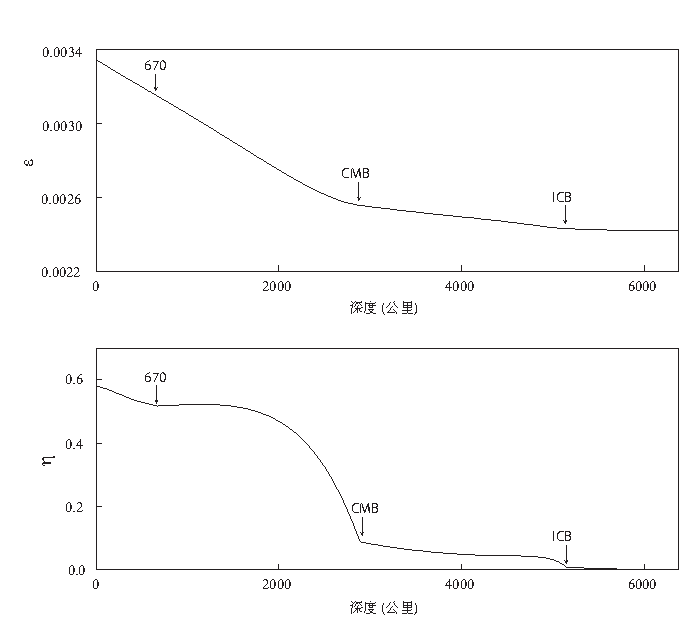
\includegraphics{../figures/chap14/fig01.eps}
\end{center}
\caption[ellipticity]{\label{fig:14.ellipticity}
\iffalse
Depth dependence of the hydrostatic ellipticity $\varepsilon$ ({\em top})
and its logarithmic derivative
$\eta=r\dot{\varepsilon}/\varepsilon$ ({\em bottom})
within the PREM model.  The locations of the 670 km discontinuity,
the core-mantle boundary (CMB) and the inner-core boundary (ICB)
are indicated.
\fi
%%%
PREM~模型的流体静力学椭率~$\varepsilon$~(上图)及其对数导数~$\eta=r\dot{\varepsilon}/\varepsilon$~(下图)的深度依赖性。图中标记了~670~km~处不连续面、核幔边界(CMB)和内核边界(ICB)的位置。
%%%
}
\end{figure}

%\subsection{Mass and moments of inertia}
\subsection{质量和惯性矩}
\index{mass|(}%
\index{moment of inertia|(}%

\iffalse
The mass of a hydrostatically flattened Earth model is the
same as that of the undeformed sphere:
\fi
%%%
流体静力学扁平地球模型的质量与未变形球体的质量相同:
%%%
\eq
M=4\pi\int_0^a\rho\,r^2dr.
\en
\iffalse
The polar and equatorial moments of inertia are given, respectively, by
\fi
%%%
极惯性矩和赤道惯性矩可分别表示为
%%%
\eq
C=\eightthirds\pi\left[\int_0^a\rho\,r^4dr
+\twofifteenth\int_0^a\rho\eps(\eta+5)\,r^4dr\right],
\en
\eq
A=\eightthirds\pi\left[\int_0^a\rho\,r^4dr
-\fifteenth\int_0^a\rho\eps(\eta+5)\,r^4dr\right].
\en
\iffalse
The mean $I=\third(C+2A)$ of the polar and equatorial moments
of inertia is equal to the unperturbed moment of
inertia~(\ref{14.momindef}), as expected.
The {\em precessional constant\/}
\index{precessional constant}%
or so-called dynamical
ellipticity, is the ratio
\fi
%%%
与预期一样,极惯性矩和赤道惯性矩的平均值~$I=\third(C+2A)$~等于未扰动惯性矩~(\ref{14.momindef})~式。进动常数或所谓的动态椭率是如下比值
%%%
\index{dynamical ellipticity}%
\index{ellipticity!dynamical}%
\eq
H=\frac{C-A}{C}=\frac{\fifth\displaystyle{\int_0^a\rho\eps(\eta+5)\,r^4dr}}
{\displaystyle{\int_0^a\rho\,r^4dr}+\twofifteenth
\displaystyle{\int_0^a\rho\eps(\eta+5)\,r^4dr}}.
\en
\iffalse
The hydrostatic value of the precessional constant for any model
having the observed mean radius, mass and moment of inertia of
the Earth is
\fi
%%%
对于具有地球观测平均半径、质量和惯性矩的任意模型,其进动常数的流体静力学值为
%%%
\eq \label{14.Hhydro}
H^{\rm hyd}=1/308.8.
\en
\iffalse
The actual value determined from astronomical observations of
the rate of precession of the equinoxes is one percent higher
(Kinoshita \citeyear{kinoshita77}; Seidelmann \citeyear{seidelmann82};
Williams \citeyear{williams94}):
\fi
%%%
根据二分点进动率的天文观测所确定的实际值比该结果高百分之一(Kinoshita \citeyear{kinoshita77}; Seidelmann \citeyear{seidelmann82}; Williams \citeyear{williams94}):
%%%
\eq \label{14.Hobs}
H^{\rm obs}=1/305.4.
\en
\iffalse
Both of the geodetic discrepancies~(\ref{14.hydreps})--(\ref{14.besteps})
and~(\ref{14.Hhydro})--(\ref{14.Hobs}) are measures of the
degree-two deviation of the density and shape of the Earth
away from hydrostatic equilibrium (Defraigne \citeyear{defraigne97}).
\fi
%%%
两个大地测量差异~(\ref{14.hydreps})--(\ref{14.besteps})~和~(\ref{14.Hhydro})--(\ref{14.Hobs})~均可度量地球密度和形状相对于流体静力学平衡的二阶偏差(Defraigne \citeyear{defraigne97})。
%%%
\index{mass|)}%
\index{moment of inertia|)}%

%\subsection{Elasticity variations}
\subsection{弹性变化}

\iffalse
The results~(\ref{14.ellipticity})--(\ref{14.surfell})
describe the flattening of the surfaces of constant
density and geopotential; strictly speaking, there is no
fundamental reason why they should pertain to the surfaces
of constant incompressibility and rigidity. It is conventional
simply to {\em assume\/} that these elastic level surfaces
{\em coincide\/} with those of the density and geopotential.
Relinquishing our temporary notation, we may then write the
complete catalogue of first-order ellipsoidal perturbations 
in the form
\fi
%%%
(\ref{14.ellipticity})--(\ref{14.surfell})~式描述了等密度面和等重力势面的扁率;严格来说,没有根本的理由说明它们为什么应该属于恒定不可压缩性面和刚性面。传统的做法是简单地假定这些弹性水平面与等密度面和等重力势面重合。放弃我们的临时表示法,可将一阶椭球微扰的完整目录写为
%%%
\begin{displaymath}
\delta\hspace{-0.1 mm}\kappa=\twothirds r\eps\dot{\kappa}P_2(\cos\theta),
\qquad\delta\hspace{-0.2 mm}\mu=\twothirds r\eps\dot{\mu}P_2(\cos\theta),
\end{displaymath}
\begin{displaymath}
\delta\hspace{-0.2 mm}\rho=\twothirds r\eps\dot{\rho}P_2(\cos\theta),
\qquad\delta\Phi=\twothirds(r\eps g-\half\Omega^2 r^2)P_2(\cos\theta),
\end{displaymath}
\eq \label{14.ellperts}
\qquad\qquad\qquad
\delta\hspace{-0.1 mm}d=-\twothirds d\eps_{d} P_2(\cos\theta).
\en
\iffalse
Equations~(\ref{14.ellipticity})--(\ref{14.surfell})
and~(\ref{14.ellperts}) will henceforth be regarded as the
definition of a {\em rotating, hydrostatic, ellipsoidal Earth 
model\/}.
\index{Earth model!rotating, hydrostatic, ellipsoidal}%
Any additional aspherical perturbations $\delta\hspace{-0.1 mm}\kappa$,
$\delta\hspace{-0.2 mm}\mu$,  $\delta\hspace{-0.2 mm}\rho$ and
$\delta\hspace{-0.1 mm}d$ will be referred to as elastic
{\em lateral heterogeneity\/}.
\index{lateral heterogeneity}%
\fi
%%%
(\ref{14.ellipticity})--(\ref{14.surfell})~式和~(\ref{14.ellperts})~式此后将被视为有旋、流体静力学椭球地球模型的定义。任何附加的非球形微扰~$\delta\hspace{-0.1 mm}\kappa$、$\delta\hspace{-0.2 mm}\mu$、$\delta\hspace{-0.2 mm}\rho$~和~$\delta\hspace{-0.1 mm}d$~都将被称为弹性横向不均匀性。
%%%

%\subsection{Geographic versus geocentric colatitude}
\subsection{地理余纬与地心余纬}
\index{geographic colatitude|(}%
\index{colatitude!geographic|(}%
\index{colatitude!geocentric|(}%
\index{geocentric colatitude|(}%
\label{section:14.geocen}

\begin{figure}[!b]
\begin{center}
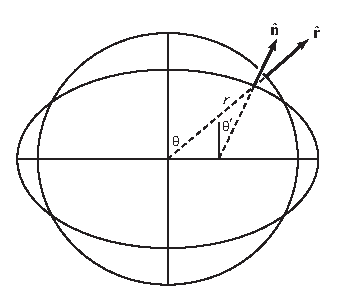
\includegraphics{../figures/chap14/fig02.eps}
\end{center}
\caption[geographic]{\label{fig:14.geographicversusgeocentric}
\iffalse
Cartoon illustrating the relation between the geographical
colatitude $\theta$ and the geocentric colatitude $\theta'$.
The vectors $\hat{\bf n}$ and $\hat{\bf r}$ are the unit
normals to the hydrostatic ellipsoid and the undeformed
(equal-mass) sphere, respectively.
Note that $\theta\geq\theta'$, with equality prevailing
only at the poles and the equator.
\fi
%%%
地理余纬~$\theta$~和地心余纬~$\theta'$~之间的关系示意图。矢量~$\hat{\bf n}$~和~$\hat{\bf r}$~ 分别为流体静力学椭球和未变形(等质量)球体的单位法线。注意~$\theta\geq\theta'$,且只有在两极和赤道面上二者才相等。
%%%
}
\end{figure}
\iffalse
The location of a seismic station situated upon the
Earth's surface is conventionally specified by giving its
elevation $e$ above the geoid, its longitude $\phi$ with
respect to Greenwich, and its {\em geographical colatitude\/}
$\theta'$, which is the angle between the normal $\bnh$ to
the reference ellipsoid and the normal $\bzh$ to the equatorial
plane.  Prior to calculating a synthetic accelerogram or spectrum
by mode summation,
it is necessary to convert the geographic colatitude $\theta'$ to
the corresponding {\em geocentric colatitude\/} $\theta$, which is
the angle between the radius vector $\brh$ and $\bzh$.
Correct to first order in the ellipticity, the two
colatitudes are related by
\fi
%%%
安装在地表的地震台的位置通常是由其在大地水准面以上的高程~$e$、相对格林威治子午线的经度~$\phi$~和地理余纬~$\theta'$(即参考椭球体法线~$\bnh$~与赤道平面法线~$\bzh$~的夹角)来给定。在利用模式叠加计算合成加速度图或谱之前,需要将地理余纬~$\theta'$~转化为地心余纬~$\theta$,后者为径向矢量~$\brh$~与~$\bzh$~的夹角。修正至椭率的一阶项,两个余纬的关系为
%%%
\eq
\tan\theta\approx (1+2\eps_{\rm a})\tan\theta'.
\en
\iffalse
Geometrically, the transformation $\theta'\rightarrow\theta$
projects a point on the reference
ellipsoid to a point on the unperturbed sphere along a line
through the origin.  The original and projected points in
Figure~\ref{fig:14.geographicversusgeocentric} are the feet
of the unit normals $\bnh$ and $\brh$, respectively.
The hypocentral location of an earthquake source is
likewise specified by giving its depth $h$ beneath the
geoid, its longitude $\phi_{\rm s}$ and its geographical
colatitude $\theta^{\prime}_{\rm s}$.  In calculating the
real receiver and source vectors $r_k=\bnuh\cdot\bs_k(\bx)$
and $s_k=\bM\!:\!\beps_k(\bx_{\rm s})$ we stipulate that
\fi
%%%
几何上,$\theta'\rightarrow\theta$~的变换是沿着过原点的直线将参考椭球上的一点投影到未扰动球面上。图~\ref{fig:14.geographicversusgeocentric}~中的原始点和投影点分别是单位法线~$\bnh$~和~$\brh$~的基点。同样,震源的震中位置也是由大地水准面以下的深度~$h$、经度~$\phi_{\rm s}$~和地理余纬~$\theta^{\prime}_{\rm s}$~给定。在计算\textcolor{blue}{实数}接收点矢量~$r_k=\bnuh\cdot\bs_k(\bx)$~和震源矢量~$s_k=\bM\!:\!\beps_k(\bx_{\rm s})$~时,我们规定
%%%
\eq
\bx=(a,\theta,\phi),\qquad\bx_{\rm s}=(a-h,\theta_{\rm s},
\phi_{\rm s}).
\en
\iffalse
A similar geographic-to-geocentric coordinate
transformation must precede the calculation of a
spherical-Earth seismogram or spectrum, using
equations~(\ref{10.DISPUGLY})--(\ref{10.Lorentz}).
Station elevations $e$ are generally ignored
in normal-mode and long-period surface-wave
seismology; however,
they are routinely accounted for in short-period
body-wave travel-time investigations.
\fi
%%%
在采用~(\ref{10.DISPUGLY})--(\ref{10.Lorentz})~式计算球对称地球的地震图或谱图之前,同样需要进行类似的地理到地心坐标转换。在简正模式和长周期面波地震学中,台站高程~$e$~通常被忽略;然而,在短周期体波走时研究中,通常需要考虑它们。
%%%
\index{geographic colatitude|)}%
\index{colatitude!geographic|)}%
\index{colatitude!geocentric|)}%
\index{geocentric colatitude|)}%
\index{ellipticity|)}%
\index{hydrostatic ellipticity|)}%

%\section{Splitting of an Isolated Multiplet}
\section{孤立多重态的分裂}
\index{multiplet!isolated|(}%
\index{isolated multiplet|(}%

\begin{figure}[!b]
\begin{center}
\scalebox{0.92}{
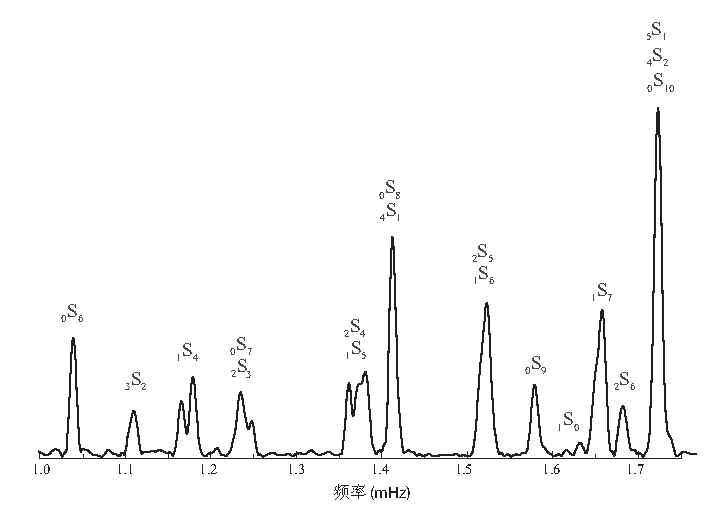
\includegraphics{../figures/chap14/fig03.eps}
}
\end{center}
\caption[lp_spec]{\label{fig:14.lp_spec}
\iffalse
Radial-component, long-period amplitude spectrum
$|\hat{\bf r}\cdot{\bf a}({\bf x},\omega)|$ of the ground acceleration
recorded at station TUC in Tucson, Arizona following
the June 9, 1994 deep-focus Bolivia earthquake.
All of the peaks identified by a single (rather
than double or triple) multiplet
label are well isolated; mode ${}_1{\rm S}_4$
is visibly split.
A Hann taper has been applied to the 80-hour
time series prior to Fourier transformation.
\fi
%%%
1994~年~6~月~9~日玻利维亚深源地震后,亚利桑那州图森~TUC~台站记录的地表径向加速度的长周期振幅谱~$|\hat{\bf r}\cdot{\bf a}({\bf x},\omega)|$。由单一(而非双重或三重)多重态标记识别的所有谱峰均被较好地孤立出来;此外,${}_1{\rm S}_4$~模式发生明显分裂。在进行傅里叶变换之前,对~80~小时时间序列加汉宁窗。
%%%
}
\end{figure}
\iffalse
At long periods several clearly isolated multiplets
may be readily identified in normal-mode spectra,
such as the one illustrated in Figure~\ref{fig:14.lp_spec}.
Shorter-period free oscillations are not as well separated
in frequency; however, a number of high-$Q$ modes may be
successfully isolated by attenuation filtering, as discussed in
Section~10.5.2.  In this section we discuss the splitting
of an isolated multiplet, considering the effects of the
Earth's rotation, hydrostatic ellipticity and lateral
heterogeneity in that order.  For simplicity, we shall
drop the vector and matrix subscripts 0 and 00 used to
denote the target multiplet in Section~\ref{13.sec.isola}.
The elements of the $(2l+1)\times(2l+1)$ self-coupling matrices
are summarized in Appendix~D.4.
\fi
%%%
如图~\ref{fig:14.lp_spec}~所示,在简正模式谱图中的长周期处,可轻易地识别出几个明显的孤立多重态。较短周期的自由振荡在频率上并没有被很好地分离;然而,一些高~$Q$~的模式可通过衰减滤波来成功地孤立出(见~10.5.2~节)。本节我们将讨论孤立多重态的分裂,并依次考虑地球自转、流体静力学椭率和横向不均匀性的影响。为简化起见,我们舍弃~\ref{13.sec.isola}~节中用来表示目标多重态的向量和矩阵下标~0~和~00。附录~D.4~总结了~$(2l+1)\times(2l+1)$~维自耦合矩阵的元素。
%%%

%\subsection{First-order Coriolis splitting}
\subsection{一阶科里奥利分裂}
\index{Coriolis splitting!|(}%
\index{splitting!Coriolis|(}%
\label{section:14.coriolis}

\iffalse
To begin, we consider the first-order effect of the Earth's
rotation, ignoring the centrifugal potential and associated
ellipticity perturbation~(\ref{14.ellperts}).
The splitting is then governed by the $(2l+1)\times(2l+1)$ Coriolis matrix:
$\ssH^{\rm rot}=\ssW$.  This matrix is imaginary and anti-diagonal:
\fi
%%%
首先,我们考虑地球自转的一阶效应,且忽略离心势和相应的椭率微扰~(\ref{14.ellperts})~式。则分裂可由一个~$(2l+1)\times(2l+1)$~维科里奥利矩阵~$\ssH^{\rm rot}=\ssW$~控制。该矩阵是虚数且是反对角阵:
%%%
\eq \label{14.BigW}
\ssH^{\rm rot}=i\chi\Omega\left(\begin{array}{ccccccc}
&&&&&&
\hspace{-3 mm}
\mbox{.\hspace{0.2 ex}\raisebox{.8ex}{.}\hspace{0.2 ex}\raisebox{1.6ex}{.}} \\
&   &&&& \hspace{-3 mm}-m & \\
&&   && \hspace{-2 mm}
\mbox{.\hspace{0.2 ex}\raisebox{.8ex}{.}\hspace{0.2 ex}\raisebox{1.6ex}{.}}
      && \\
&&& \hspace{-2 mm}0 &&& \\
&& \hspace{-2 mm}
\mbox{.\hspace{0.2 ex}\raisebox{.8ex}{.}\hspace{0.2 ex}\raisebox{1.6ex}{.}}
      &&   && \\
& \hspace{-3 mm}m &&&&   & \\
\mbox{.\hspace{0.2 ex}\raisebox{.8ex}{.}\hspace{0.2 ex}\raisebox{1.6ex}{.}}
&&&&&&
\end{array}\right).
\en
\iffalse
The quantity $\chi$ is the {\em Coriolis splitting parameter\/},
\index{Coriolis splitting parameter}%
first given by Backus \& Gilbert (\citeyear{backus&gilbert61}):
\fi
%%%
量~$\chi$~表示科里奥利分裂参数,由~Backus \& Gilbert~(\citeyear{backus&gilbert61})~首次定义:
%%%
\eq \label{14.R}
\chi=k^{-2}\int_0^a\rho(V^2+2kUV+W^2)\,r^2dr,
\en
\iffalse
where $k=\sqrt{l(l+1)}$.
The unitary transformation that diagonalizes~(\ref{14.BigW}) is the
complex-to-real basis transformation, i.e., the Hermitian transpose
of the matrix~(\ref{D.CtoRmat4}):
\fi
%%%
其中,$k=\sqrt{l(l+1)}$。对角化~(\ref{14.BigW})~式的幺正变换是复数基到实数基的变换,也即矩阵~(\ref{D.CtoRmat4})~的厄米特共轭转置:
%%%
\eq
\ssZ^{\rm H}\ssZ=\ssI,\qquad\ssZ^{\rm H}\ssH^{\rm rot}\ssZ=\ssDelta,
\en
\iffalse
where $\ssDelta=\chi\Omega\,{\rm diag}\,
[\,\cdots \,{-m} \,\cdots \,0\, \cdots \, m \, \cdots\,]$ and
\fi
%%%
其中,$\ssDelta=\chi\Omega\,{\rm diag}\,
[\,\cdots \,{-m} \,\cdots \,0\, \cdots \, m \, \cdots\,]$,以及
%%%
\eq \label{14.bigZ}
\ssZ=\left(\begin{array}{ccccccc}
\ddots &&&&&&
\mbox{.\hspace{0.2 ex}\raisebox{.8ex}{.}\hspace{0.2 ex}\raisebox{1.6ex}{.}} \\
& \frac{1}{\sqrt{2}} &&&& \frac{1}{\sqrt{2}} & \\
&& \hspace{-2 mm}-\frac{1}{\sqrt{2}} && \hspace{-2 mm}\frac{1}{\sqrt{2}} && \\
&&& 1 &&& \\
&& \frac{i}{\sqrt{2}} && \frac{i}{\sqrt{2}} && \\
& \hspace{-2 mm}-\frac{i}{\sqrt{2}} &&&& \hspace{-2 mm}\frac{i}{\sqrt{2}} & \\
\mbox{.\hspace{0.2 ex}\raisebox{.8ex}{.}\hspace{0.2 ex}\raisebox{1.6ex}{.}}
&&&&&& \ddots
\end{array}\right).
\en
\iffalse
First-order Coriolis splitting is analogous to the {\em Zeeman
splitting\/}
\index{Zeeman splitting}%
\index{splitting!Zeeman}%
of the quantum energy levels of a hydrogen atom in a
magnetic field; the eigenfrequency perturbations are {\em uniformly
spaced\/}:
\fi
%%%
一阶科里奥利分裂与磁场中氢原子的量子能级的塞曼分裂类似;本征频率微扰是等间距的:
%%%
\eq \label{14.Zeeman}
\delta\om_m=m\chi\Omega,\quad -l\leq m\leq l.
\en
\iffalse
The normalization condition $\int_0^a\rho W^2\,r^2dr=1$ implies that
$\chi=[l(l+1)]^{-1}$ for every toroidal mode ${}_n{\rm T}_l$.  Since the
radial modes ${}_n{\rm S}_0$ are non-degenerate, they are unaffected by the
Coriolis force, correct to first order in $\Omega/\om_0$.
\fi
%%%
对于任意环型模式~${}_n{\rm T}_l$,其归一化条件~$\int_0^a\rho W^2\,r^2dr=1$~意味着~$\chi=[l(l+1)]^{-1}$。精确到~$\Omega/\om_0$~的一阶,由于径向模式~${}_n{\rm S}_0$~是非简并的,因此它们不受科里奥利力的影响。
%%%

\iffalse
The transformed receiver and source vectors~(\ref{13.isol2})--(\ref{13.isol4})
in this approximation are
\fi
%%%
在上述近似下,变换后的接收点与震源矢量~(\ref{13.isol2})--(\ref{13.isol4})~式为:
%%%
\eq
\ssr'=\ssZ^{\rm T}(\ssI-\half\om_0^{-1}\ssW)\ssr,\qquad
\sss'=\ssZ^{\rm H}(\ssI+\half\om_0^{-1}\ssW)\sss,
\en
\iffalse
where we have used the relation $\overline{\ssZ}=\ssZ^*$.
Since $\ssZ$ is the real-to-complex basis transformation
matrix, we find that $\ssr'$ and $\sss'$ are simply related to
the complex-basis receiver and source vectors defined in
Appendix~D.1:
\fi
%%%
其中采用了关系式~$\overline{\ssZ}=\ssZ^*$。由于~$\ssZ$~是实数基到复数基的变换矩阵,因此我们可以看到~$\ssr'$~和~$\sss'$~只与附录~D.1~中定义的复数基接收点矢量和震源矢量有关:
%%%
\eq
\ssr'=(\ssI+\half\om_0^{-1}\ssDelta)\tilde{\ssr}^*,\qquad
\sss'=(\ssI+\half\om_0^{-1}\ssDelta)\tilde{\sss}.
\en
\iffalse
The acceleration response of a rotationally split isolated
multiplet can be written in the form
\fi
%%%
一个旋转分裂的孤立多重态的加速度响应的形式可表示为
%%%
\eq \label{eq:14.acc}
a(t)=\Re{\rm e}_{\,}[A_0(t)\exp(i\omega_0t-\gamma_0t)],
\en
\iffalse
where we have incorporated the effect of spherically
symmetric anelastic attenuation into the unperturbed eigenfrequency
by making the substitution $\omega_0\rightarrow\omega_0+i\gamma_0$.
The slowly varying multiplet modulation function~(\ref{13.target2})
reduces to
\fi
%%%
其中,通过将~$\omega_0$~替换为~$\omega_0\rightarrow\omega_0+i\gamma_0$,我们已将球对称非弹性衰减的影响归并至非扰动本征频率中。此时,慢变多重态调制函数~(\ref{13.target2})~可简化为
%%%
\eq \label{eq:14.A}
A_0(t)=\sum_m[1+m\chi(\Omega/\om_0)]
\tilde{r}_m^*\tilde{s}_m\exp(im\chi\Omega t).
\en
\iffalse
The receiver-source
vector-element product in~(\ref{eq:14.A}) is given explicitly by
\fi
%%%
(\ref{eq:14.A})~式中的接收点—震源矢量的元素积可由下式明确给出
%%%
\eqa \label{14.rmstarsm} \lefteqn{
\tilde{r}_m^*\tilde{s}_m=[\bnuh\cdot\tilde{\bs}_m(\bx)]
[\bM\!:\!\tilde{\beps}_m^*(\bx_{\rm s})]} \nonumber \\
&&\mbox{}\hspace{1.6 mm}=(\bnuh\cdot\bD)
(\bM\!:\!\bE_{\rm s})\hspace{0.4 mm}
Y_{lm}(\theta,\phi)Y_{lm}^*(\theta_{\rm s},\phi_{\rm s}),
\ena
\iffalse
where
\fi
%%%
其中,
%%%
\eq \label{14.dispOp}
\bD=U\brh+k^{-1}V\bdel_1-k^{-1}W(\brh\times\bdel_1),
\en
\eq \label{14.strainOp}
\bE_{\rm s}=\half[\bdel_{\!\rm s}\bD_{\rm s}
+(\bdel_{\!\rm s}\bD_{\rm s})^{\rm T}].
\en
\iffalse
The first-order factor $1+m\chi(\Omega/\om_0)$
insures that the eigenfunctions
are properly orthonormalized with respect to the rotating Earth.
\fi
%%%
一阶因子~$1+m\chi(\Omega/\om_0)$~可确保本征函数相对于有旋地球是完全正交化的。
%%%

\iffalse
Of course, we could have obtained the above results much
more economically by utilizing the complex basis eigenfunctions
$\tilde{\bs}_m$ rather than $\bs_m$ at the outset.  The splitting
matrix in that case would have already been real and diagonal,
\fi
%%%
当然,如果我们从开始就采用复数基本征函数~$\tilde{\bs}_m$~而非~$\bs_m$,可更容易获得上述结果。在这种情况下,分裂矩阵已被复数化和对角化,即
%%%
\eq
\tilde{\ssH}^{\raisebox{-0.45 ex}{\scriptsize\rm rot}}
=\tilde{\ssW}=\ssDelta,
\en
\iffalse
and the unitary transformation matrix $\tilde{\ssZ}$ would have been
the identity.  In quantum-mechanical parlance, the order $-l\leq m\leq l$
of the complex spherical harmonic $Y_{lm}$ is said to be a {\em good quantum
number\/}
\index{good quantum number}%
\index{quantum number!good}%
upon a slowly rotating Earth.
\fi
%%%
且幺正变换矩阵~$\tilde{\ssZ}$~将是单位矩阵。若采用量子力学的说法,复数球谐函数~$Y_{lm}$~的级数~$-l\leq m\leq l$~被称为缓慢旋转地球上的一个好量子数。
%%%

\iffalse
Following Backus \& Gilbert (\citeyear{backus&gilbert61}) we can
obtain an elegant physical interpretation of the result~(\ref{eq:14.A}),
provided we ignore the renormalization factor $1+m\chi(\Omega/\om_0)$.
Substituting~(\ref{14.rmstarsm}) and applying the spherical-harmonic
addition theorem~(\ref{B.addtheor}), we then find that
\fi
%%%
根据~Backus \& Gilbert~(\citeyear{backus&gilbert61}),若忽略重归一化因子~$1+m\chi(\Omega/\om_0)$,我们就可以获得一个关于结果式~(\ref{eq:14.A})~的优雅的物理解释。将~(\ref{14.rmstarsm})~式代入~(\ref{eq:14.A})~式中,并应用球谐加法定理~(\ref{B.addtheor}),可得到
%%%
\eq
A_0(t)=(\bnuh\cdot\bD)(\bM\!:\!\bE_{\rm s})\,P_l[\cos\Theta(t)],
\en
\iffalse
where
$\cos\Theta(t)=\cos\theta\cos\theta_{\rm s}
+\sin\theta\sin\theta_{\rm s}\cos(\phi-\phi_{\rm s}+\chi\Omega t)$.
This differs from the corresponding result upon a non-rotating,
spherical Earth only by the substitution $\Theta\rightarrow\Theta(t)$ or
\fi
%%%
其中~$\cos\Theta(t)=\cos\theta\cos\theta_{\rm s}
+\sin\theta\sin\theta_{\rm s}\cos(\phi-\phi_{\rm s}+\chi\Omega t)$。这与无旋球对称地球的相应结果不同,仅仅只是将~$\Theta$~替换为~$\Theta\rightarrow\Theta(t)$,或者
%%%
\eq
\phi-\phi_{\rm s}\rightarrow\phi-\phi_{\rm s}+\chi\Omega t.
\en
\iffalse
Every multiplet in this approximation has an initial excitation
amplitude $\bA(r,\Theta,\Phi)$ identical to that upon a non-rotating,
spherical Earth; subsequent to the excitation, however, this
pattern {\em rotates westward relative to the Earth at a rate\/}
$\chi\Omega$.  The fastest observed rotation rate is
that of the ${}_0{\rm S}_2$ football mode; its amplitude
pattern $\bA(r,\Theta,\Phi)$ circumnavigates the Earth in
approximately 2.5~days.
\fi
%%%
在上述近似下,每个多重态的初始激发振幅~$\bA(r,\Theta,\Phi)$~都与无旋球对称地球上的相应结果相同;然而,该样式在激发之后将以一定的速度~$\chi\Omega$~相对于地球向西旋转。橄榄球模式~${}_0{\rm S}_2$~的旋转速率是能被最快观测到;其振幅模式~$\bA(r,\Theta,\Phi)$~约~2.5~天可环绕地球一周。
%%%
\index{Coriolis splitting!|)}%
\index{splitting!Coriolis|)}%

%\subsection{Splitting due to rotation and ellipticity}
\subsection{自转和椭率导致的分裂}
\index{splitting!rotation and ellipticity|(}%
\label{section:rotell}

\iffalse
Next, let us consider the combined effects of rotation and
hydrostatic ellipticity.  The $(2l+1)\times(2l+1)$ self-coupling
matrix in this case is of the form
\fi
%%%
接下来,我们考虑自转和流体静力学椭率的联合影响。在这种情况中,$(2l+1)\times(2l+1)$~维自耦合矩阵形式为
%%%
\eq \label{14.rotelleifs}
\ssH^{\rm rot+ell}=\ssW+(2\om_0)^{-1}(\ssV^{\rm ell+cen}-\om_0^2\ssT^{\rm ell}).
\en
\iffalse
Both the kinetic-energy and elliptical-plus-centrifugal
potential-energy matrices are real and diagonal:
\fi
%%%
动能矩阵和椭率加离心势能矩阵均为实数且对角化的,即
%%%
\eq \label{14.Tell}
\ssT^{\rm ell}=\tau\left(\begin{array}{ccccccc}
\ddots &&&&&& \\
& \hspace{-5 mm}1-3m^2/k^2 &&&&& \\
&& \hspace{-10 mm}\ddots &&&& \\
&&& 1 &&& \\
&&&& \ddots && \\
&&&&& \hspace{-5 mm}1-3m^2/k^2 & \\
&&&&&& \hspace{-6 mm}\ddots
\end{array}\right),
\en
\eqa \label{14.Vellcen} \lefteqn{
\ssV^{\rm ell+cen}=\twothirds\Omega^2(1-k^2\chi)\ssI} \nonumber \\
&&\mbox{}
+\upsilon\left(\begin{array}{ccccccc}
\ddots &&&&&& \\
& \hspace{-5 mm}1-3m^2/k^2 &&&&& \\
&& \hspace{-10 mm}\ddots &&&& \\
&&& 1 &&& \\
&&&& \ddots && \\
&&&&& \hspace{-5 mm}1-3m^2/k^2 & \\
&&&&&& \hspace{-6 mm}\ddots
\end{array}\right),
\ena
\iffalse
where
\fi
%%%
其中,
%%%
\eq \label{14.taudef}
\tau=\frac{l(l+1)}{(2l+3)(2l-1)}\int_0^a
\twothirds\eps\rho\bigl[\bar{T}_\rho
-(\eta+3)\check{T}_\rho\bigr]r^2dr,
\en
\eqa \label{14.upsdef} \lefteqn{
\upsilon=\frac{l(l+1)}{(2l+3)(2l-1)}
\int_0^a\twothirds\eps\Bigl\{
\kappa\bigl[\bar{V}_\kappa
-(\eta+1)\check{V}_\kappa\bigr]}
\nonumber \\
&&\mbox{}
+\mu\bigl[\bar{V}_\mu
-(\eta+1)\check{V}_\mu\bigr]
+\rho\bigl[\bar{V}_\rho
-(\eta+3)\check{V}_\rho\bigr]\Bigr\}r^2dr.
\ena
\iffalse
The density, incompressibility and rigidity
kernels $\bar{T}_\rho$, $\check{T}_\rho$
and $\bar{V}_\kappa$, $\check{V}_\kappa$,
$\bar{V}_\mu$, $\check{V}_\mu$, $\bar{V}_\rho$,
$\check{V}_\rho$ are defined in
equations~(\ref{D.selffirst})--(\ref{D.selflast}).
The diagonalizing transformation $\ssZ$ is once again
the real-to-complex basis transformation~(\ref{14.bigZ});
if we had employed the complex basis functions $\tilde{\bs}_m$
instead, the splitting matrix would have been diagonal:
$\tilde{\ssH}^{\raisebox{-0.45 ex}{\scriptsize\rm rot+ell}}
=\ssDelta= {\rm diag}\,[\,\cdots\,\delta\om_m\,\cdots\,]$.
The order $m$ of the complex spherical
harmonic $Y_{lm}$ remains a good quantum number;
however, the linear eigenfrequency perturbations~(\ref{14.Zeeman})
now exhibit a constant and quadratic term:
\fi
%%%
密度、不可压缩性和刚性积分核~$\bar{T}_\rho$、$\check{T}_\rho$~与~$\bar{V}_\kappa$、$\check{V}_\kappa$、$\bar{V}_\mu$、$\check{V}_\mu$、$\bar{V}_\rho$、$\check{V}_\rho$~已被定义在式~(\ref{D.selffirst})--(\ref{D.selflast})~中。对角化变换矩阵~$\ssZ$~同样为实数基至复数基变换~(\ref{14.bigZ})~式;如果我们已采用复数基本征函数~$\tilde{\bs}_m$~替代,分裂矩阵就会是对角化的:$\tilde{\ssH}^{\raisebox{-0.45 ex}{\scriptsize\rm rot+ell}}
=\ssDelta= {\rm diag}\,[\,\cdots\,\delta\om_m\,\cdots\,]$。复数球谐函数~$Y_{lm}$~的级数~$m$~仍然是一个好量子数;然而,线性本征频率微扰公式~(\ref{14.Zeeman})~此时存在一个常数项和一个二次项:
%%%
\eq \label{eq:14.abc}
\delta\omega_m=\omega_0(a+bm+cm^2),\quad -l\leq m\leq l,
\en
\iffalse
where
\fi
%%%
其中,
%%%
\eq \label{14.a}
a=\third(1-k^2\chi)(\Omega/\om_0)^2+\half\om_0^{-2}(\upsilon-\om_0^2\tau),
\en
\eq \label{14.bc}
b=\chi(\Omega/\om_0),\qquad
c=-\threehalves\om_0^{-2}k^{-2}(\upsilon-\om_0^2\tau).
\en
\iffalse
The first term in~(\ref{14.a}) represents
the effect of the spherical part of the centrifugal
potential $\bar{\psi}=\third\Omega^2r^2$, whereas
the second term is due to the combined effects
of the degree-two perturbations $\psi-\bar{\psi}$ and
$\eps$.  Only $\bar{\psi}$ contributes to any shift
in the mean frequency of the multiplet:
\fi
%%%
(\ref{14.a})~式的第一项表示离心势~$\bar{\psi}=\third\Omega^2r^2$~的球形部分影响,而第二项则是来自二阶微扰~$\psi-\bar{\psi}$~和~$\eps$~的联合影响。根据恒等式~$\sum_m
(1-3m^2/k^2)=0$,只有~$\bar{\psi}$~才会导致多重态的平均频率发生一定的频移:
%%%
\eq \label{14.meanell}
\frac{1}{2l+1}\sum_m\delta\om_m=
\third(1-k^2\chi)(\Omega^2\hspace{-0.4 mm}/\om_0),
\en
\iffalse
by virtue of the identity $\sum_m
(1-3m^2/k^2)=0$.  A toroidal multiplet ${}_n{\rm T}_l$
does not exhibit any net shift inasmuch as $\third(1-k^2\chi)=0$.
Every radial-mode eigenfrequency is increased by an amount
$\om_0\rightarrow\om_0[1+\third(\Omega/\omega_0)^2]$.
\fi
%%%
鉴于~$\third(1-k^2\chi)=0$,环型多重态并不会发生任何净频移。每个径向模式的本征频率会增加一个量,即~$\om_0\rightarrow\om_0[1+\third(\Omega/\omega_0)^2]$。
%%%

\iffalse
The acceleration response of an isolated
multiplet upon a rotating, elliptical Earth
is again of the form~(\ref{eq:14.acc}); the
multiplet modulation function~(\ref{eq:14.A})
is generalized to
\fi
%%%
在有旋椭球地球上,一个孤立多重态的加速度响应仍采用~(\ref{eq:14.acc})~式的形式;多重态调制函数~(\ref{eq:14.A})~推广为
%%%
\eqa \label{14.Aell} \lefteqn{
A_0(t)=\sum_m[1+m\chi(\Omega/\om_0)-\tau(1-3m^2\!/k^2)]} \nonumber \\
&&\mbox{}\qquad\qquad\qquad\times
\tilde{r}_m^*\tilde{s}_m\exp[i\omega_0(a+bm+cm^2)t],
\ena
\iffalse
where the term $1+m\chi(\Omega/\om_0)-\tau(1-3m^2\!/k^2)$
arises from the renormalization.  The spectral analogue
of equation~(\ref{14.Aell}) is a superposition of $2l+1$
Lorentzians centered upon the split singlet
eigenfrequencies:
\fi
%%%
式中,$1+m\chi(\Omega/\om_0)-\tau(1-3m^2\!/k^2)$~项来自重归一化。(\ref{14.Aell})~式的频谱形式是~$2l+1$~个以分裂的单态模式本征频率为中心的洛伦兹函数的叠加:
%%%
\eq \label{14.firstspect}
a(\om)=\sum_m[1+m\chi(\Omega/\om_0)-\tau(1-3m^2\!/k^2)]
\tilde{r}_m^*\tilde{s}_m\hspace{0.4 mm}\eta_m(\om),
\en
\iffalse
where $\eta_m=\half[\gamma_0+i(\om-\om_0-\delta\om_m)]^{-1}$.
A radial-component sensor
at the South Pole seismic station SPA has $\tilde{r}_m=0$ for
$m\not=0$.  This results in an {\em unsplit\/} spectrum:
$a(\om)=(1-\tau)\tilde{r}_0^*\tilde{s}_0
\hspace{0.4 mm}\eta_0(\om)$.
\index{splitting!rotation and ellipticity|)}%
\fi
%%%
其中,$\eta_m=\half[\gamma_0+i(\om-\om_0-\delta\om_m)]^{-1}$。南极地震台站~SPA~的径向分量传感器有~$\tilde{r}_m=0$($m\not=0$)。这产生一个无分裂频谱:$a(\om)=(1-\tau)\tilde{r}_0^*\tilde{s}_0
\hspace{0.4 mm}\eta_0(\om)$。
%%%

\renewcommand{\thesubsection}{$\!\!\!\raise1.3ex\hbox{$\star$}\!\!$
\arabic{chapter}.\arabic{section}.\arabic{subsection}}
%\subsection{Second-order Coriolis splitting}
\subsection{二阶科里奥利分裂}
\index{splitting!Coriolis!second-order|(}%
\index{Coriolis splitting!second-order|(}%
\renewcommand{\thesubsection}{\arabic{chapter}.\arabic{section}.\arabic{subsection}}
\label{section:10.second-orderCoriolis}

\iffalse
The Coriolis force exerts a perturbation upon the Earth's free
oscillations of order $\Omega/\omega_0$, whereas the centrifugal
force is a perturbation of order $(\Omega/\omega_0)^2$.  A complete
treatment of the Earth's rotation to order $(\Omega/\omega_0)^2$
must account for the effect of the Coriolis force to {\em second
order\/}.  We present a brief account of the requisite second-order
analysis in this section.  The matrix formulation developed in
Chapter~13 is difficult to extend to higher order; for this reason,
we resort to classical Rayleigh-Schr\"{o}dinger perturbation theory,
following the original treatment of the Coriolis splitting
problem by Backus \& Gilbert (\citeyear{backus&gilbert61}).
\fi
%%%
科里奥利力对地球自由振荡施加一个~$\Omega/\omega_0$~量级的微扰,而离心力则是一个~$(\Omega/\omega_0)^2$~量级的微扰。要完整地考虑地球自转到~$(\Omega/\omega_0)^2$~量级,必须考虑科里奥利力的影响至二阶。在本节中,我们简要介绍必要的二阶分析。由于第~13~章发展的矩阵公式难以推广到更高阶,因此我们采用经典的瑞利--薛定谔微扰理论,并沿用~Backus \& Gilbert~(\citeyear{backus&gilbert61})~对科里奥利分裂问题的最初处理方法。
%%%

\iffalse
Let $\sH$ be the elastic-gravitational operator~(\ref{4.Hhydro})
governing the free oscillations of a spherically symmetric,
non-rotating Earth model.  We denote the real eigenfrequencies
and associated {\em complex\/} eigenfunctions of this
unperturbed Earth model by $\om_k$ and $\tilde{\bs}_k$.
We seek to find perturbed real eigenfrequencies $\om$
and associated complex eigenfunctions $\bu$ which satisfy
the equation
\fi
%%%
令~$\sH$~表示控制球对称、无旋地球模型自由振荡的弹性--重力算子~(\ref{4.Hhydro})~式,用~$\om_k$~和~$\tilde{\bs}_k$~表示该未扰动地球模型的实本征频率和相应的复本征函数。我们尝试寻求满足如下方程的扰动实本征频率~$\om$~及其相应复本征函数~$\bu$
%%%
\eq \label{14.DS1}
\sH\bu+2i\om\Omega_{\,}\bzh\times\bu=\om^2\bu.
\en
\iffalse
We look for ordinary perturbative solutions to~(\ref{14.DS1})
of the form
\fi
%%%
\textcolor{blue}{我们寻找方程~(\ref{14.DS1})~的常微扰解形式为:}
%%%
\eq \label{14.DS2}
\om/\om_0=1+\xi_1(\Omega/\om_0)+\xi_2(\Omega/\om_0)^2+\cdots,
\en
\eq \label{14.DS3}
\bu=\bu_0+\bu_1(\Omega/\om_0)+\bu_2(\Omega/\om_0)^2+\cdots,
\en
\iffalse
where the expansion parameter $\Omega/\om_0$
is presumed to be small.
Inserting~(\ref{14.DS2})--(\ref{14.DS3}) into~(\ref{14.DS1})
and equating powers of $\Omega/\om_0$, we obtain a sequence
of equations, of which we write only the first three:
\fi
%%%
其中,展开参数~$\Omega/\om_0$~被假设为小量。将~(\ref{14.DS2})--(\ref{14.DS3})~式代入~(\ref{14.DS1})~式中,并使其等于~$\Omega/\om_0$~的幂,由此可得到了一系列方程,此处只写出其中的前三个:
%%%
\eq \label{14.DS4}
(\sH-\om_0^2)\bu_0=\bzero,
\en
\eq \label{14.DS5}
(\sH-\om_0^2)\bu_1=2\om_0^2(\xi_1\bu_0-i\bzh\times\bu_0)\equiv\be_1,
\en
\vspace{-3.0 mm}
\eqa \label{14.DS6} \lefteqn{
(\sH-\om_0^2)\bu_2=2\om_0^2(\xi_1\bu_1-i\bzh\times\bu_1)} \nonumber \\
&&\mbox{}+2\om_0^2\xi_1(\xi_1\bu_0-i\bzh\times\bu_0)
+\om_0^2(2\xi_2-\xi_1^2)\bu_0\equiv\be_2.
\ena
\iffalse
The zeroth-order equation~(\ref{14.DS4}) simply states that $\om_0$
and $\bu_0$ must be an eigenfrequency and associated eigenfunction
of the unperturbed, non-rotating Earth model.  Knowing that the order
$m$ of $Y_{lm}$ is a good quantum number, we take the zeroth-order
eigenfunction to be a {\em single\/} complex basis eigenfunction:
\fi
%%%
零阶方程~(\ref{14.DS4})~简要描述了~$\om_0$~和~$\bu_0$~必须是无扰动、无旋地球模型的本征频率和相应本征函数。已知~$Y_{lm}$~的级数~$m$~是一个好量子数,我们取零阶本征函数为一个单独的复基本征函数:
%%%
\eq \label{14.DSextra}
\bu_0=\tilde{\bs}_0.
\en
\iffalse
The choice~(\ref{14.DSextra}) is advantageous, since it allows
us to proceed with an essentially {\em non-degenerate\/} version
of perturbation theory.  We employ the complex inner product
$\langle\bs,\bs'\rangle=\int_{\subearth}\rho\hspace{0.3 mm}
\bs^*\cdot\bs'\,dV$ introduced in equation~(\ref{4.inprod2}).
Orthogonality $\langle\bs,\bs'\rangle=0$ of two complex
functions will be indicated by the notation $\bs\perp\bs'$.
Since the normalization of $\bu$ is at our disposal,
we may without loss of generality require that
$\bu_k\perp\tilde{\bs}_0$ for $k\not=0$.
\fi
%%%
选择~(\ref{14.DSextra})~式是有利的,因为它允许我们继续处理微扰理论的本质上的非简并版本。我们利用在~(\ref{4.inprod2})~式中介绍的复内积~$\langle\bs,\bs'\rangle=\int_{\subearth}\rho\hspace{0.3 mm}
\bs^*\cdot\bs'\,dV$。两个复函数的正交性~$\langle\bs,\bs'\rangle=0$~可采用符号~$\bs\perp\bs'$~表示。由于处理过程中考虑了~$\bu$~的归一化,因此我们要求~$\bu_k\perp\tilde{\bs}_0$($k\not=0$),且不失普适性。
%%%

\iffalse
The Hermitian character of the operator
$\sH$ assures us that~(\ref{14.DS5})
has a unique solution $\bu_1\perp\tilde{\bs}_0$
if and only if $\be_1\perp\tilde{\bs}_0$, and that~(\ref{14.DS6})
has a unique solution $\bu_2\perp\tilde{\bs}_0$
if and only if $\be_2\perp\tilde{\bs}_0$.
The first of these solubility conditions
determines the first-order Coriolis splitting
parameter:
\fi
%%%
算符~$\sH$~的厄米特性质保证了~(\ref{14.DS5})~式当且仅当~$\be_1\perp\tilde{\bs}_0$~时有唯一解~$\bu_1\perp\tilde{\bs}_0$;而~(\ref{14.DS6})~式当且仅当~$\be_2\perp\tilde{\bs}_0$~时有唯一解~$\bu_2\perp\tilde{\bs}_0$。\textcolor{red}{这些可溶性条件的第一个}决定了一阶科里奥利分裂参数:
%%%
\eq \label{14.DS7}
\xi_1=\int_{\subearth}\rho\hspace{0.3 mm}\tilde{\bs}_0^*
\cdot(i\bzh\times\tilde{\bs}_0)\,dV.
\en
\iffalse
Evaluation of the integral~(\ref{14.DS7}) yields the
previous result $\xi_1=m\chi$, as expected.
The second condition reduces to
\fi
%%%
如预期的,对积分式~(\ref{14.DS7})~的计算可得到上述结果~$\xi_1=m\chi$。第二个条件简化为
%%%
\eq \label{14.DS8}
2\xi_2-\xi_1^2=2\int_{\subearth}\rho\hspace{0.3 mm}
\bu_1^*\cdot(i\bzh\times\tilde{\bs}_0)\,dV.
\en
\iffalse
As usual in Rayleigh-Schr\"{o}dinger perturbation theory,
\index{Rayleigh-Schr\"{o}dinger perturbation theory}%
we must solve for the first-order correction to the
eigenfunction $\bu_1$ before we can find the
second-order correction to the eigenfrequency $\xi_2$.
Since $\bu_1\perp\tilde{\bs}_0$, we may expand it
in terms of all of the other unperturbed basis
eigenfunctions:
\fi
%%%
与瑞利--薛定谔微扰理论中的通常做法一样,在我们能找到本征频率~$\xi_2$~的二阶修正之前,必须先求出本征函数~$\bu_1$~的一阶修正。由于~$\bu_1\perp\tilde{\bs}_0$,可采用其他所有非扰动基本征函数对其进行展开,即
%%%
\eq \label{14.DS9}
\bu_1=\sum_{k\not=0}\langle\tilde{\bs}_k,\bu_1\rangle
\hspace{0.3 mm}\tilde{\bs}_k.
\en
\begin{table}[!b]
\centering
\label{table:14.abc}
\begin{tabular}{|c|r|r|r||c|r|r|r|} \hline
     &     &     &     &     &     &    & \\
Mode & $a$\hspace{4.5 mm} & $b$\hspace{4.0 mm} & $c$\hspace{5.0 mm} &
Mode & $a$\hspace{4.0 mm} & $b$\hspace{4.0 mm} & $c$\hspace{5.0 mm} \\
     &     &     &     &     &     &     & \\ \hline
     &     &     &     &     &     &     & \\
${}_{0}{\rm T}_{2}$ &  $-1.335$ &   5.090 &  $-0.231$ &
${}_{1}{\rm S}_{1}$ &   15.306 &   98.380 &  $-0.554$ \\
${}_{0}{\rm T}_{3}$ &   0.558 &   1.647 &  $-0.279$ &
${}_{1}{\rm S}_{2}$ &   1.177 &   4.173 &  $-0.428$ \\
${}_{0}{\rm T}_{4}$ &   0.849 &   0.757 &  $-0.162$ &
${}_{1}{\rm S}_{3}$ &   0.922 &   2.633 &  $-0.215$ \\
${}_{0}{\rm T}_{5}$ &   0.917 &   0.416 &  $-0.102$ &
${}_{1}{\rm S}_{4}$ &   0.795 &   1.948 &  $-0.122$ \\
${}_{0}{\rm T}_{6}$ &   0.923 &   0.256 &  $-0.069$ &
${}_{1}{\rm S}_{5}$ &   0.696 &   1.437 &  $-0.075$ \\
${}_{0}{\rm T}_{7}$ &   0.926 &   0.170 &  $-0.050$ &
${}_{1}{\rm S}_{6}$ &   0.618 &   0.873 &  $-0.049$ \\
${}_{0}{\rm T}_{8}$ &   0.961 &   0.119 &  $-0.038$ &
${}_{1}{\rm S}_{7}$ &   0.561 &   0.564 &  $-0.033$ \\
     &     &     &    &
${}_{1}{\rm S}_{8}$ &   0.500 &   0.427 &  $-0.023$ \\
${}_{1}{\rm T}_{1}$ &  $-0.604$ &   4.687 &   0.897 &
${}_{1}{\rm S}_{9}$ &   0.446 &   0.349 &  $-0.017$ \\
${}_{1}{\rm T}_{2}$ &   0.250 &   1.463 &  $-0.156$ &
     &     &     &     \\
${}_{1}{\rm T}_{3}$ &   0.517 &   0.671 &  $-0.128$ &
${}_{2}{\rm S}_{3}$ &   0.662 &   0.668 &  $-0.153$ \\
${}_{1}{\rm T}_{4}$ &   0.576 &   0.366 &  $-0.084$ &
${}_{2}{\rm S}_{4}$ &   0.659 &   0.281 &  $-0.093$ \\
${}_{1}{\rm T}_{5}$ &   0.599 &   0.221 &  $-0.058$ &
${}_{2}{\rm S}_{5}$ &   0.681 &   0.159 &  $-0.064$ \\
${}_{1}{\rm T}_{6}$ &   0.616 &   0.143 &  $-0.042$ &
${}_{2}{\rm S}_{6}$ &   0.690 &   0.340 &  $-0.047$ \\
     &     &     &     &     &     &     & \\
${}_{2}{\rm T}_{2}$ &   0.413 &   0.866 &  $-0.207$ &
${}_{3}{\rm S}_{1}$ &   0.413 &   1.657 &  $-0.353$ \\
${}_{2}{\rm T}_{3}$ &   0.565 &   0.421 &  $-0.141$ &
${}_{3}{\rm S}_{2}$ &   0.652 &   1.485 &  $-0.292$ \\
     &     &     &     &     &     &     & \\
${}_{0}{\rm S}_{0}$ &   0.336 &   0.000 &   0.000 &
${}_{6}{\rm S}_{3}$ &   0.548 &   $-0.050$ &  $-0.136$ \\
${}_{1}{\rm S}_{0}$ &   0.094 &   0.000 &   0.000 &
${}_{8}{\rm S}_{1}$ &   0.893 &    0.081 &  $-1.332$ \\
     &     &     &    &
${}_{8}{\rm S}_{5}$ &   0.591 &    0.019 &  $-0.059$ \\
${}_{0}{\rm S}_{2}$ &   0.376 &  14.905 &  $-0.267$ &
${}_{9}{\rm S}_{3}$ &   0.626 &    0.055 &  $-0.156$ \\
${}_{0}{\rm S}_{3}$ &   0.463 &   4.621 &  $-0.118$ &
${}_{11}{\rm S}_{4}$ &   0.587 &   0.013 &  $-0.088$ \\
${}_{0}{\rm S}_{4}$ &   0.544 &   1.834 &  $-0.075$ &
${}_{11}{\rm S}_{5}$ &   0.585 &   0.005 &  $-0.058$ \\
${}_{0}{\rm S}_{5}$ &   0.452 &   0.841 &  $-0.047$ &
${}_{13}{\rm S}_{1}$ &   0.884 &    0.102 &  $-1.323$ \\
${}_{0}{\rm S}_{6}$ &   0.391 &   0.407 &  $-0.033$ &
${}_{13}{\rm S}_{2}$ &   0.659 &    0.031 &  $-0.329$ \\
${}_{0}{\rm S}_{7}$ &   0.354 &   0.181 &  $-0.025$ &
${}_{18}{\rm S}_{3}$ &   0.604 &   0.020 &  $-0.151$ \\
${}_{0}{\rm S}_{8}$ &   0.273 &   0.064 &  $-0.020$ &
${}_{18}{\rm S}_{4}$ &   0.590 &   0.017 &  $-0.088$ \\
     &     &     &     &     &     &     & \\ \hline
\end{tabular}
\caption[splitting coeffs]{
\iffalse
Rotational and elliptical splitting parameters
for selected toroidal and spheroidal
modes of Earth model 1066A (Gilbert \& Dziewonski
\protect\citeyear{gilbert&dziewonski75}).
The parameters $a$ and $c$ incorporate the second-order
Coriolis corrections of \protect\textcite{dahlen&sailor79}.
All of the tabulated values must be multiplied by $10^{-3}$.
\fi
%%%
1066A~地球模型(Gilbert \& Dziewonski~\protect\citeyear{gilbert&dziewonski75})的部分环型和球型模式的自转和椭率分裂参数。参数~$a$~和~$c$~包含~Dahlen \& Sailor~\protect\textcite{dahlen&sailor79}~的二阶科里奥利改正。所有列表值需乘以~$10^{-3}$
%%%
}
\end{table}
\iffalse
To find the expansion coefficients $\langle\tilde{\bs}_k,\bu_1\rangle$,
we substitute~(\ref{14.DS9}) into equation~(\ref{14.DS5}) and make use
of the orthonormality $\langle\tilde{\bs}_k,\tilde{\bs}_{k'}\rangle=
\delta_{kk'}$.  This leads to the relation
\fi
%%%
为求展开系数~$\langle\tilde{\bs}_k,\bu_1\rangle$,将式~(\ref{14.DS9})~代入式~(\ref{14.DS5})~中,并利用归一正交性~$\langle\tilde{\bs}_k,\tilde{\bs}_{k'}\rangle=
\delta_{kk'}$,可得到如下关系
%%%
\eq \label{14.DS10}
\langle\tilde{\bs}_k,\bu_1\rangle=\frac{2\om_0^2}{\om_0^2-\om_k^2}
\int_{\subearth}\rho\hspace{0.3 mm}\tilde{\bs}_k^*\cdot(i\bOmega\times
\tilde{\bs}_0)\,dV.
\en
\iffalse
Upon substituting~(\ref{14.DS9})--(\ref{14.DS10}) into
equation~(\ref{14.DS8}), we obtain an explicit expression
for the second-order Coriolis splitting parameter:
\fi
%%%
将式~(\ref{14.DS9})--(\ref{14.DS10})~代入式~(\ref{14.DS8})~中,可得到二阶科里奥利分裂参数的显式表达式:
%%%
\eq \label{14.DSfin}
2\xi_2-\xi_1^2=4\sum_{k\not=0}\frac{\om_0^2}{\om_0^2-\om_k^2}
\left|\int_{\subearth}\rho\hspace{0.3 mm}\tilde{\bs}_k^*\cdot
(i\bOmega\times\tilde{\bs}_0)\,dV\right|^2.
\en
\iffalse
Most of the terms in the sums~(\ref{14.DS9}) and~(\ref{14.DSfin})
are zero, by virtue of the orthogonality of the basis eigenfunctions
$\tilde{\bs}_k$.  In fact, correct to first order in $\Omega/\om_0$,
a toroidal multiplet ${}_n{\rm T}_l$ is only coupled to the adjacent
spheroidal multiplets ${}_{n'}{\rm S}_{l\pm 1}$, whereas a spheroidal
multiplet ${}_n{\rm S}_l$ is coupled to the adjacent toroidal multiplets
${}_{n'}{\rm T}_{l\pm 1}$ and the adjacent spheroidal multiplets
${}_{n'}{\rm S}_l,\,n'\not= n$.  To insure completeness, it
is necessary to include absolutely
all of the possible coupling partners, including
the rigid-body and geostrophic trivial modes discussed in Sections~8.7.2
and~8.8.2.  A detailed recipe for evaluating the sum~(\ref{14.DSfin}) is
given by Dahlen \& Sailor (\citeyear{dahlen&sailor79}).  The final
second-order splitting parameter consists of a constant plus a quadratic
term:
\fi
%%%
由于基本征函数~$\tilde{\bs}_k$~的正交性,(\ref{14.DS9})~式和~(\ref{14.DSfin})~式的大部分求和项为零。事实上,精确到~$\Omega/\om_0$~的一阶,环型多重态~${}_n{\rm T}_l$~只与其邻近的球型多重态~${}_{n'}{\rm S}_{l\pm 1}$~发生耦合,而球型多重态~${}_n{\rm S}_l$~只与其邻近的环型多重态${}_{n'}{\rm T}_{l\pm 1}$ 和球型多重态~${}_{n'}{\rm S}_l,\,n'\not= n$( )发生耦合。为确保完整性,有必要包含所有可能的耦合部分,包括~8.7.2~和~8.8.2~节中讨论的刚体和地转微小模式。Dahlen \& Sailor~(\citeyear{dahlen&sailor79})~给出了计算求和式~(\ref{14.DSfin})~的详细方法。最终的二阶分裂参数包含一个常数项加上一个二次项:
%%%
\eq \label{14.Coriolis2}
\xi_2=\lambda+m^2\zeta.
\en
\iffalse
The upshot is that the eigenfrequency perturbations $\delta\om_m$ are still of
the form~(\ref{eq:14.abc}), with modified values of the coefficients:
\fi
%%%
其结果是,本征频率微扰~$\delta\om_m$~仍然是式~(\ref{eq:14.abc})~的形式,其系数的修改值为:
%%%
\eq \label{14.Coriolis2p}
a\rightarrow a+\lambda(\Omega/\om_0)^2,\qquad
c\rightarrow c+\zeta(\Omega/\om_0)^2.
\en
\iffalse
With the modification~(\ref{14.Coriolis2p}),
the result~(\ref{14.Aell}) is correct
to first order in the ellipticity and second order in the rotation.
In Table~14.1 we list the splitting parameters $a$, $b$ and $c$, 
for a number of moderately well-isolated toroidal and spheroidal
multiplets of interest.  The second-order Coriolis corrections
are significant for several of the Earth's gravest observed modes,
including the fundamental toroidal, spheroidal and radial modes
${}_0{\rm T}_2$, ${}_0{\rm S}_2$ and ${}_0{\rm S}_0$.  Note that
the as-yet-undetected Slichter triplet ${}_1{\rm S}_1$ is predicted
to be severely split by the first-order Coriolis force.
\fi
%%%
经过式~(\ref{14.Coriolis2p})~的修改,结果式~(\ref{14.Aell})~在椭率上是一阶的,在自转上是二阶的。表~14.1~列出了一些适度孤立的环型和球型多重态的分裂参数~$a$、$b$~和~$c$。二阶科里奥利修正对于几个地球\textcolor{red}{最重要}观测模式都很重要,包括基阶环型模式~${}_0{\rm T}_2$、基阶球型模式~${}_0{\rm S}_2$~和基阶径向模式~${}_0{\rm S}_0$。值得注意的是,目前尚未检测到的~Slichter~模三重分裂模式~${}_1{\rm S}_1$~预计将被一阶科里奥利力严重分裂。
%%%
\index{Slichter mode}%
\index{mode!Slichter}%
\index{splitting!Coriolis!second-order|)}%
\index{Coriolis splitting!second-order|)}%

%\subsection{Effect of lateral heterogeneity}
\subsection{横向不均匀性的影响}
\index{splitting!lateral heterogeneity|(}%

\iffalse
The Earth's hydrostatic equatorial bulge is the most
visible manifestation of its asphericity.  Many low-frequency
multiplets are, however, much more strongly split by non-hydrostatic
{\em lateral heterogeneity\/}.  These additional perturbations
\index{lateral heterogeneity}%
can be expanded in real surface spherical harmonics $\sY_{lm}$
in the form
\fi
%%%
地球的流体静力学赤道隆起是其非球面性的最明显表现。然而,许多低频多重态被非流体静力学横向不均匀性分裂得更强烈。这些附加微扰可利用实数球谐函数~$\sY_{lm}$~展开为
%%%
\begin{displaymath}
\delta\hspace{-0.1 mm}\kappa=\sum_{s=1}^{s_{\rm max}}
\sum_{t=-s}^s\delta\hspace{-0.1 mm}\kappa_{st}\sY_{st},\qquad
\delta\hspace{-0.2 mm}\mu=\sum_{s=1}^{s_{\rm max}}
\sum_{t=-s}^s\delta\hspace{-0.2 mm}\mu_{st}\sY_{st},
\end{displaymath}
\begin{displaymath}
\delta\hspace{-0.3 mm}\rho=\sum_{s=1}^{s_{\rm max}}
\sum_{t=-s}^s\delta\hspace{-0.3 mm}\rho_{st}\sY_{st},\qquad
\delta\Phi=\sum_{s=1}^{s_{\rm max}}
\sum_{t=-s}^s\delta\Phi_{st}\sY_{st},
\end{displaymath}
\eq \label{14.latperts}
\qquad\qquad\qquad
\delta\hspace{-0.1 mm}d=\sum_{s=1}^{s_{\rm max}}
\sum_{t=-s}^s\delta\hspace{-0.1 mm}d_{st}\sY_{st}.
\en
\iffalse
The sums in~(\ref{14.latperts}) commence at $s=1$ because
of our presumption that the unperturbed Earth model is the
terrestrial monopole.  In forward-modelling applications
the maximum degree $s_{\rm max}$ is limited only by computer
storage considerations; in inversion studies, it is
governed by the resolution of the available dataset.
Ignoring the Earth's rotation and ellipticity for the moment,
we shall denote the splitting matrix due to lateral heterogeneity
alone by
\fi
%%%
(\ref{14.latperts})~式中的求和计算是从~$s=1$~开始的,因为我们假定未扰动地球模型是地球单极子。在正演应用中,最大阶数~$s_{\rm max}$~仅受计算机存储的限制;在反演研究中,它取决于可用数据集的分辨率。暂时忽略地球的自转和椭率,将仅由横向不均匀性导致的分裂矩阵表示为
%%%
\eq \label{14.lathet}
\ssH^{\rm lat}=(2\om_0)^{-1}(\ssV^{\rm lat}-\om_0^2\ssT^{\rm lat}).
\en
\iffalse
The real elements of~(\ref{14.lathet}) may be written in the form
\fi
%%%
(\ref{14.lathet})~式的实数元素可以写成如下形式
%%%
\eq \label{14.Gaunt}
H_{mm'}^{\rm lat}=\omega_0\sum_{st}\sigma_{st}
\int_{\Omega}\sY_{lm}\sY_{st}\sY_{lm'}\,d\Omega,
\en
\iffalse
where
\fi
%%%
其中,
%%%
\eqa \label{eq:14.cst}
\lefteqn{
\sigma_{st}=\half\omega_0^{-2}\biggl\{\int_0^a
[\delta\hspace{-0.1mm}\kappa_{st}V_\kappa+\delta\hspace{-0.2mm}\mu_{st}V_\mu
+\delta\hspace{-0.2mm}\rho_{st}(V_\rho-\omega_0^2T_\rho)]\,r^2dr
} \nonumber \\
&&\mbox{}
+\sum_d d^2\delta\hspace{-0.1mm}d_{st}[V_d-\omega_0^2T_d]_-^+\biggr\}.
\ena
\iffalse
Explicit expressions for the quantities $V_\kappa$, $V_\mu$,
$V_\rho-\om_0^2T_\rho$ and $V_d-\om_0^2T_d$ may be found
in Appendix~D.4.2.  These kernels depend
upon the degree $s$ of the heterogeneity; however, they are
independent of the order $t$.  It is evident that the matrix $\ssH^{\rm lat}$
is real and symmetric: $H^{\rm lat}_{mm'}=H^{\rm lat}_{m'm}$.
The real {\em Gaunt integrals\/}
\index{Gaunt integral}%
in equation~(\ref{14.Gaunt}) satisfy
the {\em selection rules\/}
\fi
%%%
$V_\kappa$、$V_\mu$、$V_\rho-\om_0^2T_\rho$~和~$V_d-\om_0^2T_d$~的显式表达式可参见附录~D.4.2。这些积分核函数取决于不均匀性的次数~$s$,而与阶数~$t$~无关。显然,矩阵~$\ssH^{\rm lat}$~是实数且对称的,即~$H^{\rm lat}_{mm'}=H^{\rm lat}_{m'm}$。(\ref{14.Gaunt})~式中的实数冈特积分满足选择法则
%%%
\index{selection rules}%
\index{angular selection rules}%
\eq \label{14.selrule}
\int_{\Omega}\sY_{lm}\sY_{st}\sY_{lm'}\,d\Omega=0\quad
\mbox{unless}\!\!\quad\left\{\begin{array}{l}
\mbox{$s$ is even} \\ 0\leq s\leq 2l \\ t=m-m'.
\end{array}\right.
\en
\iffalse
The first rule stipulates that {\em the splitting of an isolated multiplet
depends only upon the even-degree structure of the Earth\/}.  This
\index{even-degree structure}%
obviously
has important implications for the lateral-heterogeneity inverse problem.
\fi
%%%
第一条法则规定,孤立多重态的分裂只取决于地球的偶数阶结构。这显然对横向不均匀性的反演问题具有重要意义。
%%%

\iffalse
Lateral variations in anelasticity may be easily incorporated
by allowing the incompressibility and rigidity to be complex:
$\delta\hspace{-0.1 mm}\kappa\rightarrow\delta\hspace{-0.1 mm}\kappa
+i\kappa_0q_{\kappa}$ and $\delta\hspace{-0.2 mm}\mu\rightarrow
\delta\hspace{-0.2 mm}\mu+i\kappa_0q_{\mu}$, where
\fi
%%%
通过允许不可压缩性和刚性为复数,可轻易地把非弹性的横向变化包括进来,即~$\delta\hspace{-0.1 mm}\kappa\rightarrow\delta\hspace{-0.1 mm}\kappa
+i\kappa_0q_{\kappa}$~和~$\delta\hspace{-0.2 mm}\mu\rightarrow
\delta\hspace{-0.2 mm}\mu+i\kappa_0q_{\mu}$,其中,
%%%
\eq
q_{\kappa}=\sum_{s=1}^{s_{\rm max}}
\sum_{t=-s}^sq_{\kappa st}\sY_{st},\qquad
q_{\mu}=\sum_{s=1}^{s_{\rm max}}
\sum_{t=-s}^sq_{\mu st}\sY_{st}.
\en
\iffalse
The splitting matrix~(\ref{14.lathet}) is generalized to
\fi
%%%
将分裂矩阵~(\ref{14.lathet})~式推广为
%%%
\eq \label{14.alathet}
\ssH^{\rm lat}=(2\om_0)^{-1}(\ssV^{\rm lat}+i\ssA-\om_0^2\ssT^{\rm lat}).
\en
\iffalse
The elements of the anelastic perturbation matrix $\ssA$ are given by
\fi
%%%
非弹性微扰矩阵~$\ssA$~的元素可表示为
%%%
\eq \label{eq:14.Ael}
A_{mm'}=\omega_0\sum_{st}\psi_{st}
\int_{\Omega}\sY_{lm}\sY_{st}\sY_{lm'}\,d\Omega,
\en
\iffalse
where
\fi
%%%
其中,
%%%
\eq \label{eq:14.ast}
\psi_{st}=\half\omega_0^{-2}\int_0^a(\kappa_0q_{\kappa st}
V_\kappa+\mu_0q_{\mu st}V_\mu)\,r^2dr.
\en
\iffalse
In this case $\ssH^{\rm lat}$ is complex symmetric; the
selection rules~(\ref{14.selrule}) are again applicable,
so that there is no dependence of the splitting upon the
odd-degree anelasticity.
\fi
%%%
在这种情况下,$\ssH^{\rm lat}$~是复数对称的;选择法则~(\ref{14.selrule})~式再次适用,因此分裂不依赖于奇数阶非弹性。
%%%
\index{splitting!lateral heterogeneity|)}%

%\subsection{Summary}
\subsection{小结}

\iffalse
The combined effects of rotation, ellipticity and
lateral heterogeneity are governed by a juxtaposition
of~(\ref{14.rotelleifs}) and~(\ref{14.alathet}):
\fi
%%%
地球自转、椭率和横向不均匀性的综合效应可由~(\ref{14.rotelleifs})~式和~(\ref{14.alathet})~式并列控制:
%%%
\eq \label{14.HSELF}
\ssH=\ssW+(2\om_0)^{-1}
[\ssV^{\rm ell+cen}+\ssV^{\rm lat}+i\ssA
-\om_0^2(\ssT^{\rm ell}+\ssT^{\rm lat})].
\en
\iffalse
The elements of this complete $(2l+1)\times(2l+1)$
self-coupling matrix are given by
\fi
%%%
该完整的~$(2l+1)\times(2l+1)$~维自耦合矩阵的元素可表示为
%%%
\eqa \label{14.H_self}
\lefteqn{
H_{mm'}=\omega_0[ibm\delta_{m\,-m'}
+(a+cm^2)\delta_{mm'}]} \nonumber \\
&&\mbox{}\qquad
+\om_0\sum_{st}(\sigma_{st}+i\psi_{st})
\int_{\Omega}\sY_{lm}\sY_{st}\sY_{lm'}\,d\Omega.
\ena
\iffalse
Provided that $\ssH$ is non-defective,
it may be diagonalized by a
similarity transformation:
\fi
%%%
若~$\ssH$~是非秩亏的,则可通过相似变换对其进行对角化
%%%
\eq \label{14.simtrans}
\ssZ^{-1}\ssZ=\ssI,\qquad\ssZ^{-1}\ssH\ssZ=\ssDelta,
\en
\iffalse
where $\ssDelta={\rm diag}\,[\,\cdots\delta\nu_j\cdots\,]$
is the matrix of complex eigenfrequency perturbations
$\delta\nu_j=\delta\om_j+i\,\delta\gamma_j,\quad j=1,2,\ldots,2l+1$.
The {\em columns\/} of the transformation matrix $\ssZ$
and the {\em rows\/} of its inverse $\ssZ^{-1}$ consist
of the singlet eigenvectors $\ssz_j$ and $\overline{\ssz}_j$
of the Earth and the anti-Earth, respectively.  In the
absence of laterally heterogeneous anelasticity, $\ssA=\sszero$,
the diagonalizing transformation is unitary: $\ssZ^{-1}=\ssZ^{\rm H}$. 
\fi
%%%
式中,$\ssDelta={\rm diag}\,[\,\cdots\delta\nu_j\cdots\,]$~是复数本征频率微扰~$\delta\nu_j=\delta\om_j+i\,\delta\gamma_j,\quad j=1,2,\ldots,2l+1$~的矩阵。变换矩阵~$\ssZ$~的列与其逆矩阵~$\ssZ^{-1}$~的行分别由地球和逆旋地球的单态模式本征向量~$\ssz_j$~和~$\overline{\ssz}_j$~组成。若忽略地球的横向不均匀非弹性,即~$\ssA=\sszero$,则对角变换为幺正的:$\ssZ^{-1}=\ssZ^{\rm H}$。
%%%

\iffalse
The acceleration $a(t)$ of an isolated multiplet on
a rotating, elliptical, laterally heterogeneous Earth
model is a sum~(\ref{eq:14.acc}) of $2l+1$ slowly varying
complex exponentials; the modulation function multiplying
each complex ``carrier'' $\exp(i\om_0t-\gamma_0t)$ is
\fi
%%%
对于有旋、椭球和横向不均匀的地球模型,孤立多重态的加速度~$a(t)$~是~$2l+1$~个慢变复指数的和~(\ref{eq:14.acc})~式;调制函数与各复数“载波”~$\exp(i\om_0t-\gamma_0t)$~的乘积为
%%%
\index{carrier frequency}%
\index{frequency!carrier}%
\eq \label{eq:14.A3}
A_0(t)=\ssr^{\prime_{\,}{\rm T}}
\exp(i\ssDelta t)_{\,}\sss'
=\sum_jA_j\exp(i\,\delta\om_jt-\delta\gamma_jt),
\en
\iffalse
where $A_j=r_j^{\prime}s_j^{\prime}$.
The renormalized receiver and source vectors
$\ssr'$ and $\sss'$ are related to their SNREI counterparts
$\ssr$ and $\sss$ by
\fi
%%%
其中,$A_j=r_j^{\prime}s_j^{\prime}$。重归一化的接收点矢量~$\ssr'$~和震源矢量~$\sss'$~与它们的~SNREI~对应量~$\ssr$~和~$\sss$~有关,即
%%%
\eq
\ssr'=\ssZ^{\rm T}(\ssI-\half\ssT^{\rm ell}-\half\ssT^{\rm lat}
-\half\om_0^{-1}\ssW)\ssr,
\en
\eq
\sss'=\ssZ^{-1}(\ssI-\half\ssT^{\rm ell}-\half\ssT^{\rm lat}
+\half\om_0^{-1}\ssW)\sss,
\en
\iffalse
where we have ignored the effect of laterally heterogeneous
anelasticity.  The frequency-domain response is a sum of
$2l+1$ closely spaced Lorentzian resonance peaks:
\fi
%%%
式中,我们忽略了横向不均匀非弹性的影响。此时,频域响应可表示为~$2l+1$~个临近洛伦兹共振峰之和:
%%%
\eq \label{eq:14.aom}
a(\omega)=\half i\ssr^{\prime_{\,}{\rm T}}
[\ssDelta-(\omega-\omega_0-i\gamma_0)\ssI]^{-1}\sss'
=\sum_jA_j\eta_j(\om),
\en
\iffalse
where $\eta_j(\omega)=\half [\gamma_0+\delta\gamma_j
+i(\om-\omega_0-\delta\omega_j)]^{-1}$.
Each split singlet is centered upon its perturbed
angular frequency $\om_0+\delta\om_j$; lateral variations
in anelasticity $q_{\kappa}$, $q_{\mu}$ give rise to distinct
singlet decay rates $\gamma_0+\delta\gamma_j$.  The singlet
index $j=1,2,\ldots,2l+1$ simply serves as a counter; in the
absence of axial symmetry, the order $m$ of the complex
spherical harmonic $Y_{lm}$ is no longer a good quantum number.
\fi
%%%
其中,$\eta_j(\omega)=\half [\gamma_0+\delta\gamma_j
+i(\om-\omega_0-\delta\omega_j)]^{-1}$。每个分裂单态模式以其扰动角频率~$\om_0+\delta\om_j$~为中心频率;非弹性~$q_{\kappa}$、$q_{\mu}$~的横向变化引起明显的单态模式衰减率~$\gamma_0+\delta\gamma_j$。此时,单态模式索引~$j=1,2,\ldots,2l+1$~仅作为一个计数器;在非轴对称情况下,复数球谐函数~$Y_{lm}$~的级数~$m$~不再是一个好量子数。
%%%

%\subsection{Diagonal sum rule}
\subsection{对角和定则}
\index{diagonal sum rule|(}%

\iffalse
The trace of the $(2l+1)\times(2l+1)$ splitting matrix is an
invariant under the similarity transformation~(\ref{14.simtrans}).
This yields a formula for the sum of the complex eigenfrequency
perturbations:
\fi
%%%
在相似变换~(\ref{14.simtrans})~下,$(2l+1)\times(2l+1)$~维分裂矩阵的迹是不变的,故复本征频率微扰之和可表示为:
%%%
\eq
\sum_j\delta\om_j+i\delta\gamma_j={\rm tr}\,\ssH.
\en
\iffalse
The traces of the constituent perturbation matrices are calculated
in Appendices~D.2.8 and~D.3.2.  The Earth's rotation, ellipticity
and lateral heterogeneity are all purely aspherical perturbations,
which satisfy the {\em diagonal sum rule\/}
\fi
%%%
该微扰矩阵的迹已在附录~D.2.8~和~D.3.2~中被计算。地球的自转、椭率和横向不均匀性都是纯非球面微扰,满足对角和定则
%%%
\index{diagonal sum rule}%
\begin{displaymath}
{\rm tr}\,\ssW=0,\qquad{\rm tr}\,\ssT^{\rm ell}=
{\rm tr}\,\ssT^{\rm lat}=0,
\end{displaymath}
\eq \label{14.dsum}
{\rm tr}\,\ssV^{\rm ell}={\rm tr}\,\ssV^{\rm lat}=
{\rm tr}\,\ssA=0.
\en
\iffalse
However, the spherically averaged centrifugal potential
$\bar{\psi}=-\third\Omega^2r^2$ constitutes an
$s=0$ perturbation, which renders the trace of
$\ssV^{\rm cen}$ non-zero:
\fi
%%%
然而,球对称平均离心势~$\bar{\psi}=-\third\Omega^2r^2$~构成了一个~$s=0$~的微扰,使得~$\ssV^{\rm cen}$~的迹不为零:
%%%
\eq \label{14.dsum2}
{\rm tr}\,\ssV^{\rm cen}=\twothirds(2l+1)\Omega^2(1-k^2\chi).
\en
\iffalse
Allowing for the second-order effect of the Coriolis force,
which also violates the diagonal sum rule, we obtain
a generalization of equation~(\ref{14.meanell}):
\fi
%%%
考虑同样违反对角和定则的科里奥利力的二阶效应,可得到~(\ref{14.meanell})~式的推广形式:
%%%
\eq \label{14.dsum3}
\frac{1}{2l+1}\sum_j\delta\omega_j=
\left[\third(1-k^2\chi)+
\lambda+\third k^2\zeta\right]\!
(\Omega^2\hspace{-0.4 mm}/\om_0),
\en
\eq \label{14.dsum4}
\frac{1}{2l+1}\sum_j\delta\gamma_j=0.
\en
\iffalse
Equations~(\ref{14.dsum3})--(\ref{14.dsum4}) stipulate that the
observed eigenfrequency $\om^{\rm obs}_0$ and decay rate
$\gamma^{\rm obs}_0$ of an isolated split
multiplet may be averaged to obtain the corresponding eigenfrequency
$\om^{\rm mon}_0$ and decay rate $\gamma^{\rm mon}_0$ of the
{\em terrestrial monopole\/}:
\fi
%%%
(\ref{14.dsum3})--(\ref{14.dsum4})~式规定,可对孤立分裂多重态的观测本征频率~$\om^{\rm obs}_0$~和衰减率~$\gamma^{\rm obs}_0$~取平均,从而得到地球单极子的相应本征频率~$\om^{\rm mon}_0$~和衰减率~$\gamma^{\rm mon}_0$:
%%%
\index{terrestrial monopole}%
\eq \label{14.terrmon}
\om^{\rm mon}_0=\om_0^{\rm obs}\hspace{-0.2 mm}
\big\{1-\left[\third(1-k^2\chi)+
\lambda+\third k^2\zeta\right]
\!(\Omega/\om_0)^2\big\},
\en
\eq
\gamma^{\rm mon}_0=\gamma_0^{\rm obs}.
\en
\iffalse
For a radial mode ${}_n{\rm S}_0$ the correction~(\ref{14.terrmon})
reduces to $\om^{\rm mon}_0=\om_0^{\rm obs}(1-a)$.  Referring
to Table~14.1 we see that the measured eigenfrequencies of ${}_0{\rm S}_0$
and ${}_1{\rm S}_0$ must be reduced prior to spherical-Earth inversion
by 336 and 94 parts per million, respectively.  The two eigenfrequencies
have been measured to $\pm 5$ and $\pm 19$ parts per million, as we have
seen in Section~9.8, so that these corrections are extremely significant.
\index{diagonal sum rule|)}%
\fi
%%%
对于径向模式~${}_n{\rm S}_0$,修正式~(\ref{14.terrmon})~可简化为~$\om^{\rm mon}_0=\om_0^{\rm obs}(1-a)$。由表~14.1~可知,在进行球对称地球反演之前,${}_0{\rm S}_0$~和~${}_1{\rm S}_0$~的实测本征频率必定会分别降低~336~ppm~和~94~ppm。正如~9.8~节所示,这两个本征频率已经被测量至~$\pm 5$~和~$\pm 19$~ppm,因此以上修正非常重要。
%%%

%\subsection{Singlet stripping}
\subsection{单态模式剥离}
\index{singlet stripping|(}%
\index{stripping!singlet|(}%

\iffalse
Let us suppose now that the Earth's elastic and anelastic
lateral heterogeneity is {\em purely zonal\/}:
\fi
%%%
假设地球的弹性和非弹性横向不均匀性是纯带状的:
%%%
\index{zonal heterogeneity}%
\index{lateral heterogeneity!zonal}%
\eq
\sigma_{st}=\psi_{st}=0\quad\mbox{for $t\not=0$}.
\en
\iffalse
The splitting matrix $\ssH^{\rm zon}$ in that case has
elements of the form
\fi
%%%
在这种情况下,分裂矩阵~$\ssH^{\rm zon}$~有如下形式的元素
%%%
\eqa \label{14.H_self0}
\lefteqn{
H_{mm'}^{\rm zon}=\omega_0[ibm\delta_{m\,-m'}
+(a+cm^2)\delta_{mm'}]} \nonumber \\
&&\mbox{}\qquad
+\om_0\delta_{mm'}\sum_s(\sigma_{s0}+i\psi_{s0})
\int_{\Omega}\sY_{lm}\sY_{s0}\sY_{lm}\,d\Omega.
\ena
\iffalse
The axial symmetry guarantees that the order $m$ of the complex
spherical harmonic $Y_{lm}$ remains a good quantum number;
hence~(\ref{14.H_self0}) may be diagonalized by the
real-to-complex similarity transformation~(\ref{14.bigZ}),
with the result
\fi
%%%
轴对称性质确保复数球谐函数~$Y_{lm}$~的级数~$m$~仍然是一个好量子数;因此~(\ref{14.H_self0})~式可通过实数至复数相似变换公式~(\ref{14.bigZ})~对角化,结果为
%%%
\eq \label{14.zonal}
\delta\omega_m=\omega_0(a+bm+cm^2)+\omega_0
\sum_s\sigma_{s0}\int_{\Omega}\sY_{lm}\sY_{s0}\sY_{lm}\,d\Omega,
\en
\eq \label{14.zonal2}
\delta\gamma_m=\om_0\sum_s\psi_{s0}
\int_{\Omega}\sY_{lm}\sY_{s0}\sY_{lm}\,d\Omega.
\en
\iffalse
The frequency domain response of an isolated multiplet may,
under these circumstances, be written in the form
\fi
%%%
在这些情况下,孤立多重态的频域响应可写成如下形式
%%%
\eq \label{eq:14.strips}
a(\omega)=\sum_mA_m\eta_m(\omega),
\en
\iffalse
where $\eta_m(\omega)=\half [\gamma_0+\delta\gamma_m
+i(\om-\omega_0-\delta\omega_m)]^{-1}$.  The complex
amplitude of each peak in the weighted sum~(\ref{eq:14.strips}) is
\fi
%%%
其中,$\eta_m(\omega)=\half [\gamma_0+\delta\gamma_m
+i(\om-\omega_0-\delta\omega_m)]^{-1}$。在加权求和式~(\ref{eq:14.strips})~中,每个谱峰的复振幅为
%%%
\eqa \label{14.Amdef} \lefteqn{
A_m=\bigg[1+m\chi(\Omega/\om_0)-\tau(1-3m^2\!/k^2)} \nonumber \\
&&\mbox{}\qquad
-\sum_s\tau_s\int_{\Omega}\sY_{lm}
\sY_{s0}\sY_{lm}\,d\Omega\bigg]\hspace{-0.3 mm}
\tilde{r}_m^{*}\tilde{s}_m,
\ena
\iffalse
where we have defined the quantities
\fi
%%%
其中,我们定义了如下物理量
%%%
\eq
\tau_s=\int_0^a\delta\hspace{-0.3 mm}\hspace{0.2 mm}\rho_{s0}T_{\rho}\,r^2dr
+\sum_dd^2\,\delta\hspace{-0.1 mm}d_{s0}[T_d]^+_-.
\en
\iffalse
The lengthy factor in brackets in~(\ref{14.Amdef}) accounts for
the renormalization.
\fi
%%%
(\ref{14.Amdef})~式括号内的长因子是重归一化因子。
%%%

\iffalse
Given a large number of spectra $a_p(\om)$, $p=1,2,\ldots$,
of the form~(\ref{eq:14.strips}) we may form the matrix equation
\fi
%%%
采用式~(\ref{eq:14.strips})~的形式给定大量频谱~$a_p(\om)$($p=1,2,\ldots$),可得出如下矩阵方程
%%%
\eq \label{14.stripper}
\ssa(\omega)={\sf\Pi}\sseta(\omega),
\en
\iffalse
where
\fi
%%%
其中,
%%%
\eq
\ssa=\left(\begin{array}{c}
\vdots \\
a_p \\
\vdots \\
\end{array}\right),\qquad
\sseta=\left(\begin{array}{c}
\vdots \\
\eta_{\hspace{0.3 mm}m} \\
\vdots \\
\end{array}\right),
\en
\eq \label{14.excmat}
{\sf\Pi}=\left(\begin{array}{ccc}
       & \vdots  &             \\
\cdots & A_{pm} & \cdots \\
       & \vdots  &             \\
\end{array}\right).
\en
\iffalse
We denote the matrix~(\ref{14.excmat}) of excitation
amplitudes by ${\sf\Pi}$ to avoid confusion with the
anelasticity matrix $\ssA$.
The singlet Lorentzians $\eta_m(\omega)$
may be determined from the observed spectra $a_p(\om)$
by inverting the relation~(\ref{14.stripper})
over a range of angular frequencies spanning the
observed multiplet peak:
\fi
%%%
为避免与非弹性矩阵~$\ssA$~混淆,采用~${\sf\Pi}$~表示激发振幅矩阵~(\ref{14.excmat})~式。在观测多重态谱~$a_p(\om)$~的角频率范围内,单态模式的洛伦兹函数~$\eta_m(\omega)$~可通过关系式~(\ref{14.stripper})~的逆变化确定 
%%%
\eq \label{14.strips}
\sseta(\omega)={\sf\Pi}^{-{\rm g}}\ssa(\omega).
\en
\iffalse
Here ${\sf\Pi}^{-{\rm g}}$ is the {\em generalized inverse\/} of ${\sf\Pi}$,
\index{generalized inverse}%
which may be obtained by performing a singular-value decomposition.
The split singlet eigenfrequencies $\om_0+\delta\om_m$ and
decay rates $\gamma_0+\delta\gamma_m$ can be measured by
least-squares fitting a Lorentzian
to each $\eta_m(\om)$; the perturbations $\delta\om_m$ and
$\delta\gamma_m$ can then be used in conjunction with
equations~(\ref{14.zonal})--(\ref{14.zonal2}) to constrain the
zonal splitting coefficients $\sigma_{s0}$ and $\psi_{s0}$.
These coefficients are in turn linearly
related to the zonal elastic and anelastic variations
$\delta\hspace{-0.1 mm}\kappa_{s0}$, $\delta\hspace{-0.2 mm}\mu_{s0}$,
$\delta\hspace{-0.2 mm}\rho_{s0}$, $\delta\hspace{-0.1 mm}d_{s0}$ and
$q_{{\kappa}s0}$, $q_{{\mu}s0}$ through equations~(\ref{eq:14.cst})
and~(\ref{eq:14.ast}).
\fi
%%%
式中,${\sf\Pi}^{-{\rm g}}$~是~${\sf\Pi}$~的广义逆,可通过奇异值分解得到。通过对每个~$\eta_m(\om)$~进行最小二乘洛伦兹函数拟合,即可测出分裂单态本征频率~$\om_0+\delta\om_m$~和衰减率~$\gamma_0+\delta\gamma_m$;微扰值~$\delta\om_m$~和~$\delta\gamma_m$~可结合式~(\ref{14.zonal})--(\ref{14.zonal2})~约束带状分裂系数~$\sigma_{s0}$~和~$\psi_{s0}$。根据式~(\ref{eq:14.cst})~和~(\ref{eq:14.ast}),这些系数依次与带状弹性变化($\delta\hspace{-0.1 mm}\kappa_{s0}$、$\delta\hspace{-0.2 mm}\mu_{s0}$、$\delta\hspace{-0.2 mm}\rho_{s0}$、$\delta\hspace{-0.1 mm}d_{s0}$)以及非弹性变化($q_{{\kappa}s0}$、$q_{{\mu}s0}$)线性相关。
%%%

\begin{figure}[!b]
\begin{center}
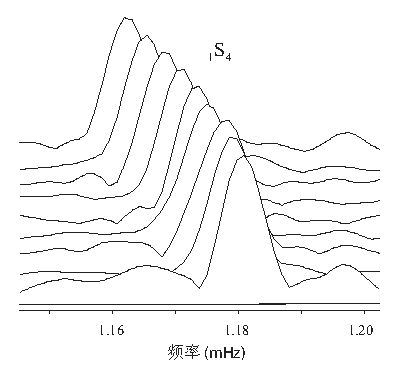
\includegraphics{../figures/chap14/fig04.eps}
\end{center}
\caption[1S4_strip]{\label{fig:14.1S4_strip}
\iffalse
Singlet strips $|\eta_m(\omega)|$ of the spheroidal overtone
${}_1{\rm S}_4$. The nine strips are displayed in order with
$|\eta_{-4}(\omega)|$ in back and $|\eta_{4}(\omega)|$ in front.
(Courtesy of G. Masters.)
\fi
%%%
球型泛音~${}_1{\rm S}_4$~的单态条带~$|\eta_m(\omega)|$。9~个剥离谱峰按顺序排列,且~$|\eta_{-4}(\omega)|$~在后,$|\eta_{4}(\omega)|$~在前。(由~G. Masters~提供)
%%%
}
\end{figure}
\iffalse
This technique---which is known as {\em singlet stripping\/}---was
\index{singlet stripping}%
developed by Buland, Berger \& Gilbert (\citeyear{buland&al79}) and
perfected and widely applied by Ritzwoller, Masters \& Gilbert
(\citeyear{ritzwoller&al86}) and \textcite{widmer91}.
The renormalization factor in~(\ref{14.Amdef}) is commonly
ignored in applications; that is, the amplitude of each
singlet in~(\ref{eq:14.strips}) is approximated by $A_m\approx
\tilde{r}_m^{*}\tilde{s}_m$.  The method presumes that the
lateral heterogeneity of the Earth is predominantly zonal;
it happens there are a number of isolated multiplets for which
this is an acceptable approximation.  The spheroidal mode
${}_1{\rm S}_4$, which is visibly split, as seen in
Figure~\ref{fig:14.lp_spec}, is an excellent example.
Figure~\ref{fig:14.1S4_strip} shows the resulting
strips $|\eta_m(\om)|$, arranged in order $-4\leq m\leq 4$
from back to front.  The nearly uniform peak spacing is an
indication that the splitting of this multiplet is
primarily a consequence of the first-order Coriolis force.
In fact, the measured singlet eigenfrequencies
$\om_0+\delta\om_m$ agree extremely well with the
theoretical peak distribution $\delta\om_m=\om_0(a+bm+cm^2)$
upon a rotating, elliptical Earth, as seen
in~Figure~\ref{fig:14.1S4}.
\fi
%%%
这种技术被称为单态模式剥离,由Buland, Berger \& Gilbert~(\citeyear{buland&al79})~提出,并由~Ritzwoller, Masters \& Gilbert~(\citeyear{ritzwoller&al86})~和~\textcite{widmer91}~完善和广泛应用。(\ref{14.Amdef})~式中的重归一化因子在应用中通常被忽略;也即,式~(\ref{eq:14.strips})~中每个单态模式的振幅可近似表示为~$A_m\approx
\tilde{r}_m^{*}\tilde{s}_m$。该方法假设地球的横向不均匀性主要是带状的;由于存在众多孤立多重态,因此该近似是可接受的。如图~\ref{fig:14.lp_spec}~所示,明显分裂的球型模式~${}_1{\rm S}_4$~是一个较好的例子。图~\ref{fig:14.1S4_strip}~显示了获得的条带$|\eta_m(\om)|$ ,且以级数$-4\leq m\leq 4$ 的顺序从后向前排列。近乎均匀的谱峰间距表明,该多重态分裂主要是一阶科里奥利力所致。事实上,如图~\ref{fig:14.1S4}~所示,在有旋椭球地球上,单态本征频率观测值~$\om_0+\delta\om_m$~与理论谱峰分布~$\delta\om_m=\om_0(a+bm+cm^2)$~极为一致。
%%%
\index{singlet stripping|)}%
\index{stripping!singlet|)}%
\begin{figure}[!t]
\begin{center}
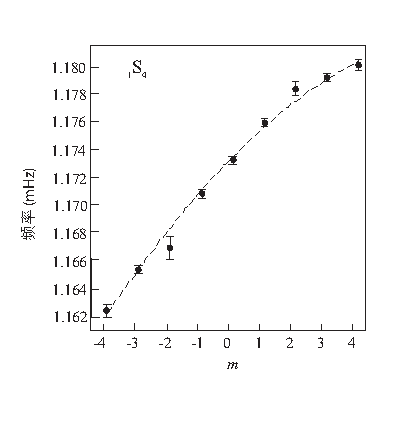
\includegraphics{../figures/chap14/fig05.eps}
\end{center}
\caption[1S4]{\label{fig:14.1S4}
\iffalse
Observed singlet eigenfrequencies $\omega_0+\delta\omega_m$
for mode ${}_1{\rm S}_4$.  These have been measured
by fitting a separate Lorentzian to each of the nine strips
in Figure~\protect\ref{fig:14.1S4_strip}. Each fit is performed
in the {\em complex\/} spectral domain,
i.e., to $\eta_m(\omega)$ rather than $|\eta_m(\omega)|$.
Error bars denote the $\pm\sigma$ uncertainty.
The predicted eigenfrequency splitting
$\delta\omega_m=\omega_0(a+bm+cm^2)$
due to the Earth's rotation and hydrostatic ellipticity
is indicated by the dashed line.
(Courtesy of G. Masters.)
\fi
%%%
模式~${}_1{\rm S}_4$~的单态本征频率观测值~$\omega_0+\delta\omega_m$。该观测结果是采用独立洛伦兹函数拟合图~\protect\ref{fig:14.1S4_strip}~中~9~个条带获取的。每次拟合都是在复谱域内进行的,即对~$\eta_m(\omega)$~进行拟合,而非$|\eta_m(\omega)|$。误差棒表示不确定度~$\pm\sigma$。虚线表示由地球自转和流体静力学平衡椭率导致的预测本征频率分裂~$\delta\omega_m=\omega_0(a+bm+cm^2)$。(由~G. Masters~提供)
%%%
}
\end{figure}

%\subsection{Anomalously split modes}
\subsection{异常分裂模式}
\index{mode!anomalous|(}%
\index{anomalous mode|(}%
\index{anomalous splitting|(}%
\index{splitting!anomalous|(}%
\label{14.sec.incsplit}

\iffalse
Figure~\ref{fig:14.18S4} shows the singlet strips
of the PKIKP-equivalent multiplet ${}_{18}{\rm S}_4$.
The observed peak distribution of this mode {\em cannot\/}
be attributed to the Earth's rotation and hydrostatic
ellipticity; the total splitting width $\Delta\om
\approx\delta\om_0-\delta\om_{\pm 4}$ is almost twice
as large as that predicted.  The success of the stripping
procedure is a clear indication that
the causative perturbation is axially symmetric;
however, very large coefficients $\sigma_{20},
\sigma_{40},\sigma_{60},\sigma_{80}$
are required if $\Delta\om$ is attributed to non-hydrostatic
zonal heterogeneity, as in equation~(\ref{14.zonal}).
Similarly strong non-hydrostatic---and apparently
zonal---splitting is a characteristic feature of
approximately twenty other {\em core-sensitive\/}
spheroidal multiplets,
\index{mode!core-sensitive}%
\index{core-sensitive mode}%
including ${}_3{\rm S}_2$,
${}_9{\rm S}_3$ and ${}_{13}{\rm S}_2$.
The mantle can be eliminated as a source, since its
decidedly non-zonal structure is well constrained by
other non-anomalously split modes, as we shall see in
the next section.
\fi
%%%
图~\ref{fig:14.18S4}~显示了~PKIKP~等效多重态~${}_{18}{\rm S}_4$~的单态条带。该模式的观测谱峰分布不能归因于地球的自转和流体静力学椭率;其总分裂宽度~$\Delta\om
\approx\delta\om_0-\delta\om_{\pm 4}$~几乎是预测值的两倍。该剥离过程的成功表明了诱发的微扰是轴对称的;但是,如果将~$\Delta\om$~归因于非流体静力学带状不均匀性,则需要如式~(\ref{14.zonal})~所示的大量系数~$\sigma_{20}$、$\sigma_{40}$、$\sigma_{60}$~和~$\sigma_{80}$。类似的强非流体静力学且明显带状的分裂是约~20~个其他核敏感球型多重态(包括~${}_3{\rm S}_2$、${}_9{\rm S}_3$~和~${}_{13}{\rm S}_2$)的特征。地幔可被排除为一个源,因为其绝对非带状结构很好地受到其他非异常分裂模式的限制,见下一节。
%%%
\begin{figure}[!t]
\begin{center}
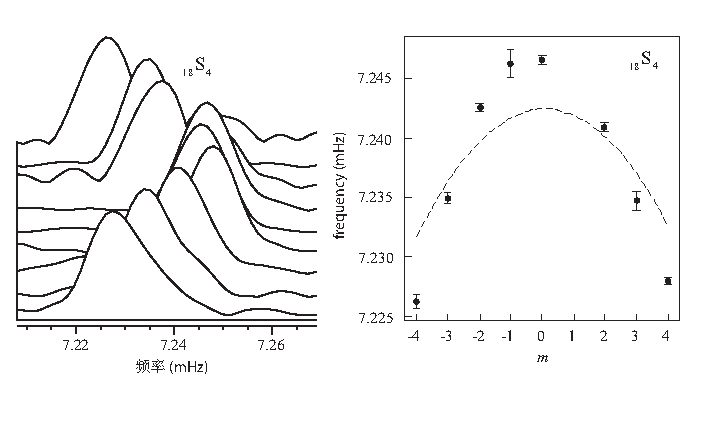
\includegraphics{../figures/chap14/fig06.eps}
\end{center}
\caption[18S4]{\label{fig:14.18S4}
\iffalse
({\em  Left}) Singlet strips $|\eta_m(\omega)|$ of the
anomalously split multiplet ${}_{18}{\rm S}_4$.
The nine strips are displayed in order with
$|\eta_{-4}(\omega)|$ in back and $|\eta_{4}(\omega)|$ in front.
({\em  Right}) The observed singlet eigenfrequencies
$\omega_0+\delta\omega_m$ exhibit a quasi-parabolic
$\delta\omega_m\approx\omega_0(a'+c'm^2)$ dependence
upon the order $m$; however, the strength of the splitting
is much greater than that due to the Earth's rotation
and hydrostatic ellipticity, indicated by the dashed line.
(Courtesy of R. Widmer.)
\fi
%%%
(左图)异常分裂多重态~${}_{18}{\rm S}_4$~的单态条带~$|\eta_m(\omega)|$。9~个条带按顺序排列,且~$|\eta_{-4}(\omega)|$~在后,$|\eta_{4}(\omega)|$~在前。(右图)单态观测本征频率~$\omega_0+\delta\omega_m$~呈现出一个依赖级数~$m$~的准抛物线型~$\delta\omega_m\approx\omega_0(a'+c'm^2)$;然而,其分裂强度要比虚线所示的地球自转和流体静力学椭率所导致的强度大得多。(由~R. Widmer~提供)
%%%
}
\end{figure}

\iffalse
The nature of this so-called {\em anomalous splitting\/}
remained a controversial enigma for more than a decade,
following its discovery by \textcite{masters&gilbert81}.
A number of possible explanations were proposed and
investigated during this period:
\fi
%%%
自~\textcite{masters&gilbert81}~发现这种所谓的异常分裂后,十多年来,它的本质一直是一个有争议的谜题。在此期间,相关学者提出并调查了若干可能的解释:
%%%
\begin{enumerate}
\item
\iffalse
Some of the anomalously split modes have less than three
percent of their compressional energy within the solid inner
core.  This led to speculation that the splitting might be
produced by degree-two heterogeneity of the compressional-wave
speed $\delta\hspace{-0.1 mm}\alpha_{20}$ within the
{\em fluid outer core\/}
(Ritzwoller, Masters \& Gilbert
\citeyear{ritzwoller&al88}; Widmer, Masters \& Gilbert 1992).
\nocite{widmer&al92}
Such a model can be tweaked to
fit the observed anomalous splitting; however, the corresponding
variations $\delta\hspace{-0.2 mm}\rho_{20}$ in fluid-core
density are ruled out by the hydrostatic considerations in
Section~\ref{13.sec.SNREI} (Stevenson \citeyear{stevenson87}).
\fi
%%%
一些异常分裂模式在固态内核中只有不到3\%的压缩能量。这引起猜测该分裂可能是由液态外核压缩波速度的二阶不均匀性~$\delta\hspace{-0.1 mm}\alpha_{20}$~造成的~(Ritzwoller, Masters \& Gilbert
\citeyear{ritzwoller&al88}; Widmer, Masters \& Gilbert 1992).
\nocite{widmer&al92}。这种模型可被调整以适应观测异常分裂;然而,采用~\ref{13.sec.SNREI}~节的流体静力学考虑,相应的液核密度变化~$\delta\hspace{-0.2 mm}\rho_{20}$~被排除~(Stevenson \citeyear{stevenson87})。
%%%
\item
\iffalse
Degree-two topographic variations
$\delta\hspace{-0.1 mm}d_{st}$ on either the
inner-core or core-mantle boundaries are also capable
of explaining the observed anomalous splitting;
however, such large non-hydrostatic boundary perturbations
are inconsistent with body-wave travel-time data
(Ritzwoller, Masters \& Gilbert \citeyear{ritzwoller&al88};
Widmer, Masters \& Gilbert 1992).
\fi
%%%
内核或核幔边界上的二阶地形变化~$\delta\hspace{-0.1 mm}d_{st}$~也能够解释观测异常分裂;然而,这种大的非流体静力学边界微扰与体波走时数据并不一致~(Ritzwoller, Masters \& Gilbert \citeyear{ritzwoller&al88};
Widmer, Masters \& Gilbert 1992)。
%%%
\item
\iffalse
\textcite{tanimoto89} showed conclusively that the Earth's magnetic
field cannot be responsible for the observed anomalous splitting.
\fi
%%%
\textcite{tanimoto89}~明确指出,地球磁场不可能是导致观测异常分裂的原因。
%%%
\item
\iffalse
\textcite{gilbert94} demonstrated that the effect of large-scale
convective flow in the fluid outer core is likewise insignificant.
\fi
%%%
\textcite{gilbert94}~论证了液态外核中大尺度对流的影响同样不显著。
%%%
\item
\iffalse
Poupinet, Pillet \& Souriau (\citeyear{poupinet&al83})
were the first to note that PKIKP waves traversing
the inner core along a ray path parallel to the
Earth's rotation axis arrive several seconds faster
than PKIKP waves travelling in the equatorial plane.
Motivated by this observation, Morelli, Dziewonski
\& Woodhouse (\citeyear{morelli&al86}) and Woodhouse,
Giardini \& Li (\citeyear{woodhouse&al86}) proposed
{\em inner-core anisotropy\/}
\index{inner-core anisotropy}%
\index{anisotropy!inner-core}%
as an explanation for both the
anomalous PKIKP travel times and the anomalous splitting
of the core-sensitive spheroidal modes.
\fi
%%%
Poupinet, Pillet \& Souriau~(\citeyear{poupinet&al83})首次注意到,沿平行于地球自转轴的射线路径穿过内核的~PKIKP~波要比沿赤道面传播快的~PKIKP~波快几秒到达。基于这一观测结果,Morelli, Dziewonski
\& Woodhouse (\citeyear{morelli&al86})~和~Woodhouse,
Giardini \& Li (\citeyear{woodhouse&al86})~提出了内核各向异性可以解释~PKIKP~波的异常走时和核敏感球型模式的异常分裂。
%%%
\item
\iffalse
More comprehensive body-wave studies subsequently confirmed
the presence of compressional-wave anisotropy of a few percent
throughout the inner core (Creager \citeyear{creager92};
Shearer \citeyear{shearer94}; Song \& Helmberger
\citeyear{song&helmberger95}).  Nevertheless, the
structure responsible for the anomalous multiplet
splitting continued to be debated.  After a thorough
analysis of more than twenty PKIKP-equivalent modes,
Widmer, Masters \& Gilbert (1992)
dismissed inner-core anisotropy as a viable explanation,
because the model of Li, Giardini \& Woodhouse (\citeyear{li&al91})
was inconsistent with their data.
\fi
%%%
更全面的体波研究随后证实了内核压缩波各向异性的存在,且只有几个百分点~(Creager \citeyear{creager92};
Shearer \citeyear{shearer94}; Song \& Helmberger
\citeyear{song&helmberger95})。然而,引起异常多重态分裂的结构仍存在争议。在深入分析了超过~20~个~PKIKP~等效模式后,Widmer, Masters \& Gilbert (1992)~排除了内核各向异性作为一种可行的解释,因为~Li, Giardini \& Woodhouse (\citeyear{li&al91})~的模型与其数据并不一致。
%%%
\end{enumerate}
\iffalse
Taking a new analytical approach, Tromp (\citeyear{tromp93})
showed that all of the anomalous multiplet measurements
are consistent with a simple transversely isotropic
inner-core model having a symmetry axis aligned with the
Earth's rotation.
As demonstrated in Appendix~D.4.4, this type of
anisotropy gives rise to a diagonal splitting matrix
$\ssH^{\rm ani}=(2\om_0)^{-1}\ssV^{\rm ani}$, with elements
\fi
%%%
采用一种新的分析方法,Tromp~(\citeyear{tromp93})~表明所有异常多重态观测结果都符合一个简单的横向各向同性内核模型,其对称轴与地球自转方向一致。如附录~D.4.4~所示,这种各向异性会产生一个对角化分裂矩阵~$\ssH^{\rm ani}=(2\om_0)^{-1}\ssV^{\rm ani}$,包含元素
%%%
\eqa \label{14.Hani}
\lefteqn{
H_{mm'}^{\rm ani}=\delta_{mm'}\,\sum_{s=0,2,4}(-1)^m
\left(\frac{2l+1}{2\om_0}\right)\left(\frac{2s+1}{4\pi}\right)^{1/2}
}
\nonumber \\
&&\mbox{}\qquad
\times\left(\begin{array}{ccc}
l & s & l  \\
-m & 0 & m
\end{array}\right)
\sum_{N}\sum_{I}\int_0^c\Gamma_{N\hspace{-0.3 mm}I}\,r^2dr.      
\ena
\begin{figure}
\begin{center}
\scalebox{0.867}{
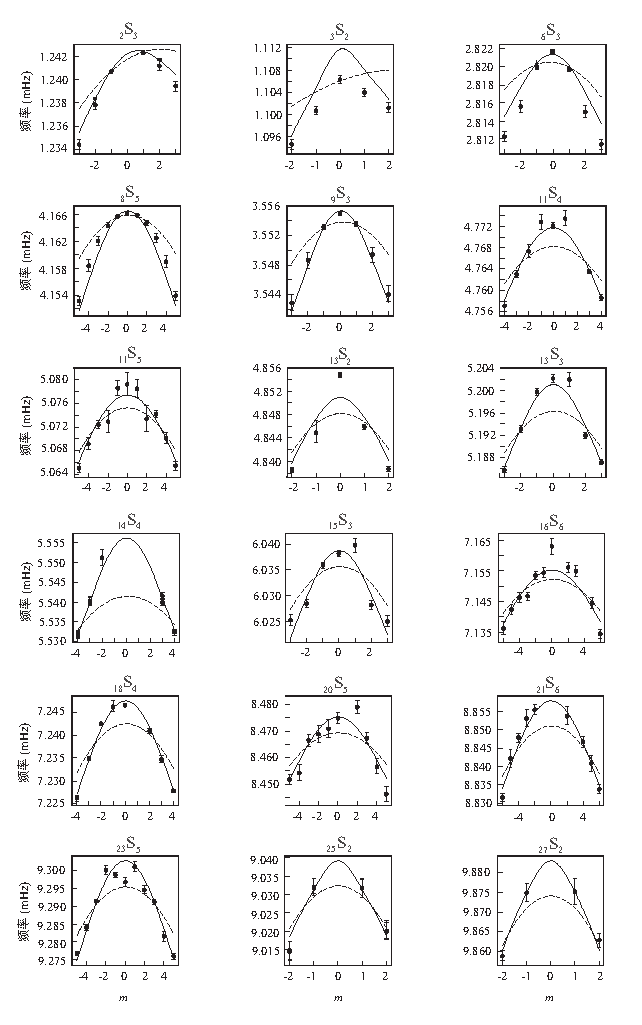
\includegraphics{../figures/chap14/fig07.eps}
}
\end{center}
\caption[anomalousmodes]{\label{fig:14.anomalousmodes}
\iffalse
Observed singlet eigenfrequencies $\omega_0+\delta\omega_m$ of
eighteen anomalously split multiplets (courtesy of R. Widmer).
The splitting of all of these modes is larger than that due to
the Earth's rotation and hydrostatic ellipticity ({\em dashed line\/}).
The combined effects $\delta\omega_m=\omega_0(a+bm+cm^2)+\omega_0
(a'+c'm^2+dm^4)$ of rotation, ellipticity and co-axial inner-core
anisotropy ({\em solid line\/}) provide a much more
satisfactory fit to the data.
\fi
%%%
18~个异常分裂多重态的观测单态本征频率~$\omega_0+\delta\omega_m$(由~R. Widmer~提供)。所有这些模式的分裂宽度都大于地球自转和流体静力学椭率所导致的结果(虚线)。地球自转、椭率和同轴内核各向异性(实线)的联合效应~$\delta\omega_m=\omega_0(a+bm+cm^2)+\omega_0
(a'+c'm^2+dm^4)$~可提供与实测数据更吻合的拟合结果。
%%%
}
\end{figure}
\iffalse
The non-zero kernels $\Gamma_{01}$--$\Gamma_{05}$,
$\Gamma_{11}$--$\Gamma_{13}$,
$\Gamma_{21}$--$\Gamma_{23}$, $\Gamma_{31}$ and $\Gamma_{43}$ are
defined in equations~(\ref{D.208})--(\ref{D.220}).
The combined effects of rotation, ellipticity
and co-axial inner-core anisotropy are
governed by
\fi
%%%
其中,非零核函数~$\Gamma_{01}$--$\Gamma_{05}$、$\Gamma_{11}$--$\Gamma_{13}$、$\Gamma_{21}$--$\Gamma_{23}$、$\Gamma_{31}$~和~$\Gamma_{43}$~在式~(\ref{D.208})--(\ref{D.220})~中被定义。地球自转、椭率和同轴内核各向异性的综合效应可由如下公式控制
%%%
\eq \label{14.JeroenH}
\ssH^{\rm rot+ell+ani}=\ssW+(2\om_0)^{-1}
(\ssV^{\rm ell+cen}+\ssV^{\rm ani}-\om_0^2\ssT^{\rm ell}).
\en
\iffalse
The order $m$ of the complex spherical harmonic $Y_{lm}$
remains a good quantum number; the resulting eigenfrequency
perturbations can be reduced with the aid
of~(\ref{C.needinD1})--(\ref{C.needinD2})
to a compact form:
\fi
%%%
复球谐函数~$Y_{lm}$~的级数~$m$~仍然是一个好量子数;利用~(\ref{C.needinD1})--(\ref{C.needinD2})~式可将所得到的本征频率微扰简化为一个简洁形式:
%%%
\eq \label{14.acd}
\delta\om_m=\om_0(a+bm+cm^2)+\om_0(a'+c'm^2+dm^4),
\en
\iffalse
where the first term accounts for the rotation and ellipticity
and the second accounts for the anisotropy.
The additional constant, quadratic and quartic splitting coefficients
$a'$, $c'$, and $d$ are given by
\fi
%%%
其中,第一项解释了自转和椭率,第二项解释了各向异性。附加常数、二次和四次分裂系数~$a'$、$c'$~和~$d$~可表示为
%%%
\eqa
a'\hspace{-2 mm}&=&\hspace{-2 mm}\half\om_0^{-2}(-1)^l(2l+1)\biggl\{
\left[\frac{(2l)!}{(2l+1)!}\right]^{1/2}K_0 \nonumber \\
&&\mbox{}-2l(l+1)\left[\frac{(2l-2)!}{(2l+3)!}\right]^{1/2}K_2 \nonumber \\
&&\mbox{}+6(l+2)(l+1)l(l-1)\left[
\frac{(2l-4)!}{(2l+5)!}\right]^{1/2}K_4\biggr\}, \label{14.aaniso} \\
c'\hspace{-2 mm}&=&\hspace{-2 mm}\half\om_0^{-2}(-1)^l(2l+1)\biggl\{
6\left[\frac{(2l-2)!}{(2l+3)!}\right]^{1/2}K_2 \nonumber \\
&&\mbox{}+[50-60l(l+1)]\left[\frac{(2l-4)!}{(2l+5)!}\right]^{1/2}K_4\biggr\}, \\
d\hspace{-2 mm}&=&\hspace{-2 mm}\half\om_0^{-2}(-1)^l(2l+1)\biggl\{
70\left[\frac{(2l-4)!}{(2l+5)!}\right]^{1/2}K_4\biggr\}, \label{14.daniso}
\ena
\iffalse
where
\fi
%%%
其中,
%%%
\eq
K_s=\sum_N\sum_I\left(\frac{2s+1}{4\pi}\right)^{1/2}
\int_0^c\Gamma_{N\hspace{-0.3 mm}I}\,r^2dr,\qquad s=0,2,4.
\en
\iffalse
The observed eigenfrequency perturbations $\delta\om_m$,
$-l\leq m\leq l$,
of the anomalously split multiplets may be used to constrain the radial
distribution of the five transversely isotropic perturbations
$\delta C$, $\delta\hspace{-0.3 mm}A$, $\delta\hspace{-0.3 mm}L$,
$\delta\hspace{-0.3 mm}N$, $\delta\hspace{-0.3 mm}F$ within the
inner core.  Figure~\ref{fig:14.anomalousmodes} shows the fit of
such a transversely isotropic inner-core model to the splitting
of eighteen well-characterized core-sensitive spheroidal modes
(Tromp \citeyear{tromp93}).
\fi
%%%
异常分裂多重态的观测本征频率微扰~$\delta\om_m$($-l\leq m\leq l$)可用来约束五个横向各向同性微扰~$\delta C$、$\delta\hspace{-0.3 mm}A$、$\delta\hspace{-0.3 mm}L$、$\delta\hspace{-0.3 mm}N$~和~$\delta\hspace{-0.3 mm}F$~在内核中的径向分布。图~\ref{fig:14.anomalousmodes}~展示了这一横向各向同性内核模型与~18~个表征良好的核敏感球型模式分裂的符合情况~(Tromp \citeyear{tromp93})。
%%%
\index{mode!anomalous|)}%
\index{anomalous mode|)}%
\index{anomalous splitting|)}%
\index{splitting!anomalous|)}%

%\subsection{Splitting function}
\subsection{分裂函数}
\index{splitting function|(}%
\index{spectral fitting|(}%
\label{14.sec.splitfcn}

\iffalse
Singlet stripping is based upon the presumption that
the order $m$ of a complex spherical harmonic $Y_{lm}$
is a good quantum number; for this reason, it cannot
be implemented whenever the predominant perturbation
affecting an isolated multiplet is non-zonal.  Instead,
we must deal with the non-sparse $(2l+1)\times(2l+1)$
splitting matrix~(\ref{14.HSELF})--(\ref{14.H_self}).
Giardini, Li \& Woodhouse (\citeyear{giardini&al87};
\citeyear{giardini&al88}) and Ritzwoller, Masters
\& Gilbert (\citeyear{ritzwoller&al86};
\citeyear{ritzwoller&al88}) developed an innovative two-step
{\em spectral fitting\/} procedure which may be applied
in this more general case.  The method ignores lateral
variations in anelasticity and eigenfunction
renormalization; with those provisos, the spectral
response~(\ref{eq:14.aom}) of an isolated
multiplet can be written in terms of the original
receiver and source vectors $\ssr$ and $\sss$ in
the form
\fi
%%%
单态模式剥离是基于复球谐函数~$Y_{lm}$~的级数~$m$~是一个好量子数的假设;鉴于这一原因,当影响孤立多重态的主要微扰是非带状时,这种假设是不成立的。相反地,我们必须处理非稀疏的~$(2l+1)\times(2l+1)$~维分裂矩阵~(\ref{14.HSELF})--(\ref{14.H_self})。Giardini, Li \& Woodhouse~(\citeyear{giardini&al87};
\citeyear{giardini&al88})~和~Ritzwoller, Masters \& Gilbert~(\citeyear{ritzwoller&al86};
\citeyear{ritzwoller&al88})~提出了一种创新的两步频谱拟合方法,可应用于这种更一般的情况。该方法忽略了非弹性的横向变化和本征函数的重归一化;在这些条件下,孤立多重态的频谱响应~(\ref{eq:14.aom})~式可用原始接收点向量~$\ssr$~和震源向量~$\sss$~来表示
%%%
\eq \label{14.myaom}
a(\omega)=\half i\hspace{0.1 mm}\ssr^{\rm T}
[\ssH-(\omega-\omega_0-i\gamma_0)\ssI]^{-1}\sss,
\en
\iffalse
where $\ssH=\ssW+(2\om_0)^{-1}[\ssV^{\rm ell+cen}+
\ssV^{\rm lat}-\om_0^2(\ssT^{\rm ell}+\ssT^{\rm lat})]$.
Each spectrum~(\ref{14.myaom}) depends upon the 
source $\bM$, $\bx_{\rm s}$, the receiver $\bnuh$,
$\bx$, the rotational and elliptical splitting
coefficients $a$, $b$, $c$, and the elastic-structure
coefficients $\sigma_{st}$, $s=2,4,\ldots,2l$,
$t=-s,\ldots,0,\ldots,s$.  Assuming that the source and
receiver parameters and the rotation and ellipticity
of the Earth are known, it is possible to solve for
the $5+9+\cdots +(4l+1)=l(2l+3)$ unknown coefficients $\sigma_{st}$
by minimizing the misfit between a suite of observed and
synthetic spectra $a_p(\om),\,p=1,2,\ldots$, in an iterative, non-linear
least-squares inversion.  Perturbation of~(\ref{14.myaom})
yields the derivatives $\p a_p/\p\sigma_{st}$ needed
to converge upon the minimum:
\fi
%%%
其中,$\ssH=\ssW+(2\om_0)^{-1}[\ssV^{\rm ell+cen}+
\ssV^{\rm lat}-\om_0^2(\ssT^{\rm ell}+\ssT^{\rm lat})]$。每个频谱~(\ref{14.myaom})~式取决于震源~$\bM$~和~$\bx_{\rm s}$、接收点~$\bnuh$~和~$\bx$、自转和椭率分裂参数~$a$、$b$、$c$~以及弹性结构系数~$\sigma_{st}$, $s=2,4,\ldots,2l$,
$t=-s,\ldots,0,\ldots,s$。假设震源和接收点参数以及地球的自转和椭率已知,在迭代、非线性最小二乘反演中,通过使一组观测谱和合成谱~$a_p(\om),\,p=1,2,\ldots$~差值最小,就有可能解出~$5+9+\cdots +(4l+1)=l(2l+3)$~个未知系数~$\sigma_{st}$。式~(\ref{14.myaom})~的微扰产生的导数~$\p a_p/\p\sigma_{st}$~需收敛于如下最小值:
%%%
\eqa \label{14.Frechet} \lefteqn{
\delta a(\om)=-\half i\hspace{0.1 mm}\ssr^{\rm T}
[\ssH-(\omega-\omega_0-i\gamma_0)\ssI]^{-1}} \nonumber \\
&&\mbox{}\qquad\qquad\times\ssdelta\ssH
\hspace{0.4 mm}[\ssH
-(\omega-\omega_0-i\gamma_0)\ssI]^{-1}\sss,
\ena
\iffalse
where we have ignored the renormalization terms in
equation~(\ref{13.born7}).  Note that it is possible
to combine spectra $a_p(\om)$ from many different
earthquakes $\bM$, $\bx_{\rm s}$ as well as receivers
$\bnuh$, $\bx$.  Since the
number of potentially available spectra is much
larger than $l(2l+3)$, it is possible to
obtain a strong constraint upon the coefficients
$\sigma_{st}$ characterizing a multiplet.  This
first step in the procedure is repeated for as many
isolated modes as can be identified in the spectra.
The quality of the spectral fits that can be obtained is
illustrated in Figure~\ref{fig:14.inifin}.
In the second step, the splitting coefficients
of all of the analyzed modes are simultaneously
inverted to find the even-degree lateral variations
in incompressibility, rigidity, density
and boundary topography.  Equation~(\ref{eq:14.cst})
describes the strictly linear dependence of $\sigma_{st}$
upon the perturbations $\delta\hspace{-0.1 mm}\kappa_{st}$,
$\delta\hspace{-0.2 mm}\mu_{st}$, $\delta\hspace{-0.2 mm}\rho_{st}$
and $\delta\hspace{-0.1 mm}d_{st}$.  The spectral-fitting method
has been refined and applied by a number of investigators,
including Li, Giardini \& Woodhouse (\citeyear{li&al91}; \citeyear{li&al91b}),
Widmer, Masters \& Gilbert (1992),\nocite{widmer&al92}
He \& Tromp (\citeyear{he&tromp96}) and Resovsky \& Ritzwoller
(\citeyear{resovsky&ritzwoller98});
a comprehensive summary and comparison of results obtained prior
to the occurrence of the June 9, 1994, Bolivia earthquake is
given by Ritzwoller \& Lavely (\citeyear{ritzwoller&lavely95}).
\fi
%%%
此处,我们忽略了式~(\ref{13.born7})~中的重归一化项。注意,此时可以联合众多不同地震~$\bM$、$\bx_{\rm s}$~和接受点~$\bnuh$、$\bx$~的频谱~$a_p(\om)$。由于潜在可用谱的数量远远大于~$l(2l+3)$,因此有可能得到描述某一多重态的系数~$\sigma_{st}$~的强约束。在频谱中识别尽可能多的孤立模式以重复该过程的第一步。图~\ref{fig:14.inifin}~展示了可获取的频谱拟合结果。第二步,同时反演所有分析模式的分裂系数,以求得不可压缩性、刚性、密度和边界地形的偶数阶横向变化。式~(\ref{eq:14.cst})~描述了~$\sigma_{st}$~对~$\delta\hspace{-0.1 mm}\kappa_{st}$、$\delta\hspace{-0.2 mm}\mu_{st}$、$\delta\hspace{-0.2 mm}\rho_{st}$~和~$\delta\hspace{-0.1 mm}d_{st}$~的严格线性依赖性。频谱拟合方法已被众多学者改进和应用,包括~Li, Gi ardini \& Woodhouse~(\citeyear{li&al91}; \citeyear{li&al91b})、Widmer, Masters \& Gilbert (1992)、He \& Tromp~(\citeyear{he&tromp96})~和~Resovsky \& Ritzwoller (\citeyear{resovsky&ritzwoller98});Ritzwoller \& Lavely~(\citeyear{ritzwoller&lavely95})~对~1994~年~6~月~9~日玻利维亚地震发生前得到的结果进行了全面的总结和比较。
%%%

\iffalse
The splitting of an isolated multiplet may be conveniently
visualized in terms of its geographical {\em splitting function\/},
defined by
\fi
%%%
孤立多重态的分裂可以采用其地理分裂函数来形象化表示,即
%%%
\eq
\sigma=\sum_{\textstyle{{s=2}\atop{s\,\rm even}}}^{2l}
\sum_{t=-s}^s\sigma_{st}\sY_{st}.
\label{eq:14.splittingfunction}
\en
\iffalse
At any location $\theta,\phi$ on the Earth's surface,
the function $\sigma(\theta,\phi)$ represents a local
radial average of the underlying interior structure.
The manner in which a given mode averages
the parameters $\kappa$, $\mu$, $\rho$ and $d$
is determined by the radial kernels
$V_\kappa$, $V_\mu$, $V_\rho-\om_0^2T_\rho$
and $V_d-\om_0^2T_d$ in equation~(\ref{eq:14.cst}).
A plot of $\sigma$ can be regarded
as a representation of the geographical dependence
of the Earth's three-dimensional elastic structure,
as ``seen'' through these kernels.
The selection rules~(\ref{14.selrule}) limit the
sensitivity to even angular degrees $2\leq s\leq 2l$.
Mode ${}_8{\rm S}_1$, for example, is only sensitive to degree
two, whereas mode ${}_0{\rm S}_6$ is sensitive
to even-degree structure up to degree twelve.
Figures~\ref{fig:14.0Ssplittingfunction}
and~\ref{fig:14.0Tsplittingfunction} show the
observed splitting functions $\sigma^{\rm obs}$ for a number of
isolated fundamental-mode multiplets ${}_0{\rm S}_l$
and ${}_0{\rm T}_l$.  The coherent, predominantly $\sY_{2\,\pm 2}$
pattern is one of the most characteristic features of the Earth's
large-scale lateral heterogeneity---the shear-wave
speed is faster than average ($\delta\hspace{-0.2 mm}\beta>0$)
beneath the Americas and the Western Pacific and slower
than average ($\delta\hspace{-0.2 mm}\beta<0$) beneath the
Central Pacific and Africa.  The four kernels
$V_\kappa$, $V_\mu$, $V_\rho-\om_0^2T_\rho$
and $V_d-\om_0^2T_d$ vary smoothly along
a given mode branch, and so therefore do
the splitting functions $\sigma$.
\fi
%%%
在地表任意位置~$\theta,\phi$,函数~$\sigma(\theta,\phi)$~表示深内部结构的局地径向平均值。\textcolor{red}{为利用给定模式平均参数~$\kappa$、$\mu$、$\rho$~和~$d$,可采用式~~(\ref{eq:14.cst})~中的径向核函数~$V_\kappa$、$V_\mu$、$V_\rho-\om_0^2T_\rho$~和~$V_d-\om_0^2T_d$~确定}。通过这些核函数可以“看到”,$\sigma$~可被看作是地球三维弹性结构的地理依赖性表现。选择法则~(\ref{14.selrule})~限制其只敏感于偶数角阶数~$2\leq s\leq 2l$。例如,${}_8{\rm S}_1$~模式仅对二阶结构敏感,而~${}_0{\rm S}_6$~模式对~12~阶及以下的偶数阶结构敏感。图~\ref{fig:14.0Ssplittingfunction}~和~\ref{fig:14.0Tsplittingfunction}~显示了若干孤立基阶多重态~${}_0{\rm S}_l$~或~${}_0{\rm T}_l$~的观测分裂函数~$\sigma^{\rm obs}$。以~$\sY_{2\,\pm 2}$~为主的相干模式是地球大尺度横向不均匀性的最典型特征之一,即剪切波速比美洲和西太平洋区域下的平均值($\delta\hspace{-0.2 mm}\beta>0$)更快,比中太平洋和非洲区域下的平均值($\delta\hspace{-0.2 mm}\beta<0$)更慢。四个核函数~$V_\kappa$、$V_\mu$、$V_\rho-\om_0^2T_\rho$~和~$V_d-\om_0^2T_d$~沿一个给定的模式分支平滑变化,由此构建分裂函数~$\sigma$。
%%%

\iffalse
In principle, it is possible to allow for lateral
variations in anelasticity in the spectral-fitting
analysis by introducing a second splitting function
\fi
%%%
原则上,在频谱拟合分析中,可通过引入第二个分裂函数来考虑非弹性的横向变化,即
%%%
\eq
\psi=\sum_{\textstyle{{s=2}\atop{s\,\rm even}}}^{2l}
\sum_{t=-s}^s\psi_{st}\sY_{st}.
\label{14.splitfcn2}
\en
\iffalse
The measured coefficients $\psi_{st}$ could be
used to constrain $q_{{\kappa}st}$ and $q_{{\mu}st}$,
utilizing\hfill equation~(\ref{eq:14.ast}).\hfill  At\hfill the\hfill expense\hfill
of\hfill adding\hfill two\hfill unknowns,
it is
\fi
\begin{figure}[!t]
\begin{center}
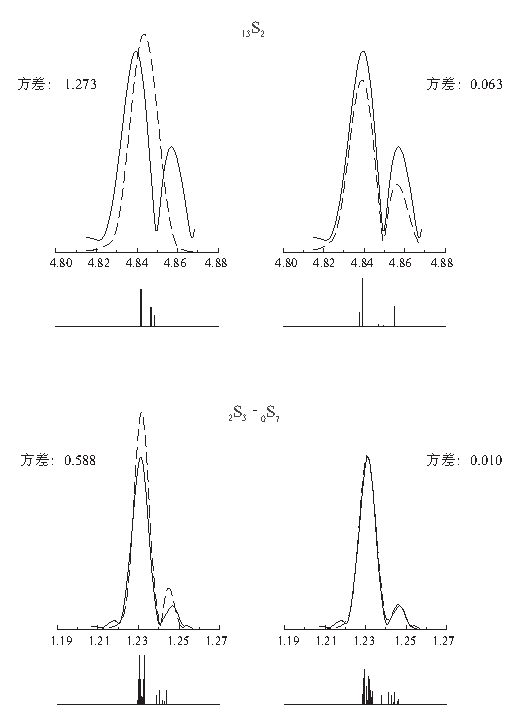
\includegraphics{../figures/chap14/fig08.eps}
\end{center}
\caption[inifin]{\label{fig:14.inifin}
\iffalse
Two examples illustrating the first step of the
spectral-fitting procedure. ({\em Top\/}) Amplitude
spectra $|a(\omega)|$ of the multiplet ${}_{13}{\rm S}_2$
recorded at station ATD in Djibouti following the
June 9, 1994 deep-focus Bolivia earthquake.
({\em Bottom\/}) Spectra of the
doublet ${}_2{\rm S}_3\!-\!{}_0{\rm S}_7$ at
station MAJO in Matsushiro, Japan following
the October 4, 1994 Kuril Islands earthquake.
Solid lines depict the observed radial-component
spectra in both cases.  Dashed lines on the left
show the initial fit of a synthetic spectrum 
which incorporates only the effects of the Earth's
rotation and hydrostatic ellipticity.  Dashed lines
on the right show the final synthetic spectrum
after fitting for the
expansion coefficients $\sigma_{st}$.  The quality of each fit is
indicated (var\hspace{0.6 mm}=\hspace{0.6 mm}
squared misfit/squared data).
Underlying line spectra show the split singlet eigenfrequencies
$\omega_0+\delta\omega_m$ or $\omega_0+\delta\omega_j$
and excitation amplitudes $|A_m|$ or $|A_j|$.
\fi
%%%
频谱拟合过程第一步的两个示例。(上图)1994~年~6~月~9~日玻利维亚深源地震后,吉布提~ATD~台站记录的多重态~${}_{13}{\rm S}_2$~的振幅谱~$|a(\omega)|$。(下图)1994~年~10~月~4~日千岛群岛地震后,日本松代~MAJO~台站的~${}_2{\rm S}_3\!-\!{}_0{\rm S}_7$~模式对的频谱。在这两个案例中,实线均描述了径向分量观测谱。左图虚线显示了只考虑地球自转和流体静力学椭率影响的合成谱初始拟合结果。右图虚线表示对膨胀系数~$\sigma_{st}$~进行拟合后的最终合成谱。每个拟合量(var\hspace{0.6 mm}=\hspace{0.6 mm}~平方偏差/平方数据)均被展示在图中。底部线谱显示了分裂单态本征频率~$\omega_0+\delta\omega_m$~或~$\omega_0+\delta\omega_j$~以及激发振幅~$|A_m|$~或~$|A_j|$。
%%%
}
\end{figure}
\begin{figure}[!t]
\begin{center}
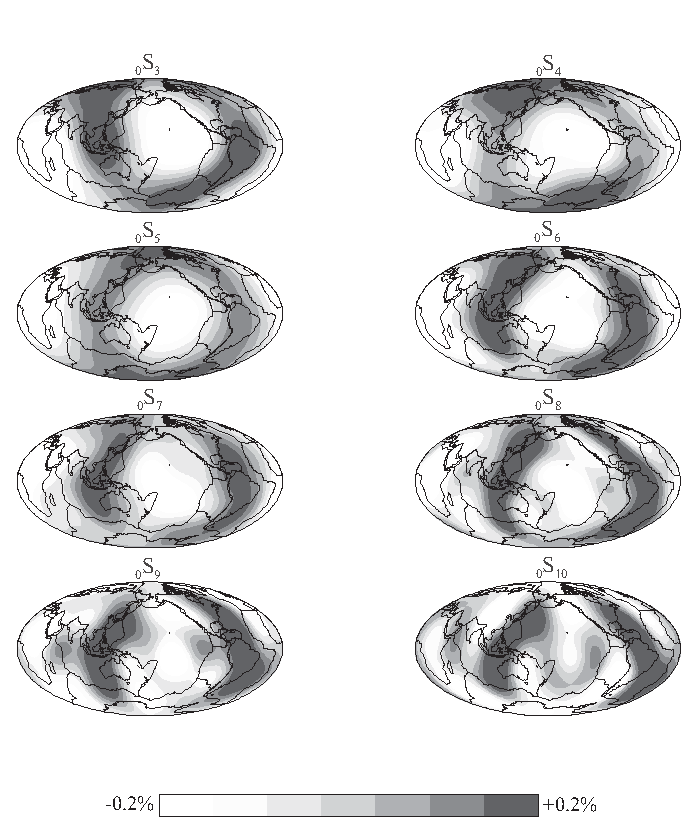
\includegraphics{../figures/chap14/fig09.eps}
\end{center}
\caption[0Ssplittingfunction]{\label{fig:14.0Ssplittingfunction}
\iffalse
Observed splitting functions $\sigma^{\rm obs}$ of the
fundamental spheroidal modes ${}_0{\rm S}_3\!-\!{}_0{\rm S}_{10}$.
Map projection is Aitoff equal-area; coastlines and tectonic plate boundaries
have been superimposed for reference.  The dark-shaded circum-Pacific
ring, where $\sigma>0$, is produced by faster-than-average shear-wave
speeds, $\delta\hspace{-0.2 mm}\beta>0$, within the underlying mantle.
The splitting functions have been truncated during the fitting,
so that each is represented by only the three lowest even degrees $s=2,4,6$.
\fi
%%%
基阶球型模式~${}_0{\rm S}_3\!-\!{}_0{\rm S}_{10}$~的观测分裂函数~$\sigma^{\rm obs}$。地图投影采用埃托夫等面积法;海岸线和构造板块边界被绘制于图中以供参考。环太平洋处的暗影($\sigma>0$)是由地幔底层中快于平均值的剪切波速度($\delta\hspace{-0.2 mm}\beta>0$)产生的。在拟合过程中,分裂函数已被截断,因此每个函数仅由三个最低偶数阶~$s=2,4,6$~表示。
%%%
}
\end{figure}
\clearpage
\begin{figure}[!t]
\begin{center}
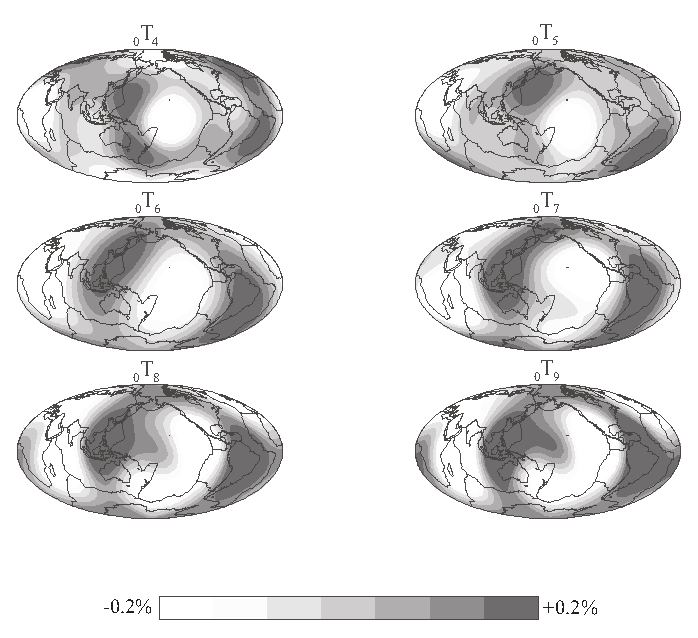
\includegraphics{../figures/chap14/fig10.eps}
\end{center}
\caption[0Tsplittingfunction]{\label{fig:14.0Tsplittingfunction}
\iffalse
Observed splitting functions $\sigma^{\rm obs}$ of the
fundamental toroidal modes ${}_0{\rm T}_4\!-\!{}_0{\rm T}_{9}$.
Map projection is Aitoff equal-area; coastlines and tectonic plate
boundaries have been superimposed for reference.
The characteristic circum-Pacific ${\cal Y}_{2\,\pm 2}$ pattern is
very similar to that exhibited by the fundamental spheroidal
modes (see Figure~\protect\ref{fig:14.0Ssplittingfunction}).
The splitting functions have been truncated during the fitting,
so that each is represented by only the three lowest even degrees $s=2,4,6$.
\fi
%%%
基阶环型模式~${}_0{\rm T}_4\!-\!{}_0{\rm T}_{9}$~的观测分裂函数~$\sigma^{\rm obs}$。地图投影采用埃托夫等面积法;海岸线和构造板块边界被绘制于图中以供参考。典型的环太平洋~${\cal Y}_{2\,\pm 2}$~模式与基阶球型模式非常相似(见图~\protect\ref{fig:14.0Ssplittingfunction})。在拟合过程中,分裂函数已被截断,因此每个函数仅由三个最低偶数阶~$s=2,4,6$~表示。
%%%
}
\end{figure}
\noindent
\iffalse
also possible to allow for degree-zero perturbations
$\delta\hspace{-0.1 mm}\kappa_{00}$, $\delta\hspace{-0.2 mm}\mu_{00}$,
\enlargethispage{-0.5\baselineskip}
$\delta\hspace{-0.2 mm}\rho_{00}$, $\delta\hspace{-0.1 mm}d_{00}$
and $q_{\kappa st}$ and $q_{\mu st}$.  The measured coefficients
$\sigma_{00}$ and $\psi_{00}$ can be used to refine the degenerate
eigenfrequency $\om^{\rm mon}_0$ and decay rate $\gamma^{\rm mon}_0$:
\fi
%%%
利用式~(\ref{eq:14.ast}),观测系数~$\psi_{st}$~可用来约束~$q_{{\kappa}st}$~和~$q_{{\mu}st}$。以增加两个未知参数为代价,也可用于约束零阶微扰~$\delta\hspace{-0.1 mm}\kappa_{00}$、$\delta\hspace{-0.2 mm}\mu_{00}$、\enlargethispage{-0.5\baselineskip}
$\delta\hspace{-0.2 mm}\rho_{00}$、$\delta\hspace{-0.1 mm}d_{00}$~和~$q_{\kappa st}$、$q_{\mu st}$。观测系数~$\sigma_{00}$~和~$\psi_{00}$~可用于简化简并本征频率~$\om^{\rm mon}_0$~和衰减率~$\gamma^{\rm mon}_0$:
%%%
\eq
\om^{\rm mon}=\om_0\left(1+\sqrt{4\pi}\,\sigma_{00}\right),
\qquad
\gamma^{\rm mon}=\gamma_0\left(1+\sqrt{4\pi}\,\psi_{00}\right).
\en
\iffalse
The resulting estimates can be used in conjunction with
other global seismological data to invert for a new terrestrial monopole.
\fi
%%%
由此得到的估计值可与其他全球地震数据联合反演一个新的地球单极子。
%%%
\begin{figure}
\begin{center}
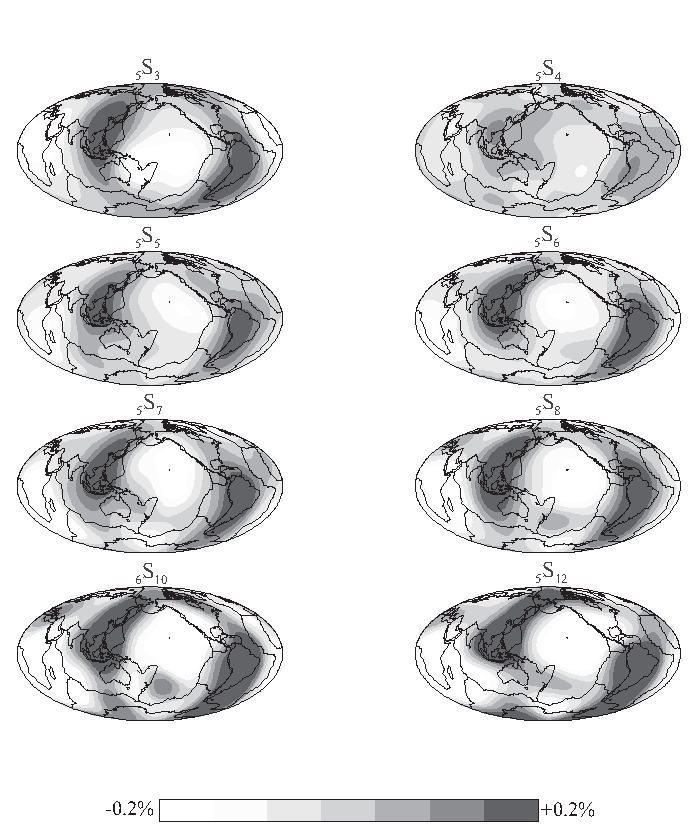
\includegraphics{../figures/chap14/fig11.eps}
\end{center}
\caption[5Ssplittingfunction]{\label{fig:14.5Ssplittingfunction}
\iffalse
Observed splitting functions $\sigma^{\rm obs}$ of selected
fifth-overtone spheroidal modes ${}_5{\rm S}_3\!-\!{}_5{\rm S}_{12}$.
Mode ${}_6{\rm S}_{10}$ has been plotted instead of ${}_5{\rm S}_{10}$
because the latter is an unobservable ${\rm J}_{\rm SV}$ inner-core mode.
Map projection is Aitoff equal-area; coastlines and tectonic plate
boundaries have been superimposed for reference.  Each of these
mantle-sensitive overtones has a predominantly ${\cal Y}_{2\,\pm 2}$
splitting function, similar to those of the fundamental modes.
Compare with the predicted splitting functions $\sigma^{\rm pre}$
of model SKS12WM13 in Figure~\protect\ref{fig:14.5Ssplittingfunction_pred}.
\fi
%%%
五阶泛音球型模式~${}_5{\rm S}_3\!-\!{}_5{\rm S}_{12}$~的观测分裂函数~$\sigma^{\rm obs}$。由于~${}_5{\rm S}_{10}$~是一个难以观测的~${\rm J}_{\rm SV}$~内核模式,因此采用~${}_6{\rm S}_{10}$~替代。地图投影采用埃托夫等面积法;海岸线和构造板块边界被绘制于图中以供参考。每个地幔敏感泛音都有一个主要的~${\cal Y}_{2\,\pm 2}$~分裂函数,类似于基阶模式。对比于图~\protect\ref{fig:14.5Ssplittingfunction_pred}~中~SKS12WM13~模型的预测分裂函数~$\sigma^{\rm pre}$。
%%%
}
\end{figure}
\begin{figure}
\begin{center}
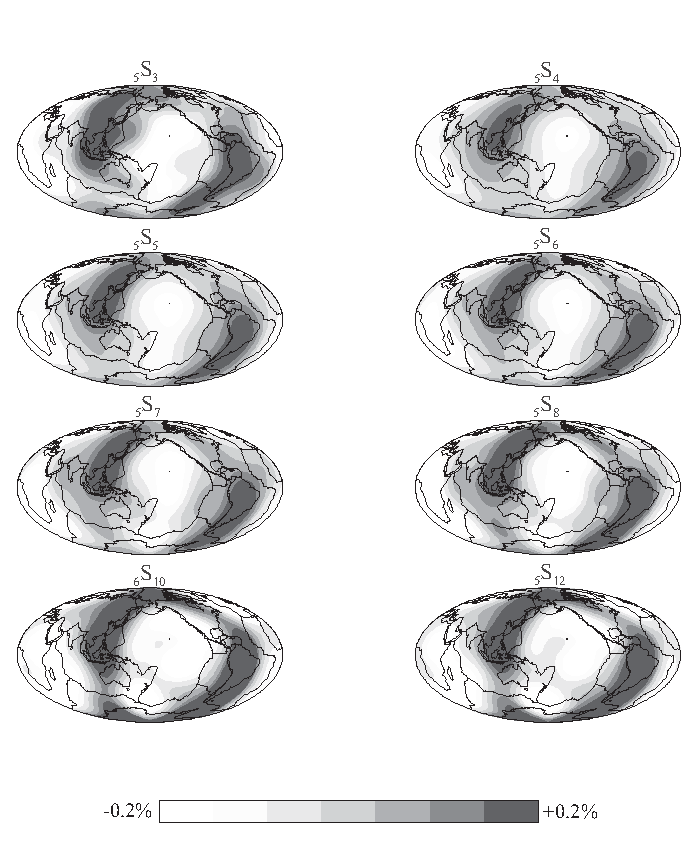
\includegraphics{../figures/chap14/fig12.eps}
\end{center}
\caption[5Ssplittingfunction_pred]{\label{fig:14.5Ssplittingfunction_pred}
\iffalse
Predicted splitting functions $\sigma^{\rm pre}$ of the eight
fifth-overtone modes in
Figure~\protect\ref{fig:14.5Ssplittingfunction}.  Model SKS12WM13
of Dziewonski, Liu \& Su (\citeyear{liu&dziewonski96}) was employed in
equations~(\ref{eq:14.cst}) and~(\ref{eq:14.splittingfunction})
to perform the calculations. Both the observed
and predicted splitting functions have been been truncated,
with only the three lowest even degrees $s=2,4,6$ retained.
\fi
%%%
图~\protect\ref{fig:14.5Ssplittingfunction}~中~8~个五阶泛音模式的预测分裂函数~$\sigma^{\rm pre}$。在式~(\ref{eq:14.cst})~和~(\ref{eq:14.splittingfunction})~中采用~Dziewonski, Liu \& Su (\citeyear{liu&dziewonski96})~的~SKS12WM13~模型进行计算。观测和预测分裂函数均已被截断,只保留三个最低偶数阶~$s=2,4,6$。
%%%
}
\end{figure}
\begin{figure}
\begin{center}
\scalebox{0.87}{
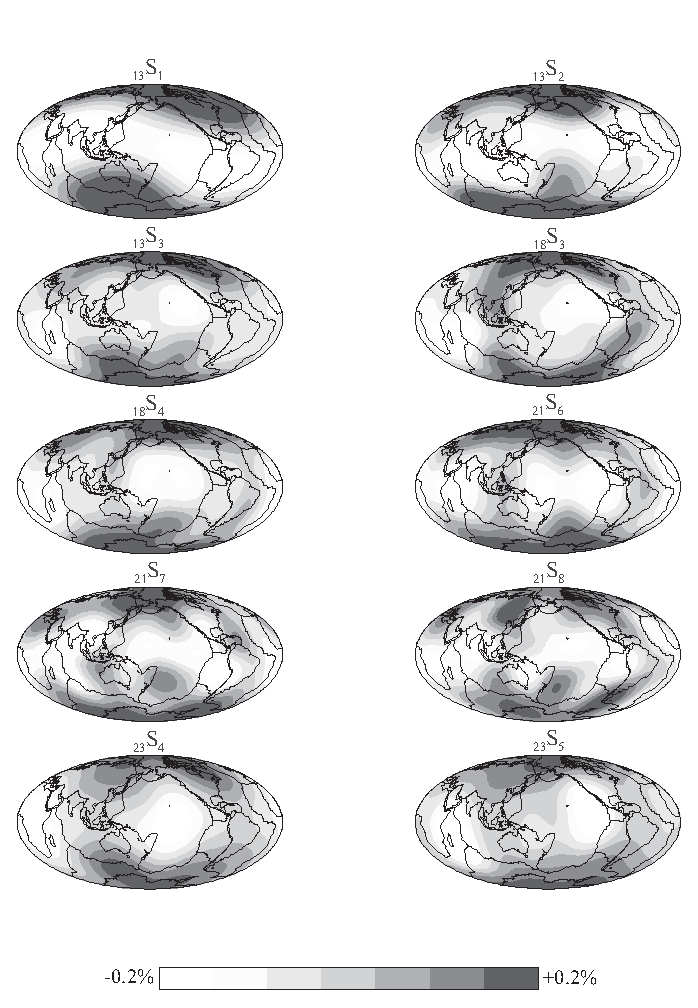
\includegraphics{../figures/chap14/fig13.eps}
}
\end{center}
\caption[core_splittingfunction]{\label{fig:14.core_splittingfunction}
\iffalse
Core-sensitive spheroidal modes such as these
exhibit an axially symmetric splitting function
that is ``fast'' ($\sigma^{\rm obs}>0$) in the vicinity of the
poles and ``slow'' ($\sigma^{\rm obs}<0$) in the vicinity of the
equator.  Map projection is Aitoff equal-area; coastlines and
tectonic plate boundaries have been superimposed for reference.
\fi
%%%
如图所示的核敏感球型模式表现为轴对称的分裂函数,且在两极附近是“快的”($\sigma^{\rm obs}>0$),在赤道附近是“慢的”($\sigma^{\rm obs}<0$)。地图投影采用埃托夫等面积法;海岸线和构造板块边界被绘制于图中以供参考。
%%%
}
\end{figure}
\begin{figure}
\begin{center}
\scalebox{0.87}{
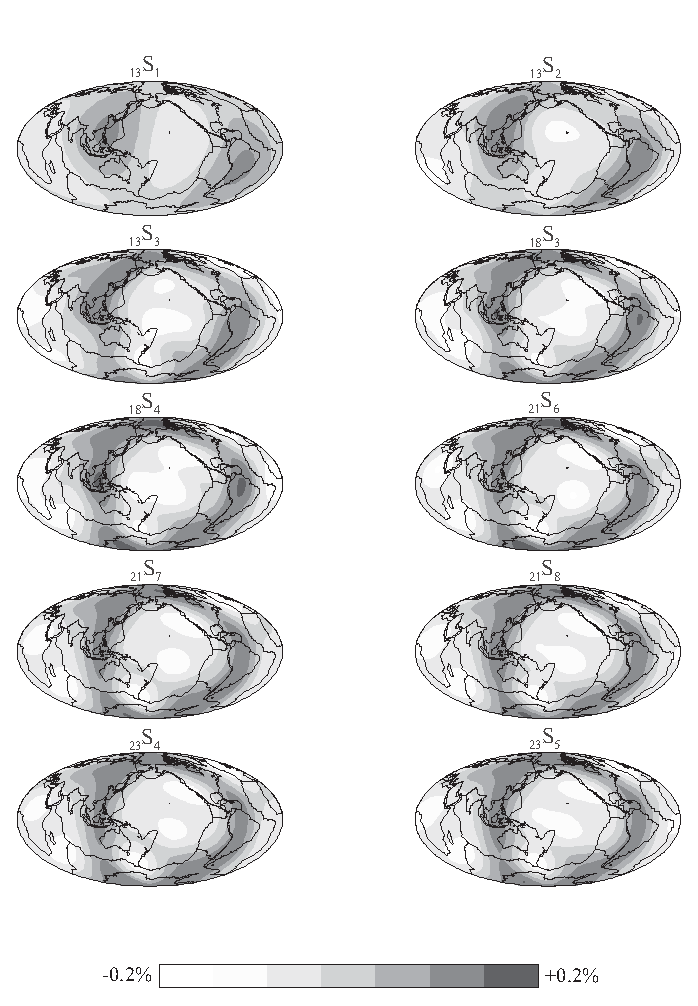
\includegraphics{../figures/chap14/fig14.eps}
}
\end{center}
\caption[core_splittingfunction_pred]{\label{fig:14.core_splittingfunction_pred}
\iffalse
Predicted splitting functions $\sigma^{\rm pre}$ of the eight
spheroidal multiplets in Figure~\protect\ref{fig:14.core_splittingfunction}.
Model SKS12WM13 of Dziewonski, Liu \& Su (\citeyear{liu&dziewonski96})
has been used to perform the calculations.
The poor agreement between
$\sigma^{\rm obs}$ and $\sigma^{\rm pre}$ is the reason for
the appellation ``anomalously split modes''.
Both the observed
and predicted splitting functions have been been truncated,
with only the three lowest even degrees $s=2,4,6$ retained.
\fi
%%%
图~\protect\ref{fig:14.core_splittingfunction}~中~8~个球型多重态的预测分裂函数~$\sigma^{\rm pre}$。采用~Dziewonski, Liu \& Su~(\citeyear{liu&dziewonski96})~的~SKS12WM13~模型进行计算。$\sigma^{\rm obs}$~和~$\sigma^{\rm pre}$~之间较差的一致性是所谓的“异常分裂模式”的原因。观测和预测分裂函数均已被截断,只保留三个最低偶数阶~$s=2,4,6$。
%%%
}
\end{figure}

\iffalse
Current models of the lateral heterogeneity of the
Earth's mantle agree remarkably well with the splitting
functions of all of the mantle-sensitive spheroidal
and toroidal modes.  To illustrate this, we
compare the observed and predicted variations
$\sigma^{\rm obs}$ and $\sigma^{\rm pre}$ along
the fifth spheroidal-overtone branch ${}_5{\rm S}_l$
in Figures~\ref{fig:14.5Ssplittingfunction}
and~Figure~\ref{fig:14.5Ssplittingfunction_pred}.
The predicted splitting functions are those of the
three-dimensional mantle model SKS12WM13 (Dziewonski, Liu \& Su
\citeyear{liu&dziewonski96}).  This model of the variations in
shear-wave speed $\delta\hspace{-0.2 mm}\beta$ was obtained by
inverting a large collection of absolute and differential
body-wave travel-time and phase-delay observations; no overt
normal-mode data were used in its construction.  The good
agreement between $\sigma^{\rm obs}$ and $\sigma^{\rm pre}$
for these and many other mantle-sensitive modes is indicative of
the robustness of our current understanding of large-scale mantle
heterogeneity. The collection of available mantle-sensitive
splitting functions may be used to constrain three-dimensional
Earth structure. 
\fi
%%%
地幔横向不均匀性目前的模型与所有地幔敏感的球型和环型模式的分裂函数较为一致。为说明这一点,我们在图~\ref{fig:14.5Ssplittingfunction}~和~\ref{fig:14.5Ssplittingfunction_pred}~中比较了五阶球型泛音分支~${}_5{\rm S}_l$~的观测变化~$\sigma^{\rm obs}$~和预测变化~$\sigma^{\rm pre}$。预测的分裂函数是基于三维地幔模型~SKS12WM13(Dziewonski, Liu \& Su \citeyear{liu&dziewonski96})。剪切波速度变化~$\delta\hspace{-0.2 mm}\beta$~模型是通过大量的体波走时和相位延迟观测绝对值和差值反演得到的;其构建未采用公开的简正模式数据。这些模式和许多其他地幔敏感模式的~$\sigma^{\rm obs}$~和~$\sigma^{\rm pre}$~具有良好一致性,这表明我们目前对大尺度地幔不均匀性的认知较为可靠。目前可用的地幔敏感分裂函数集可用于约束三维地球结构。
%%%

\iffalse
The core-sensitive spheroidal oscillations displayed
in Figure~\ref{fig:14.core_splittingfunction} are characterized
by very different---predominantly $\sY_{20}$---splitting
functions $\sigma^{\rm obs}$.  These observations are completely
inconsistent with the predominantly $\sY_{2\,\pm 2}$ predictions
$\sigma^{\rm pre}$ of model SKS12WM13, shown in
Figure~\ref{fig:14.core_splittingfunction_pred}.
In fact, these modes are primarily split by
the transverse isotropy of the solid inner core,
as we have seen in Section~\ref{14.sec.incsplit}.
The splitting functions $\sigma^{\rm obs}$ of
such anomalously split multiplets can be measured
by fitting coefficients $\sigma_{st}$ to a suite
of spectra~(\ref{14.myaom}); however, these
coefficients cannot be interpreted strictly in terms
of isotropic heterogeneity $\delta\hspace{-0.1 mm}\kappa_{st}$,
$\delta\hspace{-0.2 mm}\mu_{st}$, $\delta\hspace{-0.2 mm}\rho_{st}$,
$\delta\hspace{-0.1 mm}d_{st}$ using equation~(\ref{eq:14.cst}).
It is a straightforward matter to incorporate {\em both\/} inner-core
anisotropy and isotropic mantle heterogeneity into the spectral-fitting
procedure; the splitting matrix in equation~(\ref{14.myaom})
must be replaced by $\ssH\rightarrow\ssH+(2\om_0)^{-1}\ssV^{\rm ani}$.
Every multiplet then has three more unknowns that are available to
be adjusted in the fitting---the anisotropic coefficients $a'$, $c'$
and $d$ in~(\ref{14.aaniso})--(\ref{14.daniso}).
\index{splitting function|)}%
\index{spectral fitting|)}%
\fi
%%%
图~\ref{fig:14.core_splittingfunction}~中的核敏感球型振荡由非常不同的分裂函数~$\sigma^{\rm obs}$(以~$\sY_{20}$~为主)表征。如图~\ref{fig:14.core_splittingfunction_pred}~所示,这些观测结果与以~$\sY_{2\,\pm 2}$~为主的~SKS12WM13~模型预测结果~$\sigma^{\rm pre}$~完全不一致。事实上,这些模式分裂主要是由固态内核的横向各向同性所致(见~\ref{14.sec.incsplit}~节)。这种异常分裂多重态的分裂函数~$\sigma^{\rm obs}$~可通过将系数~$\sigma_{st}$~拟合至一组观测谱~(\ref{14.myaom})~而获得;然而,这些系数不能利用(14.77)式的各向同性不均匀性~$\delta\hspace{-0.1 mm}\kappa_{st}$、$\delta\hspace{-0.2 mm}\mu_{st}$、$\delta\hspace{-0.2 mm}\rho_{st}$、$\delta\hspace{-0.1 mm}d_{st}$~来严格解释。将内核各向异性和各向同性地幔的不均匀性纳入频谱拟合过程中是一件简单的事情;(\ref{14.myaom})~式中的分裂矩阵必须被替换:$\ssH\rightarrow\ssH+(2\om_0)^{-1}\ssV^{\rm ani}$。如此,任一多重态都有三个未知量可供在拟合时调整,即公式~(\ref{14.aaniso})--(\ref{14.daniso})~中的各向异性系数~$a'$、$a'$~和~$d$。
%%%

\renewcommand{\thesubsection}{$\!\!\!\raise1.3ex\hbox{$\star$}\!\!$
\arabic{chapter}.\arabic{section}.\arabic{subsection}}
%\subsection{Peak shifts}
\subsection{峰值偏移}
\index{peak shifts|(}%
\renewcommand{\thesubsection}{\arabic{chapter}.\arabic{section}.\arabic{subsection}}

\iffalse
Many of the Earth's intermediate-frequency free oscillations exhibit
unresolvably split spectra that may be well fit by a
single Lorentzian; however, the peak locations are often
systematically shifted with respect to the PREM model,
as illustrated in Figure~14.15.
The observed spectral peaks of mode ${}_0{\rm S}_{6}$
at stations ALE in
Alert, Northwest Territories, Canada
and KIP in Kipapa, Hawaii, following the great 1994 Bolivia earthquake, are obviously quite
``singlet-like''.  The coincidence of the ALE peak
with the degenerate PREM frequency
is an indication that the average mantle shear-wave speed underlying the
Bolivia-Alert great-circle path is similar to that of PREM.
The low-frequency shift of the KIP peak indicates, on the
other hand, that the average speed beneath
the Bolivia-Kipapa path is slower than that of PREM.  
We discuss this {\em path-dependent peak-shift\/}
phenomenon in this section.  As a measure of the
location of a spectral peak, we use the real {\em centroid\/}
\index{centroid}%
$\om_{\star}$ of the spectrum $a(\om)$, defined by
\fi
%%%
很多地球中频自由振荡表现出无法分辨的分裂谱,后者可被单一的洛伦兹函数较好地拟合;然而,如图~14.15~所示,峰值位置相对于~PREM~模型经常发生系统性偏移。1994~年玻利维亚大地震后,加拿大西北地区~Alert~的~ALE~台站和夏威夷~Kipapa~的~KIP~台站的~${}_0{\rm S}_{6}$~模式观测谱峰明显是“似单态”的。ALE~峰值与~PREM~简并频率的一致性表明,Bolivia--Alert~大圆路径下的平均地幔剪切波速度与~PREM~模型相应参数相似。另一方面,KIP~峰值的低频偏移表明,Bolivia--Kipapa~路径下的平均地幔剪切波速度慢于~PREM~模型相应参数。在本节中,我们将讨论这种路径依赖的峰值偏移现象。为测量峰值位置,我们采用频谱~$a(\om)$~的实数中心频率~$\om_{\star}$,定义其为
%%%
\eq \label{14.re}
\real\int_0^{\infty}(\om-\omega_{\star})a(\om)\,d\om=0.
\en
\iffalse
The {\em shift\/} in the peak location relative
to the reference degenerate frequency $\om_0$ is the difference
$\delta\om_{\star}=\om_{\star}-\om_0$.
We seek an asymptotic representation
of $\delta\om_{\star}$ valid in the limit
of {\em smooth\/} lateral heterogeneity, $s_{\rm max} \ll l$.
\fi
%%%
式中,$\om_0$~表示峰值位置相对于参考简并频率~$\delta\om_{\star}=\om_{\star}-\om_0$~的偏移;在平滑横向不均匀性~$s_{\rm max} \ll l$~的限制下,采用一个合理的渐近形式表示~$\delta\om_{\star}$。
%%%
\begin{figure}[!t]
\centering
\begin{tabular}{lr}
\begin{tabular}{l}
\scalebox{0.75}{
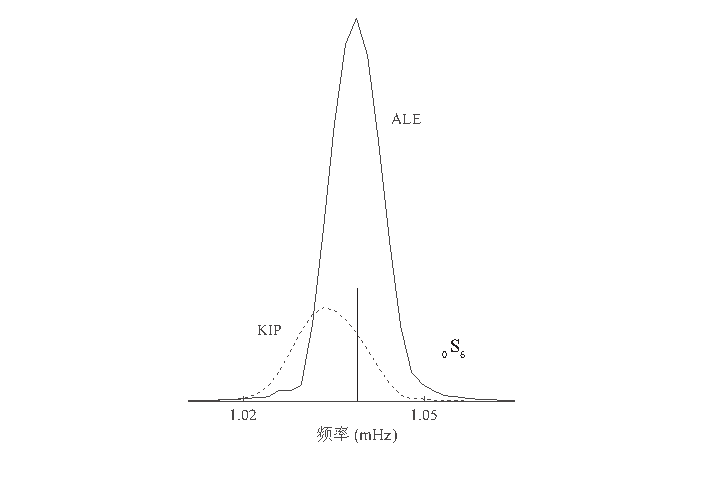
\includegraphics{../figures/chap14/fig15.eps}
}
\end{tabular}
&
\hspace{0.1cm}
\parbox{5.0cm}{\small
Figure~14.15. 
\iffalse
Radial-component amplitude spectra
$|\hat{\bf r}\cdot{\bf a}({\bf x},\omega)|$
of the ${}_{0}{\rm S}_6$ multiplet at stations ALE in
Alert, Canada ({\em solid curve\/})
and KIP in Kipapa, Hawaii ({\em dashed curve\/}), following
the June 9, 1994 deep-focus earthquake in Bolivia.
Vertical line denotes the degenerate PREM
eigenfrequency.
\fi
%%%
1994~年~6~月~9~日玻利维亚深源地震后,加拿大~Alert~的~ALE~台站(实线)和夏威夷~Kipapa~的~KIP~台站(虚线)的~${}_{0}{\rm S}_6$~多重态的径向分量振幅谱~$|\hat{\bf r}\cdot{\bf a}({\bf x},\omega)|$。垂线表示~PREM~模型的简并本征频率。
%%%
}
\end{tabular}
\end{figure}
\addtocounter{figure}{1}

\iffalse
To simplify matters, we ignore the rotation and aspherical anelasticity
of the Earth; in addition, we ignore the renormalization of the singlet
eigenfunctions, and treat the ellipticity as simply the hydrostatic part
of the degree-two perturbation $\delta\hspace{-0.1 mm}\kappa_{20}$,
$\delta\hspace{-0.2 mm}\mu_{20}$, $\delta\hspace{-0.2 mm}\rho_{20}$,
$\delta\hspace{-0.1 mm}d_{20}$.  The splitting matrix~(\ref{14.HSELF})
may then be written, using an obvious notation, in the form
\fi
%%%
为简化问题,我们忽略了地球的自转和非球面非弹性;此外,我们还忽略了单态本征函数的重归一化,将椭率简单地视为二阶微扰~$\delta\hspace{-0.1 mm}\kappa_{20}$、$\delta\hspace{-0.2 mm}\mu_{20}$、$\delta\hspace{-0.2 mm}\rho_{20}$~和~$\delta\hspace{-0.1 mm}d_{20}$~的流体静力学部分。分裂矩阵~(\ref{14.HSELF})~可采用如下的显示表达形式
%%%
\eq \label{14.Lambda}
\ssH=\ssV^{\rm ell+lat}-\om_0^2\ssT^{\rm ell+lat}.
\en
\iffalse
Since~(\ref{14.Lambda}) is real and symmetric it may be
diagonalized by an orthogonal transformation: $\ssZ^{\rm T}\ssZ=\ssI$
and $\ssZ^{\rm T}\ssH\ssZ=\ssDelta$ where $\ssDelta={\rm diag}\,
[\,\cdots\delta\om_j\cdots\,]$.  The spectrum of an isolated multiplet
may be written in terms of the transformed receiver and source vectors
$\ssr'=\ssZ^{\rm T}\ssr$ and $\sss'=\ssZ^{\rm T}\sss$ in the form
\fi
%%%
由于式~(\ref{14.Lambda})~是实数且对称的,因此可通过~$\ssZ^{\rm T}\ssZ=\ssI$~和~$\ssZ^{\rm T}\ssH\ssZ=\ssDelta$~的正交变换对其进行对角化,其中~$\ssDelta={\rm diag}\,
[\,\cdots\delta\om_j\cdots\,]$。孤立多重态的频谱可以写成变换后的接收点和震源向量~$\ssr'=\ssZ^{\rm T}\ssr$~和~$\ssr'=\ssZ^{\rm T}\ssr$~的形式
%%%
\eq \label{14.myaom2}
a(\omega)=\half i\ssr^{\prime_{\,}\rm T}
[\ssDelta-(\omega-\omega_0-i\gamma_0)\ssI]^{-1}\sss'
=\sum_jA_j\eta_j(\om),
\en
\iffalse
where
\fi
%%%
其中,
%%%
\eq \label{14.Ajfull}
A_j=r_j^{\prime}s_j^{\prime}=\left(\sum_mZ_{mj}r_m\right)
\left(\sum_mZ_{mj}s_m\right).
\en
\iffalse
Upon substituting~(\ref{14.myaom2})--(\ref{14.Ajfull})
into equation~(\ref{14.re}) we find that the centroid shift
$\delta\om_{\star}$ is given by
\fi
%%%
将~(\ref{14.myaom2})--(\ref{14.Ajfull})~式代入~(\ref{14.re})~式中,则中心频率偏移~$\delta\om_{\star}$~可表示为
%%%
\eq \label{14.dwapp1}
\delta\omega_{\star}=\frac{\sum_j\delta\om_jA_j}{\sum_jA_j}
=\frac{\ssr^{\rm T}\ssH\sss}{\ssr^{\rm T}\sss}.
\en
\iffalse
The first equality in~(\ref{14.dwapp1}) is intuitively
obvious---every unit Lorentzian in~(\ref{14.myaom2}) has the same area
$\int_0^\infty\eta_j(\om)\,d\om=\pi/2$; the centroid
of $2l+1$ weighted peaks is therefore the centroid
of their centers.  The elements of the splitting
matrix~(\ref{14.Lambda}) are given by
\fi
%%%
(\ref{14.dwapp1})~式中的第一个等式直观上是显而易见的,式~(\ref{14.myaom2})~式中的每个单位洛伦兹函数都有相同的面积~$\int_0^\infty\eta_j(\om)\,d\om=\pi/2$;因此,$2l+1$~个加权峰值的中心就是它们中点的中心。分裂矩阵~(\ref{14.Lambda})~的元素可表示为
%%%
\eqa \label{14.Lambda2} \lefteqn{
H_{mm'}=\frac{1}{2\omega_0}\sum_{st}\biggl\{\int_0^a
[\delta\hspace{-0.1mm}\kappa_{st}V_\kappa+\delta\hspace{-0.2mm}\mu_{st}V_\mu
+\delta\hspace{-0.2mm}\rho_{st}(V_\rho-\omega_0^2T_\rho)]\,r^2dr
} \nonumber \\
&&\mbox{}
+\sum_d d^2\delta\hspace{-0.1mm}d_{st}[V_d-\omega_0^2T_d]_-^+\biggr\}
\int_{\Omega}\sY_{lm}\sY_{st}\sY_{lm'}\,d\Omega.
\ena
\iffalse
Correct to order $(s/l)^2$ we may replace the radial kernels
in~(\ref{14.Lambda2}) by those governing a spherically
symmetric ($s=0$) perturbation:
\fi
%%%
精确至~$(s/l)^2$~阶,可采用控制球对称($s=0$)微扰的核函数来代替式~(\ref{14.Lambda2})~中的径向核函数:
%%%
\eq \label{14.locapp1}
V_\kappa\approx V_{\kappa}^{s=0},\qquad
V_\mu\approx V_{\mu}^{s=0},\qquad
V_{\rho}\approx V_{\rho}^{s=0},
\en
\eq \label{14.locapp2}
T_{\rho}\approx T_{\rho}^{s=0},\qquad
V_d\approx V_d^{s=0},\qquad
T_d\approx T_d^{s=0}.
\en
\iffalse
It is convenient to introduce a {\em local\/}
eigenfrequency perturbation, defined at every
\index{local eigenfrequency}%
\index{eigenfrequency!local}%
point $\theta,\phi$ on the Earth's surface by
\fi
%%%
引入局地本征频率微扰,定义其在地表任意一点~$\theta,\phi$~处为
%%%
\eq \label{14.wlocal}
\delta\om(\theta,\phi)=\sum_{s,t}\delta\om_{st}
\sY_{st}(\theta,\phi),
\en
\iffalse
where
\fi
%%%
其中,
%%%
\eqa \label{14.wlocal2} \lefteqn{
\delta\om_{st}=\frac{1}{2\omega_0}\biggl\{\int_0^a
[\delta\hspace{-0.1mm}\kappa_{st}V_\kappa^{s=0}+\delta\hspace{-0.2mm}\mu_{st}V_\mu^{s=0}
+\delta\hspace{-0.2mm}\rho_{st}(V_\rho^{s=0}-\omega_0^2T_\rho^{s=0})]\,r^2dr
} \nonumber \\
&&\mbox{}
+\sum_d d^2\delta\hspace{-0.1mm}d_{st}[V_d^{s=0}-\omega_0^2T_d^{s=0}]_-^+\biggr\}.
\ena
\iffalse
The quantity $\delta\om(\theta,\phi)$
has a simple physical interpretation---it is the
perturbation to $\om_0$ that would result
if the entire Earth were to suffer a
{\em spherically symmetric\/} perturbation
identical to that beneath the point $\theta,\phi$.
The approximations~(\ref{14.locapp1})--(\ref{14.locapp2})
allow us to write the elements~(\ref{14.Lambda2}) of $\ssH$
in terms of this local eigenfrequency perturbation in the form
\fi
%%%
物理量~$\delta\om(\theta,\phi)$~有一个简单的物理解释,即如果整个地球遭受与~$\theta,\phi$~点以下部分相同的球对称微扰,就会导致对~$\om_0$~的微扰。根据近似关系~(\ref{14.locapp1})--(\ref{14.locapp2}),可将~$\ssH$~的元素~(\ref{14.Lambda2})~用该局地本征频率微扰写成如下形式
%%%
\eq \label{14.Lambdapp}
H_{mm'}\approx\int_\Omega\sY_{lm}\hspace{0.3 mm}
\delta\omega\hspace{0.3 mm}\sY_{lm'}\,d\Omega.
\en
\iffalse
Upon substituting~(\ref{14.Lambdapp}) into equation~(\ref{14.dwapp1})
and using the spherical-harmonic addition theorem~(\ref{B.realaddth})
three times, we obtain the result
\fi
%%%
将式~(\ref{14.Lambdapp})~代入~(\ref{14.dwapp1})~中,并三次利用球谐函数叠加定理~(\ref{B.realaddth}),可得到如下结果
%%%
\eqa \label{14.step2} \lefteqn{
\delta\omega_{\star}\,(\bnuh\cdot\bD)(\bM\!:\!\bE_{\rm s})
\,X_{l0}(\Theta)} \\
&&\mbox{}=\sqrt{\frac{2l+1}{4\pi}}
\,(\bnuh\cdot\bD)(\bM\!:\!\bE_{\rm s})
\int_\Omega X_{l0}(\Theta_{\rm r})\hspace{0.3 mm}
\delta\omega\hspace{0.3 mm} 
X_{l0}(\Theta_{\rm s})\,d\Omega. \nonumber
\ena
\iffalse
Here $\Theta$ denotes the epicentral distance between
the source and the receiver, $\Theta_{\rm r}$ denotes
the angular distance between the integration point and
the receiver, and $\Theta_{\rm s}$ denotes the angular
distance between the integration point and the source.
The symbols $\bD$ and $\bE_{\rm s}$ denote the receiver
displacement and source strain operators~(\ref{14.dispOp})
and~(\ref{14.strainOp}).  For high-degree modes the
zonal spherical harmonic $X_{l0}$ may be approximated
by the asymptotic representation~(\ref{B.Xlpetitm2}).
The method of stationary phase may then be used to
evaluate the surface integral in equation~(\ref{14.step2}).
Retaining terms of order $k^{-1}$, we find
\fi
%%%
其中,$\Theta$~为震源与接收点之间的震中距,$\Theta_{\rm r}$~为积分点与接收点之间的角距,$\Theta_{\rm s}$~为积分点与震源之间的角距。符号~$\bD$~和~$\bE_{\rm s}$~分别表示接收点位移算子~(\ref{14.dispOp})~和震源应变算子~(\ref{14.strainOp})。对于高阶模式,带状球谐函数~$X_{l0}$~可以用渐近形式~(\ref{B.Xlpetitm2})~来近似表示,然后利用稳定相位法来计算式~(\ref{14.step2})~中的曲面积分。保留级数~$k^{-1}$~项,可知
%%%
\eqa \label{14.RomRou}
\lefteqn{
\int_\Omega X_{l0}(\Theta_{\rm r})
\hspace{0.3 mm}\delta\omega\hspace{0.3 mm}
X_{l0}(\Theta_{\rm s})\,d\Omega} \nonumber \\
&&\mbox{}
\approx\invpi(\sin\Theta)^{-1/2}\big[\dombar\cos(k\Theta-\pi/4)
\nonumber \\
&&\mbox{}\qquad
+\half k^{-1}(\cot\Theta\,\p^2_{\ophi}\dombar
-\p_\otheta\p_\ophi\dombar)\sin(k\Theta-\pi/4)
\nonumber \\
&&\mbox{}\qquad
+\eighth k^{-1}\dombar\cot\Theta\sin(k\Theta-\pi/4)\big].
\ena
\iffalse
The quantities $\bar{\theta}$ and $\bar{\phi}$ are
the coordinates of the {\em positive pole of the
source-receiver great circle\/}, and
\fi
%%%
式中,$\bar{\theta}$~和~$\bar{\phi}$~是震源--接收点大圆的正极点;$\dombar$~是局地本征频率微扰的大圆平均值
%%%
\eq \label{14.dombar}
\dombar(\otheta,\ophi)=
\frac{1}{2\pi}\oint_{\otheta,\ophi}\delta\omega(\theta,\phi)
\,d\/\Delta
\en
\iffalse
is the {\em great-circular average\/} of
\index{great-circular average}%
the local eigenfrequency perturbation.
All that remains is to let the operator product
$(\bnuh\cdot\bD)(\bM\!:\!\bE_{\rm s})$ act upon
the expression~(\ref{14.RomRou}). 
Correct to order $k^{-1}$, for either a spheroidal mode observed
on the radial component or a toroidal mode observed on
the transverse component, we obtain
\fi
%%%
\textcolor{red}{剩下的就是让算子积~$(\bnuh\cdot\bD)(\bM\!:\!\bE_{\rm s})$~作用于~(\ref{14.RomRou})~式}。精确至~$k^{-1}$~量级,对于在径向分量观测到的球型模式或在横向分量观测到的环型模式,可得到
%%%
\eqa \label{14.RomRou2}
\lefteqn{
\delta\omega_{\star}\approx\dombar+k^{-1}(\sin\Theta)^{-1}\Big\{
x(\cos\Theta\,\p_\ophi\dombar-\sin\Theta\,\p_\otheta\dombar)}
\nonumber \\
&&\mbox{}
\qquad\qquad+\big[\half(\cos\Theta\,\p^2_\ophi\dombar-
\sin\Theta\,\p_\otheta\p_\ophi\dombar) \nonumber \\
&&\mbox{}
\qquad\qquad+y(\cos\Theta\,\p_\ophi\dombar-
\sin\Theta\,\p_\otheta\dombar)\big]
\nonumber \\
&&\mbox{}\qquad\qquad\times
\tan(k\Theta-\pi/4+z)\Big\},
\ena
\iffalse
where
\fi
%%%
其中,
%%%
\eq
x=\frac{(\Sigma_0-\Sigma_2)\p_\ophi\Sigma_1+\Sigma_1\p_\ophi\Sigma_2}
{(\Sigma_0-\Sigma_2)^2+\Sigma_1^2},
\en
\eq
y=\frac{\Sigma_1\p_\ophi\Sigma_1-(\Sigma_0-\Sigma_2)\p_\ophi\Sigma_2}
{(\Sigma_0-\Sigma_2)^2+\Sigma_1^2},
\en
\eq
z=\left\{\begin{array}{ll}
\displaystyle{\arctan\left(\frac{\Sigma_1}{\Sigma_0-\Sigma_2}\right)} &
\mbox{for a spheroidal mode} \\
\vspace{-0.5 mm} & \vspace{-0.5 mm} \\
\displaystyle{\arctan\left(\frac{\p_\ophi\Sigma_1}{\Sigma_1}\right)} &
\mbox{for a toroidal mode.}
\end{array} \right.
\en
\iffalse
The quantities $\Sigma_m(\bar{\phi})$, $m=0,1,2$ are defined
in terms of the moment-tensor excitation
coefficients~(\ref{10.isorad})--(\ref{10.B2need}) by
\fi
%%%
量~$\Sigma_m(\bar{\phi})$, $m=0,1,2$~由矩张量激发系数~(\ref{10.isorad})--(\ref{10.B2need})~定义为
%%%
\eq
\Sigma_m=(-1)^m
%\left(\frac{4\pi}{2l+1}\right)^{1/2}
\left[\frac{(l+m)!}{(l-m)!}\right]^{1/2}
(A_m\cos m\ophi+B_m\sin m\ophi).
\en
\iffalse
The above order $k^{-1}$ analysis is due to Davis \& Henson
(\citeyear{davis&henson86}) and Romanowicz \& Roult
(\citeyear{romanowicz&roult86}); the more suggestive lowest-order
result
\fi
%%%
以上~$k^{-1}$~量级分析来自于Davis \& Henson~(\citeyear{davis&henson86})~和~Romanowicz \& Roult~(\citeyear{romanowicz&roult86});更具启示性的最低阶结果则更早由~Jordan~(\citeyear{jordan78})~和~Dahlen~(\citeyear{dahlen79})~推导,即
%%%
\eq \label{14.TOM}
\delta\omega_{\star}\approx\frac{1}{2\pi}\oint_{\otheta,\ophi}
\delta\omega(\theta,\phi)
\,d\/\Delta
\en
\iffalse
was derived somewhat earlier by Jordan (\citeyear{jordan78})
and Dahlen (\citeyear{dahlen79}).  The asymptotic influence of along-branch
multiplet coupling has been considered by Park (\citeyear{park87})
and Romanowicz (\citeyear{romanowicz87}).
\fi
%%%
同阶多重态耦合的渐近影响已被~Park~(\citeyear{park87})~和~Romanowicz~(\citeyear{romanowicz87})~考虑。
%%%

\iffalse
Equation~(\ref{14.TOM})
stipulates that the asymptotic location $\om_0+\delta\om_{\star}$
of a peak depends only upon the average structure immediately
underlying the source-receiver great-circle path.
The mechanism responsible for the ``singlet-like'' appearance
of the superposition~(\ref{14.myaom2}) of $2l+1$ closely spaced
resonance peaks is mode-mode interference.
The amplitudes~(\ref{14.Ajfull}) of the constituent Lorentzians
are all real; however, the signs ${\rm sgn}\,A_j$ alternate
between $\pm 1$.  Singlets with eigenfrequency perturbations
$\delta\om_j$ in the vicinity of $\delta\om_{\star}$ tend to be
strongly excited and of the same sign, so that they interfere constructively,
whereas all other singlets are either weakly excited or interfere
destructively.  Dahlen (\citeyear{dahlen79b}) and Davis \& Henson
(\citeyear{davis&henson86}) present a number of synthetic examples
that illustrate this singlet interference ``in action''.
\fi
%%%
(\ref{14.TOM})~式规定,某一峰值的渐近位置~$\om_0+\delta\om_{\star}$~仅取决于震源--接收点大圆路径下的平均结构。$2l+1$~个密集共振峰叠加~(\ref{14.myaom2})~式所呈现的“似单态”的机制响应是模式间的干扰。构成洛伦兹函数的振幅~(\ref{14.Ajfull})~均是实数的;然而,符号~${\rm sgn}\,A_j$~在~$\pm 1$~之间交替变化。在~$\delta\om_{\star}$~附近具有本征频率微扰~$\delta\om_j$~的单态模式往往是被强激发的,并且具有相同的符号,因此它们相长干扰,而所有其他单态模式要么是被弱激发的,要么是相消干扰的。Dahlen~(\citeyear{dahlen79b})~和~Davis \& Henson~(\citeyear{davis&henson86})~举出了一些合成例子来说明这种单态模式干扰“作用”。
%%%

\iffalse
Upon making use of the Roberts-Ursell-Backus identity~(\ref{B.Ylmoint}),
we may write the spherical-harmonic representation of~(\ref{14.TOM})
in the form
\fi
%%%
利用~Roberts--Ursel--Backus~恒等式~(\ref{B.Ylmoint}),我们可将~(\ref{14.TOM})~式的球谐表示写成如下形式
%%%
\eq \label{14.TOM2}
\delta\omega_{\star}\approx
\sum_{\textstyle{{s=2}\atop{s\,\rm even}}}^{2l}\sum_{t=-s}^s
\delta\omega_{st}P_s(0)\sY_{st}(\otheta,\ophi).
\en
\iffalse
The expansion is limited to {\em even\/} degrees $s=2,4,\ldots,2l$
by virtue of the fact that $P_s(0)=0$ whenever $s$ is odd.
Equation (\ref{14.TOM2}) constitutes a linear inverse problem:
peak-shift measurements $\delta\omega_{\star}$ may be used
to determine the expansion coefficients
$\delta\omega_{st}$, $s=2,4,\ldots,2l$.
The coefficients are in turn linearly related to
the even-degree perturbations $\delta\hspace{-0.2 mm}\rho_{st}$,
$\delta\hspace{-0.1 mm}\kappa_{st}$, $\delta\hspace{-0.2 mm}
\mu_{st}$, $\delta\hspace{-0.1 mm}d_{st}$ by equation~(\ref{14.wlocal2}).
The selection rules~(\ref{14.selrule}) suggest that it
should be possible to write the asymptotic splitting
matrix in a manner that reflects its dependence
only upon the even degrees $s$; in fact,
the complex elements
$\tilde{H}_{mm'}\approx\int_{\Omega}Y_{lm}^*
\delta\omega\hspace{0.3 mm}Y_{lm'}\,d\Omega$
of the transformed matrix~$\tilde{\ssH}$
are given by
\fi
%%%
由于当~$s$~为奇数时,$P_s(0)=0$,因此该展开式被限制于偶数阶~$s=2,4,\ldots,2l$。式~(\ref{14.TOM2})~构成了一个线性反演问题:峰值偏移观测量~$\delta\omega_{\star}$~可用于确定膨胀系数~$\delta\omega_{st}$, $s=2,4,\ldots,2l$。根据式~(\ref{14.wlocal2}),这些系数依次与偶数阶微扰~$\delta\hspace{-0.2 mm}\rho_{st}$、$\delta\hspace{-0.1 mm}\kappa_{st}$、$\delta\hspace{-0.2 mm}
\mu_{st}$~和~$\delta\hspace{-0.1 mm}d_{st}$~呈线性相关。根据选择法则~(\ref{14.selrule}),可将渐近分裂矩阵写成只依赖于偶数阶~$s$~的形式;实际上,变换矩阵~$\tilde{\ssH}$~的复数元素~$\tilde{H}_{mm'}\approx\int_{\Omega}Y_{lm}^*
\delta\omega\hspace{0.3 mm}Y_{lm'}\,d\Omega$~可表示为
%%%
\eq \label{14.Lambdapp2}
\tilde{H}_{mm'}\approx\frac{1}{2\pi}\int_0^{2\pi}
\delta\bar{\om}(\bar{\theta},\bar{\phi})
e^{-i(m-m')\bar{\phi}}\,d\bar{\phi},
\en
\iffalse
where
\fi
%%%
其中,
%%%
\eq \label{14.Lambdapp3}
\cos\bar{\theta}=\frac{m+m'}{2l+1}.
\en
\iffalse
The result~(\ref{14.Lambdapp2})--(\ref{14.Lambdapp3})
follows from~(\ref{14.Lambdapp})
upon application of the Gaunt-integral asymptotic
relation~(\ref{C.asymp5}).
\fi
%%%
利用冈特积分渐近关系~(\ref{C.asymp5})~可得式~(\ref{14.Lambdapp})~的结果~(\ref{14.Lambdapp2})--(\ref{14.Lambdapp3})。
%%%

\iffalse
A more refined analysis allows for slow variations in
the location and amplitude of a peak with time.
The starting point in this case is the time-domain
analogue of equation~(\ref{14.myaom2}):
\fi
%%%
若考虑一种更为精细的分析,即允许某一峰值的位置和振幅随时间发生慢变,则首先需要给出~(\ref{14.myaom2})~式的时域模拟:
%%%
\eq \label{14.smimas1}
A_0(t)=\ssr^{\rm T}\exp(i\ssH t)\,\sss.
\en
\iffalse
We can rewrite this multiplet modulation function
without further approximation as a single complex exponential:
\fi
%%%
可将该多重态调制函数改写为一个复指数函数,但不做进一步近似处理,即:
%%%
\eq \label{14.smimas2}
A_0(t)=\ssr^{\rm T}\sss\,\exp
\left[i\int_0^t\delta\om_{\star}(t')\,dt'\right].
\en
\iffalse
The integrand in equation~(\ref{14.smimas2}) is a complex
{\em instantaneous frequency shift\/}
\index{frequency shift}%
given by
\fi
%%%
(\ref{14.smimas2})~式中的被积函数为如下复数瞬时频移
%%%
\eq \label{14.smimas3}
\delta\om_{\star}(t)=\frac{\ssr^{\rm T}
\ssH\exp(i\ssH t)\,\sss}{\ssr^{\rm T}\exp(i\ssH t)\,\sss}.
\en
\iffalse
At the outset, $t=0$, this instantaneous shift
coincides with~(\ref{14.dwapp1}); more generally,
however, we may use~(\ref{14.smimas3}) to express
$\delta\om_{\star}(t)$ as a slowly varying Taylor series:
\fi
%%%
开始时~$t=0$,该瞬时位移与~(\ref{14.dwapp1})~式相符;然而,更一般来说,可用式~(\ref{14.smimas3})~将~$\delta\om_{\star}(t)$~表示为慢变泰勒级数:
%%%
\eq \label{14.smimas4}
\delta\om_{\star}(t)=\delta\om_{\star}
+\delta\om_{\star}^{\prime}t
+\half\delta\om_{\star}^{\prime\prime}t^2
+\cdots,
\en
\iffalse
where
\fi
%%%
其中,
%%%
\eq \label{14.smimas5}
\delta\om_{\star}=\frac{\ssr^{\rm T}\ssH\sss}{\ssr^{\rm T}\sss},
\qquad\delta\om_{\star}^{\prime}=i\left[
\frac{\ssr^{\rm T}\ssH^2\sss}{\ssr^{\rm T}\sss}
-\left(\frac{\ssr^{\rm T}\ssH\sss}{\ssr^{\rm T}\sss}
\right)^2\right],
\en
\eq \label{14.smimas6}
\delta\om_{\star}^{\prime\prime}=-\left[
\frac{\ssr^{\rm T}\ssH^3\sss}{\ssr^{\rm T}\sss}
-\frac{3(\ssr^{\rm T}\ssH\sss)(\ssr^{\rm T}\ssH^2\sss)}
{(\ssr^{\rm T}\sss)^2}+2\left(\frac{\ssr^{\rm T}\ssH\sss}{\ssr^{\rm T}\sss}
\right)^3\right].
\en
\begin{figure}[!b]
\begin{center}
\includegraphics{../figures/chap14/fig16b.eps}
\end{center}
\caption[peakshifts]{\label{fig:14.peakshifts}
\iffalse
Observed peak shifts $\langle\delta\omega_{\star}\rangle$ of the
fundamental spheroidal multiplet ${}_0{\rm S}_{23}$.
Each of the 1400 measurements is plotted twice,
at the two great-circle poles $\bar{\theta},\bar{\phi}$
and $\pi-\bar{\theta},
\pi+\bar{\phi}$.  Plus symbols $\scriptstyle +$
and diamonds $\diamond$ denote positive and negative
shifts, respectively.  The size of each symbol is
proportional to the magnitude of the frequency shift,
with maximum variations of $\pm 10$~$\mu$Hz.
Paths with their poles in the Central Pacific
are shifted to high frequency, because
the shear-wave speed variations underlying the
circum-Pacific are relatively fast.
(Courtesy of R. Widmer.)
\fi
%%%
基阶球型多重态~${}_0{\rm S}_{23}$~的观测峰值偏移~$\langle\delta\omega_{\star}\rangle$。在两个大圆极点~$\bar{\theta},\bar{\phi}$~和~$\pi-\bar{\theta}$、$\pi+\bar{\phi}$~处,1400~次观测被分别绘制一次。加号~$\scriptstyle +$~和菱形符号~$\diamond$~分别表示正偏移和负偏移。每个符号的大小与频移幅度成正比,最大变化为~$\pm 10$~$\mu$~Hz。由于环太平洋区域下的剪切波速度变化相对较快,两极位于太平洋中部的路径被转换为高频。(由~R. Widmer~提供)
%%%
}
\end{figure}
\iffalse
It is found empirically that most ``singlet-like'' peaks
can be adequately fit by a single Lorentzian, without
allowing explicitly for the temporal variations~(\ref{14.smimas4}).
The measured shift in that case is best interpreted as a
weighted average $\langle\delta\omega_{\star}\rangle$
of the instantaneous shift $\delta\om_{\star}(t)$
over the duration of the recording.
The weighting function depends upon the decay rate
$\gamma_0$ as well as the taper used in the analysis.
\fi
%%%
根据经验,在不考虑时间变化~(\ref{14.smimas4})~式的情况下,大多数“似单态”谱峰都可以用一个洛伦兹函数充分拟合。在这种情况下,观测偏移最好解释为记录期间的瞬时偏移~$\delta\om_{\star}(t)$~的加权平均值~$\langle\delta\omega_{\star}\rangle$。该加权函数取决于衰减率~$\gamma_0$~以及分析中使用的窗函数。
%%%

\begin{figure}[!b]
\begin{center}
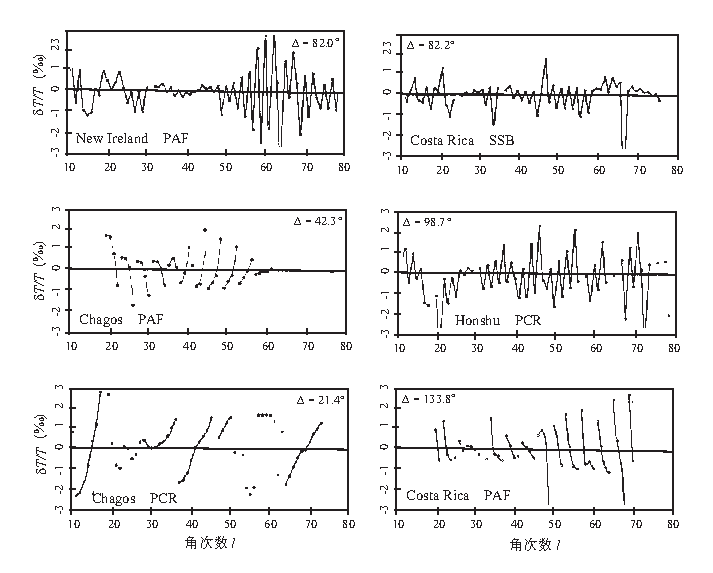
\includegraphics{../figures/chap14/fig17.eps}
\end{center}
\caption[tan]{\label{fig:14.tan}
\iffalse
Fundamental spheroidal-mode peak-shift observations
plotted versus angular degree $l$ for a number of
source-receiver combinations. The smooth $\dombar$
variations have been removed to highlight the
$\tan(k\Theta-\pi/4+z)$ fluctuations.  The
event and station locations and epicentral
distances are indicated in each panel.
Note that the relative perturbation in period $\delta T/T$ is
given in per mille. (Courtesy of B. Romanowicz \& G. Roult.)
\fi
%%%
\textcolor{red}{大量震源--接收点组合},基阶球型模式的峰值偏移观测随角阶次~$l$~的变化。平滑的~$\dombar$~变化已被移除,以突出~$\tan(k\Theta-\pi/4+z)$~波动。每个子图均注明了地震位置、台站位置以及震中距。注意,周期的相对微扰~$\delta T/T$~以千分比为单位。(由~B. Romanowicz \& G. Roult~提供)
%%%
}
\end{figure}
\iffalse
The above procedure was developed and utilized by
Smith \& Masters (\citeyear{smith&masters89})
to update the pioneering peak-shift measurements
of Masters, Jordan, Silver \& Gilbert (\citeyear{masters&al82});
the latter historic analysis provided the first unequivocal
evidence for large-scale upper-mantle lateral heterogeneity,
as we discussed in Section~1.6.  Smith and Masters' last-gasp
analysis fit nearly 3000 spectra, and extracted
1000\hspace{0.6 mm}--\hspace{0.2 mm}1500
 peak shifts $\langle\delta\omega_{\star}\rangle$ for
each of the fundamental spheroidal multiplets
${}_0{\rm S}_{20}\!-\!{}_0{\rm S}_{45}$.
Figure~\ref{fig:14.peakshifts} shows their raw measurements
for mode ${}_0{\rm S}_{23}$
plotted at the poles $\bar{\theta},\bar{\phi}$
of the source-receiver great circles; note the remarkably
coherent degree-two pattern that is visible in the data!
This aspect of the Earth's lateral heterogeneity has been
confirmed---and resolved much more clearly---by numerous
subsequent inversion studies using body and surface waves
as well as normal modes (Masters \citeyear{masters89};
Roult, Romanowicz \& Montagner \citeyear{roult&al90};
Woodward \& Masters \citeyear{woodward&masters91};
Masters, Johnson, Laske \& Bolton \citeyear{masters&al96}).
\fi
%%%
上述程序由~Smith \& Masters~(\citeyear{smith&masters89})~开发和利用,用于更新~Masters, Jordan, Silver \& Gilbert~(\citeyear{masters&al82})~首创的峰值偏移观测;后者的历史分析为上地幔大尺度横向各向异性提供了第一个明确的证据(见~1.6~节)。Smith~和~Masters~最终分析拟合了近~3000~个频谱,并为每一个基阶球型多重态~$\langle\delta\omega_{\star}\rangle$~提取了~1000\hspace{0.6 mm}--\hspace{0.2 mm}1500~个峰值偏移~${}_0{\rm S}_{20}\!-\!{}_0{\rm S}_{45}$。图~\ref{fig:14.peakshifts}~显示了在震源--接收点大圆的极点~$\bar{\theta},\bar{\phi}$~处绘制的~${}_0{\rm S}_{23}$~模式的原始测量值;注意,数据中存在明显的一致的二阶模式!地球的横向不均匀性已经被证实,并通过后续大量使用体波、面波以及简正模式的反演研究得到了更清晰的解决~(Masters \citeyear{masters89};
Roult, Romanowicz \& Montagner \citeyear{roult&al90};
Woodward \& Masters \citeyear{woodward&masters91};
Masters, Johnson, Laske \& Bolton \citeyear{masters&al96})。
%%%

\iffalse
The order $k^{-1}$ terms in~(\ref{14.RomRou2}) constitute
a small correction, except at epicentral distances where
$\tan(k\Theta-\pi/4+z)\rightarrow\pm\infty$, corresponding
to longitudinal {\em nodes\/} of the spherical-Earth
excitation pattern~(\ref{10.vectamp}).  This divergence
gives rise to a degree-dependent fluctuation or jitter
of period $\Delta l\approx\pi/\Theta$ that is superimposed
upon the expected smooth variation of $\delta\om_{\star}$
along a fixed dispersion branch such as ${}_n{\rm S}_l$ or ${}_n{\rm T}_l$.  Such a jitter is a characteristic
feature of fundamental-mode peak-shift data, as illustrated
in Figure~\ref{fig:14.tan}.
The instantaneous frequency shift
$\delta\om_{\star}(t)$ suffers from the same defect, since it is
fundamentally due to the nodal divergence of the denominator
$\ssr^{\rm T}\sss$ in~(\ref{14.dwapp1}).  This same
spherical-Earth excitation amplitude appears in the denominators
of~(\ref{14.smimas5})--(\ref{14.smimas6}); this renders
the expansion~(\ref{14.smimas4}) unsuitable near nodes.
The ubiquity of these nodal
fluctuations and---much more importantly---the insensitivity to
odd-degree structure have led to the gradual abandonment
of ${}_0{\rm S}_l$ and ${}_0{\rm T}_l$  peak-shift measurements.
It is preferable to measure the phase speeds of the equivalent
fundamental-mode surface waves, since these constrain the odd
as well as the even part of the Earth's lateral heterogeneity.
\index{peak shifts|)}%
\fi
%%%
除在震中距~$\tan(k\Theta-\pi/4+z)\rightarrow\pm\infty$~外,式~(\ref{14.RomRou2})~中的~$k^{-1}$~项构成了一个小修正,对应于球对称地球激发模式~(\ref{10.vectamp})~的经向节点。这种发散产生了一个周期为~$\Delta l\approx\pi/\Theta$~的次数依赖性波动或抖动,其会沿固定频散分支(如~${}_n{\rm S}_l$~或~${}_n{\rm T}_l$)叠加在~$\Delta l\approx\pi/\Theta$~的预期平滑变化上。如图~\ref{fig:14.tan}~所示,这种抖动是基阶模式峰值偏移数据的一个特征。瞬时频移~$\delta\om_{\star}(t)$~也有同样的缺陷,因为其本质上是由式~(\ref{14.dwapp1})~中分母~$\ssr^{\rm T}\sss$~的节点散度造成的。同样的球对称地球激发振幅出现在式~(\ref{14.smimas5})--(\ref{14.smimas6})~的分母中;这使得展开式~(\ref{14.smimas4})~不适用于节点附近。这些节点波动普遍存在,更重要的是对奇数阶结构不敏感,导致~${}_0{\rm S}_l$~和~${}_0{\rm T}_l$~峰值偏移观测逐渐被弃用。最好的方式是测量等效基阶模式面波的相速,因为它们可以同时约束地球横向不均匀性的奇数阶和偶数阶部分。
%%%

\renewcommand{\thesubsection}{$\!\!\!\raise1.3ex\hbox{$\star$}\!\!$
\arabic{chapter}.\arabic{section}.\arabic{subsection}}
%\subsection{Spherical stacks}
\subsection{球谐叠加}
\index{stacking|(}%
\renewcommand{\thesubsection}{\arabic{chapter}.\arabic{section}.\arabic{subsection}}

\iffalse
In Section~10.6 we discussed a spectral stacking procedure which
may be used to isolate a target multiplet upon a spherically symmetric
Earth and simultaneously reduce the noise.  We return to this topic
now and ask the question---how does the splitting due to the Earth's
asphericity affect a spherical stack?  An ideal dense-network stack consists
of an integral~(\ref{eq:10.stack}) over the surface of the Earth:
\fi
%%%
在~10.6~节中,我们讨论了一种频谱叠加方法,该方法可用于在球对称地球上分离目标多重态,并降低噪声水平。现在我们回到这一话题,并提出这样一个问题:地球非球面性导致的分裂是如何影响球谐叠加的?理想的密集台网叠加包含一个覆盖地球表面的积分~(\ref{eq:10.stack})~形式:
%%%
\eq \label{14.asphericalstack}
\Sigma(\om)=\int_\Omega\bA(\bx)\cdot\ba(\bx,\om)\,d\Omega,
\en
\iffalse
where $\bA(\bx)$ is the spherical-Earth excitation pattern.
Upon evaluating this surface integral using the split-multiplet
representation~(\ref{14.myaom2})--(\ref{14.Ajfull}) of the
stacked spectra $\ba(\bx,\om)$ we find that
\fi
%%%
式中,$\bA(\bx)$~为球形地球激发样式。通过采用叠加谱~$\ba(\bx,\om)$~的分裂多重态\textcolor{blue}{表达式}~(\ref{14.myaom2})--(\ref{14.Ajfull})~估算该面积分,\textcolor{blue}{可知}
%%%
\eq \label{14.stack}
\Sigma(\om)=\sum_j\sA_j\eta_j(\om),
\en
\iffalse
where
\fi
%%%
其中,
%%%
\eqa \label{14.Ajstack} \lefteqn{
\sA_j=(U_a^2+V_a^2+W_a^2)s_j^{\prime_{\,}2}
=(U_a^2+V_a^2+W_a^2)\left(\sum_{m}Z_{mj}s_m\right)^2.} \nonumber \\
&&\mbox{}
\ena
\begin{figure}[!b]
\begin{center}
\scalebox{1.05}{
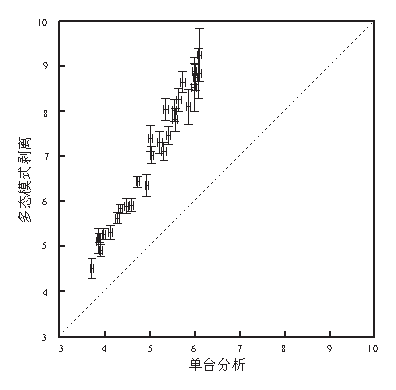
\includegraphics{../figures/chap14/fig18.eps}
}
\end{center}
\caption[Qbias]{\label{fig:14.Qbias}
\iffalse
Scatter plot of $1000\,Q_0^{-1}$ for the fundamental
spheroidal modes ${}_0{\rm S}_l$.  Ordinate shows
measurements made on stripped spherical stacks $\Sigma(\omega)$;
abscissa shows measurements made on single-station
spectra $a(\omega)$.  The latter are not expected
to be severely biased; the stack measurements are
systematically higher, since the spectra $\Sigma(\om)$
are broadened by splitting as well as attenuation.
Error bars denote the $\pm\sigma$ observational uncertainty.
(Courtesy of R. Widmer.)
\fi
%%%
基阶球型模式~${}_0{\rm S}_l$~的~$1000\,Q_0^{-1}$~散点图。纵坐标表示剥离球谐叠加谱~$\Sigma(\omega)$~中的测量值;横坐标表示单台站频谱~$a(\omega)$~中的测量值。后者预计不会有严重偏差;由于叠加谱~$\Sigma(\om)$~是通过分裂和衰减而拓宽的,因此叠加测量值有系统性的提高。误差棒表示观测不确定度~$\pm\sigma$。(由~R. Widmer~提供)
%%%
}
\end{figure}
\iffalse
The subscript $a$ denotes evaluation of the radial
eigenfunctions $U,V,W$ at the receiver radius $r=a$.
An important distinction between the stacked
spectrum~(\ref{14.stack})--(\ref{14.Ajstack}) and a
single-station spectrum~(\ref{14.myaom2})--(\ref{14.Ajfull})
is apparent---the amplitude $\sA_j$ of every singlet
in $\Sigma(\om)$ is {\em positive\/}.  As a result,
there is no destructive interference leading to a
``singlet-like'' peak, as in the case of $a(\om)$;
instead, the interference is purely constructive.
This results in a peak that is significantly wider
than any constituent Lorentzian $\eta_j(\omega)=
\half [\gamma_0+i(\om-\omega_0-\delta\omega_j)]^{-1}$.
Attenuation measurements made on a spherical stack
$\Sigma(\om)$ provide an {\em overestimate\/} $\gamma_{\star}$
of the degenerate decay rate $\gamma_0$ of a multiplet,
for this reason.  Comparisons with single-station
measurements suggest that the resulting bias in
the reciprocal quality factor of the fundamental
spheroidal modes may be as high as forty percent, as
illustrated in~Figure~\ref{fig:14.Qbias}.
The centroid $\om_{\star}$ of a stack also
provides an incorrect estimate of the degenerate
frequency $\om_0$ as a consequence of the non-isotropic
excitation: sectors of the Earth where the dipolar or
quadrupolar excitation pattern $A(\bx)$ is nearly nodal
will be underrepresented (Dahlen \citeyear{dahlen79}).
In this case an obvious bias-reduction strategy
is available---simply include as many events
$\bM$, $\bx_{\rm s}$ in the stack or stacks
$\Sigma(\om)$ as possible.
\index{stacking|)}%
\index{multiplet!isolated|)}%
\index{isolated multiplet|)}%
\fi
%%%
式中,下标~$a$~表示在接收点半径~$r=a$~处估算径向本征函数~$U,V,W$~。叠加谱~(\ref{14.stack})--(\ref{14.Ajstack})~和单台站谱~(\ref{14.myaom2})--(\ref{14.Ajfull})~之间一个重要且明显的区别就是每个单态模式在~$\Sigma(\om)$~中的振幅~$\sA_j$~符号为正。因此,与~$a(\om)$~的情形一样,不存在导致“似单态”谱峰的破坏性干扰;相反,这种干扰是\textcolor{red}{纯}相干的。这导致一个谱峰是显著宽于任意成分的洛伦兹函数~$\eta_j(\omega)=
\half [\gamma_0+i(\om-\omega_0-\delta\omega_j)]^{-1}$。鉴于上述原因,在球谐叠加谱~$\Sigma(\om)$~中进行的衰减测量会给某一多重态的简并衰减率~$\gamma_0$~提供一个高估值~$\gamma_{\star}$。如图~\ref{fig:14.Qbias}~所示,与单台站测量结果的比较表明,基阶球型模式的品质因子倒数的偏差可能高达~40\%。某一叠加的中心频率~$\om_{\star}$~也会给来自非各向同性激发的简并频率~$\om_0$~提供一个错误估值,即地球扇区(两极或四极激发模式~$A(\bx)$~是近节点的)将被低估(Dahlen \citeyear{dahlen79})。在这种情况下,可采用一种显著偏差减少策略,即在叠加或叠加谱~$\Sigma(\om)$~中包含尽可能多的地震事件~$\bM$~和~$\bx_{\rm s}$。
%%%

%\section{Multiplet Coupling}
\section{多重态耦合}
\index{multiplet coupling|(}%
\index{coupled mode|(}%
\index{mode!coupled|(}%

\iffalse
The isolated-multiplet approximation cannot be used to describe
overlapping multiplets, such as the spheroidal-mode pairs
${}_0{\rm S}_7\!-\!{}_2{\rm S}_3$, ${}_1{\rm S}_5\!-\!{}_2{\rm S}_4$
and ${}_2{\rm S}_5\!-\!{}_1{\rm S}_6$ in Figure~\ref{fig:14.lp_spec}.
To account for the possibility of coupling between such pairs,
it is necessary to treat them as a single {\em quasi-degenerate
super-multiplet\/}.
\index{multiplet!super-}% 
\index{super-multiplet}% 
The resulting analysis is computationally more demanding;
however, it has its advantages---as we shall see, super-multiplet
splitting and coupling is sensitive to both even-degree and odd-degree
lateral heterogeneity.
\fi
%%%
孤立多重态近似并不能用于描述重叠多重态,如图~\ref{fig:14.lp_spec}~中的球型模式对~${}_0{\rm S}_7\!-\!{}_2{\rm S}_3$、${}_1{\rm S}_5\!-\!{}_2{\rm S}_4$~和~${}_2{\rm S}_5\!-\!{}_1{\rm S}_6$。为了解释这类模式对之间耦合的可能性,有必要将它们视为单个准简并超级多态模式。这种分析对计算的要求更高;然而,它也有其自身的优点,即正如我们将看到的,超级多态模式分裂和耦合对偶数阶和奇数阶横向不均匀性都很敏感。
%%%

%\subsection{Formalities}
\subsection{\textcolor{red}{形式}}

\iffalse
The splitting and coupling of a super-multiplet
upon a rotating, elliptical, laterally heterogeneous
Earth model is governed by a super-version of the
matrix~(\ref{14.HSELF}):
\fi
%%%
在有旋、椭球、横向不均匀的地球模型中,超级多态模式的分裂和耦合是由矩阵~(\ref{14.HSELF})~的一个超级版本控制,即:
%%%
\eqa \label{14.Htot} \lefteqn{
\ssH=\ssN-\nu_0\ssI+\ssW} \nonumber \\
&&\mbox{}
+(2\om_0)^{-1}[\ssV^{\rm ell+cen}+\ssV^{\rm lat}+i\ssA
-\om_0^2(\ssT^{\rm ell}+\ssT^{\rm lat})].
\ena
\iffalse
The dimension of this matrix is $\sum_k(2l_k+1)\,
\times\,\sum_k(2l_k+1)$, where $l_k$ denotes the
degree of the multiplet $k$. 
The quantity $\nu_0=\om_0+i\gamma_0$ is a
complex fiducial or reference frequency, and
$\ssN={\rm diag}\,[\,\cdots\,\nu_k\,\cdots\,]$
is the diagonal matrix of complex degenerate
eigenfrequencies.  The reference frequency
is arbitrary, but it is typically chosen to be
one of the degenerate frequencies
$\nu_k=\om_k+i\gamma_k$.  The perturbations are
considered to be superimposed upon the anelastic
terrestrial monopole; note that $\ssH$ reduces
to $\ssN-\nu_0\ssI$, so that the degenerate
relative eigenfrequencies $\nu_k-\nu_0$ are
recovered, when rotation, ellipticity and lateral
heterogeneity are ignored.
\fi
%%%
该矩阵的维数为~$l_k$,其中$~\sum_k(2l_k+1)\,
\times\,\sum_k(2l_k+1)$~为多重态~$k$~的次数。$\nu_0=\om_0+i\gamma_0$~表示复基准或参考频率,$\ssN={\rm diag}\,[\,\cdots\,\nu_k\,\cdots\,]$~表示复简并本征频率的对角化矩阵。尽管参考频率是任意的,但通常会选择为其中的一个简并频率~$\nu_k=\om_k+i\gamma_k$。这些微扰被认为是叠加在非弹性地球单极子上的;注意,当忽略自转、椭率和横向不均匀性时,$\ssH$~简化为~$\ssN-\nu_0\ssI$,因此简并相对本征频率~$\nu_k-\nu_0$~被恢复。
%%%

\iffalse
More generally, the diagonal matrix
$\ssDelta={\rm diag}\,[\,\cdots\,\delta\nu_j\,\cdots\,]$
of split singlet eigenfrequencies
$\delta\nu_j=\delta\om_j+i\,\delta\gamma_j$ must be
determined by means of a numerical similarity transformation:
\fi
%%%
更一般地,分裂单态本征频率~$\delta\nu_j=\delta\om_j+i\,\delta\gamma_j$~的对角矩阵~$\ssDelta={\rm diag}\,[\,\cdots\,\delta\nu_j\,\cdots\,]$~必须通过如下数值相似变换来确定
%%%
\eq \label{14.repeat}
\ssZ^{-1}\ssZ=\ssI,\qquad\ssZ^{-1}\ssH\ssZ=\ssDelta.
\en
\if 
The complex modulation function multiplying the
super-multiplet ``carrier'' $\exp(i\om_0t-\gamma_0t)$ upon a
rotating, elliptical, laterally heterogeneous Earth is
\fi
%%%
在有旋、椭球和横向不均匀的地球上,复调制函数与超级多态模式“载波"~$\exp(i\om_0t-\gamma_0t)$~的乘积为
%%%
\eq \label{14.repeat2}
A_0(t)=\ssr^{\prime_{\,}{\rm T}}
\exp(i\ssDelta t)_{\,}\sss'
=\sum_jA_j\exp(i\,\delta\om_jt-\delta\gamma_jt),
\en
\iffalse
where $A_j=r_j^{\prime}s_j^{\prime}$.
The primed quantities are the transformed receiver and source vectors:
\fi
%%%
其中,$A_j=r_j^{\prime}s_j^{\prime}$。变换后的接收点向量和震源向量为
%%%
\eq
\ssr'=\ssZ^{\rm T}(\ssI-\half\ssT^{\rm ell}-\half\ssT^{\rm lat}
-\half\om_0^{-1}\ssW)\ssr,
\en
\eq
\sss'=\ssZ^{-1}(\ssI-\half\ssT^{\rm ell}-\half\ssT^{\rm lat}
+\half\om_0^{-1}\ssW)\sss.
\en
\iffalse
The spectral equivalent of equation~(\ref{14.repeat2}) is
\fi
%%%
(\ref{14.repeat2})~式的频谱等效形式为
%%%
\eq \label{14.repeat3}
a(\omega)=\half i\ssr^{\prime_{\,}{\rm T}}
[\ssDelta-(\omega-\omega_0-i\gamma_0)\ssI]^{-1}\sss'
=\sum_jA_j\eta_j(\om).
\en
\iffalse
The results~(\ref{14.repeat})--(\ref{14.repeat3}) are
identical to~(\ref{14.simtrans})--(\ref{eq:14.aom});
the only difference is the dimension of the matrices.
\fi
%%%
结果式~(\ref{14.repeat})--(\ref{14.repeat3})~与~(\ref{14.simtrans})--(\ref{eq:14.aom})~基本一致,唯一的区别是矩阵的维度。
%%%

%\subsection{Rotation and ellipticity---selection rules}
\subsection{自转和椭率--选择法则}
\index{coupling!rotation|(}%
\index{coupling!ellipticity|(}%

\begin{figure}[!b]
\begin{center}
\scalebox{1.08}{
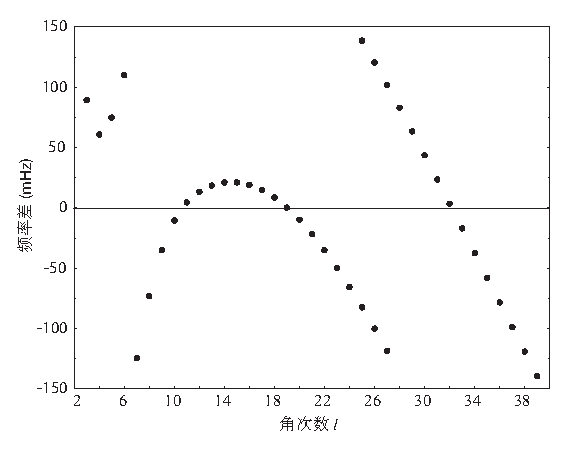
\includegraphics{../figures/chap14/fig19.eps}
}
\end{center}
\caption[fundamentalbranches]{\label{fig:14.fundamentalbranches}
\iffalse
Degenerate eigenfrequency differences along the fundamental spheroidal
and toroidal mode branches on the PREM model.  The quantity
plotted is ${}_0\omega_l^{\rm S}-{}_0\omega_{l+1}^{\rm T}$
in the range $l=7\!-\!28$ and ${}_0\omega_l^{\rm S}-{}_0\omega_{l-1}^{\rm T}$
in the ranges $l=3-6$ and $l=25\!-\!39$.  Coriolis coupling
is most pronounced between the quasi-degenerate multiplet
pairs ${}_0{\rm S}_{11}\!-\!{}_0{\rm T}_{12}$,
${}_0{\rm S}_{19}\!-\!{}_0{\rm T}_{20}$
and ${}_0{\rm T}_{31}\!-\!{}_0{\rm S}_{32}$.
\fi
%%%
PREM~模型中沿基阶球型和环型模式分支的简并本征频率差异。绘制的量为~${}_0\omega_l^{\rm S}-{}_0\omega_{l+1}^{\rm T}$($l=7\!-\!28$)和~${}_0\omega_l^{\rm S}-{}_0\omega_{l-1}^{\rm T}$($l=3-6$~和~$l=25\!-\!39$)。准简并多重态对~${}_0{\rm S}_{11}\!-\!{}_0{\rm T}_{12}$、${}_0{\rm S}_{19}\!-\!{}_0{\rm T}_{20}$~和~${}_0{\rm T}_{31}\!-\!{}_0{\rm S}_{32}$~之间的科里奥利耦合最为显著。
%%%
}
\end{figure}
\iffalse
We focus attention now upon a rotating and elliptical, but laterally
homogeneous, Earth model:
\fi
%%%
现在考虑一个有旋、椭球、但横向均匀的地球模型:
%%%
\eq \label{14.bigrotell}
\ssH^{\rm rot+ell}=\ssN-\nu_0\ssI+\ssW+(2\om_0)^{-1}(\ssV^{\rm ell+cen}
-\om_0^2\ssT^{\rm ell}).
\en
\iffalse
Explicit expressions for the matrix elements of the Coriolis
matrix $\ssW$ and the elliptical-plus-centrifugal matrices
$\ssV^{\rm ell+cen}$ and $\ssT^{\rm ell}$ are given in Appendix~D.
Inspection of these matrices reveals two important facts.
First, in the absence of elastic or anelastic lateral
heterogeneity, the order $m$ of the complex spherical harmonic
$Y_{lm}$ remains a good quantum number; that is, only complex
basis singlets $\tilde{\bs}_k$ having the same order $m$ are
coupled by the Earth's rotation and ellipticity.  Second, the coupling
is governed by the following angular-degree {\em selection rules\/}:
\fi
%%%
科里奥利矩阵~$\ssW$、椭球+离心力矩阵~$\ssV^{\rm ell+cen}$~以及~$\ssT^{\rm ell}$~的矩阵元素的显式表达式已在附录~D~中给出。对这些矩阵的考察揭示了两个重要的事实。首先,在不存在弹性或非弹性横向不均匀性的情况下,复数球谐函数~$Y_{lm}$~的级数~$m$~仍然是一个好量子数;也即,只有具有相同级数~$m$~的复数基单态~$\tilde{\bs}_k$~才会因为地球自转和椭率而耦合。其次,耦合受以下角次数选择法则控制:
%%%
\index{selection rules}%
\index{angular selection rules}%
\begin{enumerate}
\item
\iffalse
The Coriolis force gives rise to spheroidal-toroidal coupling
between multiplets that differ by a {\em single\/} angular degree,
i.e., pairs of the form ${}_n{\rm S}_l\!-\!{}_{n'}{\rm T}_{l\pm1}$
and ${}_n{\rm T}_l\!-\!{}_{n'}{\rm S}_{l\pm1}$.
\fi
%%%
科里奥利力导致相差~1~个角次数的多重态之间产生球型--环型耦合,即为~${}_n{\rm S}_l\!-\!{}_{n'}{\rm T}_{l\pm1}$~和~${}_n{\rm T}_l\!-\!{}_{n'}{\rm S}_{l\pm1}$~的成对形式。
%%%
\item
\iffalse
The Earth's ellipticity gives rise to spheroidal-spheroidal
and toroidal-toroidal coupling between multiplets that
differ in angular degree by {\em two\/}, i.e., pairs of the form
${}_n{\rm S}_l\!-\!{}_{n'}{\rm S}_{l\pm2}$ and
${}_n{\rm T}_l\!-\!{}_{n'}{\rm T}_{l\pm2}$.
\fi
%%%
地球椭率导致相差~2~个角次数的多重态之间产生球型--球型和环型--环型耦合,即~${}_n{\rm S}_l\!-\!{}_{n'}{\rm S}_{l\pm2}$~和~${}_n{\rm T}_l\!-\!{}_{n'}{\rm T}_{l\pm2}$~的成对形式。
%%%
\item
\iffalse
Ellipticity gives rise to coupling between toroidal multiplets of the
{\em same\/} angular degree, i.e., pairs of the form
${}_n{\rm T}_l\!-\!{}_{n'}{\rm T}_l$.
There is no rotational toroidal--toroidal coupling.
\fi
%%%
椭率导致具有相同角次数的环型多重态之间产生耦合,即~${}_n{\rm T}_l\!-\!{}_{n'}{\rm T}_l$~的成对形式,且没有自转环型--环型耦合。
%%%
\item
\iffalse
Rotation and ellipticity both give rise to
coupling between spheroidal multiplets of the {\em same\/}
angular degree, i.e., pairs of the form
${}_n{\rm S}_l\!-\!{}_{n'}{\rm S}_l$.
\fi
%%%
自转和椭率均会导致相同角次数的球型多重态之间产生耦合,即~${}_n{\rm S}_l\!-\!{}_{n'}{\rm S}_l$~的成对形式。
%%%
\end{enumerate}
\iffalse
In general, the coupling between two multiplets $k$ and $k'$
is strong only if their degenerate eigenfrequencies
$\nu_k=\om_k+i\gamma_k$ and $\nu_{k'}=\om_{k'}+i\gamma_{k'}$
are reasonably close.
\fi
%%%
一般情况下,只有当两个多重态~$k$~和~$k'$~的简并本征频率~$\nu_k=\om_k+i\gamma_k$~和~$\nu_{k'}=\om_{k'}+i\gamma_{k'}$~相当接近时,它们之间的耦合效应才是强烈的。
%%%

\iffalse
As shown in Figure~\ref{fig:14.fundamentalbranches},
the real eigenfrequencies of the fundamental-mode
multiplet pairs ${}_0{\rm S}_l\!-\!{}_0{\rm T}_{l+1}$
or ${}_0{\rm T}_l\!-\!{}_0{\rm S}_{l+1}$
are roughly coincident within the {\em Coriolis coupling
band\/},
\index{Coriolis coupling band}%
situated between two and four mHz.
We group the spheroidal and toroidal modes
within this frequency band into triplex super-multiplets
${}_{0}{\rm T}_{l-1}\!-\!{}_0{\rm S}_l\!-\!{}_{0}{\rm T}_{l+1}$ and 
${}_{0}{\rm S}_{l-1}\!-\!{}_0{\rm T}_l\!-\!{}_{0}{\rm S}_{l+1}$,
and diagonalize the $3(2l+1)\times 3(2l+1)$
matrices~(\ref{14.bigrotell}) to find the
split singlet eigenfrequency perturbations
$\delta\nu_j=\delta\om_j+i\,\delta\gamma_j$
and associated eigenvectors $\ssz_j$ and
dual eigenvectors $\overline{\ssz}_j$.
The reference frequency $\nu_0$ for each
triplet is taken to be the degenerate
eigenfrequency of the central or {\em target\/} 
multiplet.
\index{multiplet!target}%
\index{target multiplet}%
The spheroidal-toroidal coupling is particularly
strong between the nearly degenerate
``crossover'' pairs ${}_0{\rm S}_{11}\!-\!{}_0{\rm T}_{12}$,
${}_0{\rm S}_{19}\!-\!{}_0{\rm T}_{20}$
and ${}_0{\rm T}_{31}\!-\!{}_0{\rm S}_{32}$; their singlet eigenfrequencies
are intimately intermingled, and the associated
eigenfunctions and dual eigenfunctions exhibit
roughly equal spheroidal and toroidal characteristics. 
The other quasi-degenerate pairs within
the band are coupled less strongly; their singlet
eigenfrequencies are grouped into recognizable
{\em hybrid multiplets\/}
\index{multiplet!hybrid}%
\index{hybrid multiplet}%
that are either
predominantly spheroidal or predominantly toroidal.
\fi
%%%
如图~\ref{fig:14.fundamentalbranches}~所示,基阶模式多重态对~${}_0{\rm S}_l\!-\!{}_0{\rm T}_{l+1}$~或~${}_0{\rm T}_l\!-\!{}_0{\rm S}_{l+1}$~的实数本征频率在科里奥利耦合频段(即2 ~ 4 mhz)内基本一致。将该频段内的球型和环型模式组合为三重超级多态模式~${}_{0}{\rm T}_{l-1}\!-\!{}_0{\rm S}_l\!-\!{}_{0}{\rm T}_{l+1}$~和~${}_{0}{\rm S}_{l-1}\!-\!{}_0{\rm T}_l\!-\!{}_{0}{\rm S}_{l+1}$,并对角化该~$3(2l+1)\times 3(2l+1)$~维矩阵~(\ref{14.bigrotell})~式,以寻找分裂单态本征频率微扰~$\delta\nu_j=\delta\om_j+i\,\delta\gamma_j$~以及相应的本征向量~$\ssz_j$~和对偶本征向量~$\overline{\ssz}_j$。每个三重态的参考频率~$\nu_0$~被取为是中心或目标多重态的简并本征频率。近乎简并的“交叉”对~${}_0{\rm S}_{11}\!-\!{}_0{\rm T}_{12}$、${}_0{\rm S}_{19}\!-\!{}_0{\rm T}_{20}$~和~${}_0{\rm T}_{31}\!-\!{}_0{\rm S}_{32}$~之间的球型—环型耦合尤其强烈;它们的单态本征频率紧密交织在一起,相应的本征函数和对偶本征函数表现出大致相同的球型和环型特征。该频段内的其他准简并对则耦合较弱;它们的单态本征频率被组合成可识别的混合多重态,并呈现出显著的球型或环型特征。
%%%

\iffalse
In Figure~\ref{fig:14.repell} we plot the {\em mean\/}
real eigenfrequency perturbations
\fi
%%%
在图~\ref{fig:14.repell}~中,我们绘制了相对于次数~$l$~的混合目标模式~${}_0{\rm S}_l$~和~${}_0{\rm T}_l$~的平均实数本征频率微扰,即
%%%
\index{eigenfrequency!mean}%
\index{mean eigenfrequency}%
\eq \label{14.shiftdef}
\langle\delta\om_0\rangle=\frac{1}{2l+1}\sum_j\delta\om_j
\en
\iffalse
of the hybrid target modes ${}_0{\rm S}_l$ and ${}_0{\rm T}_l$
versus degree $l$.  The net effect of Coriolis coupling is
always to shift the centroids $\om_0+\langle\delta\om_0\rangle$
of the quasi-degenerate pairs
${}_0{\rm S}_{l}\!-\!{}_0{\rm T}_{l+1}$ 
or ${}_0{\rm T}_{l}\!-\!{}_0{\rm S}_{l+1}$
away from each other.
This {\em repulsion\/} of the mean eigenfrequencies is
\index{repulsion}%
apparent in the spherical-Earth multiplet strips displayed
in Figures~\ref{fig:10.22} and~\ref{fig:10.23}.
The results in Figure~\ref{fig:14.repell} enable the measured strip
frequencies to be corrected for Coriolis repulsion prior to
inverting for the terrestrial monopole (Masters, Park \&
Gilbert \citeyear{masters&al83}). The strongest repulsion
occurs near the ``crossovers'' $l=11\!-\!12$, $l=19\!-\!20$
and $l=31\!-\!32$, leading to the abrupt offsets or ``tears''
in the plots of $\langle\delta\om_0\rangle$ versus degree.
\fi
%%%
科里奥利耦合的净效应总是使准简并对~${}_0{\rm S}_{l}\!-\!{}_0{\rm T}_{l+1}$~或~${}_0{\rm T}_{l}\!-\!{}_0{\rm S}_{l+1}$~的频率中心~$\om_0+\langle\delta\om_0\rangle$~远离它们每一个。这种平均本征频率之间的互斥在图~\ref{fig:10.22}~和~\ref{fig:10.23}~所示的球对称地球多重态谱条带中较为明显。\textcolor{red}{图~\ref{fig:14.repell}~中的结果使测量到的条带频率能够在为地球单极子反转之前对科里奥利斥力进行校正}(Masters, Park \& Gilbert, \citeyear{masters&al83}))。最强互斥发生在~$l=11\!-\!12$、$l=19\!-\!20$~和$l=31\!-\!32$~的“交叉点”附近,从而导致相对次数的~$\langle\delta\om_0\rangle$~绘图中出现突然偏移或“撕裂”。
%%%

\iffalse
The second-order Coriolis splitting result $\langle\delta\om_0\rangle
=\om_0(\lambda+\third k^2\zeta)(\Omega/\om_0)^2$,
obtained in Section~14.2.3, does a tolerable job of
predicting the repulsive monopole correction
for all of the fundamental-mode coupled multiplets
except the quasi-degenerate pairs
${}_0{\rm S}_{11}\!-\!{}_0{\rm T}_{12}$,
${}_0{\rm S}_{19}\!-\!{}_0{\rm T}_{20}$
and ${}_0{\rm T}_{31}\!-\!{}_0{\rm S}_{32}$.
The quadratic dependence
of the second-order singlet eigenfrequency perturbations,
$\delta\om_m=\om_0[m\chi(\Omega/\om_0)+(\lambda+m^2\zeta)
(\Omega/\omega_0)^2]$, $-l\leq m\leq l$,
upon the order $m$ of the complex spherical harmonic
$Y_{lm}$ is an indication that Coriolis coupling can
also mimic the effect of {\em degree-two zonal\/} heterogeneity
$\delta\hspace{-0.1 mm}\kappa_{20}$, $\delta\hspace{-0.2 mm}\mu_{20}$,
$\delta\hspace{-0.2 mm}\rho_{20}$, $\delta\hspace{-0.1 mm}d_{20}$.
The observed splitting coefficients $\sigma_{20}$ of the fundamental
spheroidal and toroidal modes ${}_0{\rm S}_l$ and ${}_0{\rm T}_l$
must be corrected for this effect,
prior to employing them in any three-dimensional inversion.
Smith \& Masters (\citeyear{smith&masters89b}) show that
this correction significantly improves the along-branch
continuity of the measured coefficients, particularly
in the vicinity of the ``crossover'' pairs
${}_0{\rm S}_{11}\!-\!{}_0{\rm T}_{12}$,
${}_0{\rm S}_{19}\!-\!{}_0{\rm T}_{20}$
and ${}_0{\rm T}_{31}\!-\!{}_0{\rm S}_{32}$.
The perturbation expansion~(\ref{14.DS2}) for these modes
is divergent, indicating the need for the more general
quasi-degenerate theory discussed here.
\fi
%%%
除准简并对~${}_0{\rm S}_{11}\!-\!{}_0{\rm T}_{12}$、${}_0{\rm S}_{19}\!-\!{}_0{\rm T}_{20}$~和~${}_0{\rm T}_{31}\!-\!{}_0{\rm S}_{32}$~外,14.2.3~节中获得的二阶科里奥利分裂结果~$\langle\delta\om_0\rangle
=\om_0(\lambda+\third k^2\zeta)(\Omega/\om_0)^2$~对所有基阶模式耦合多重态的排斥单极子改正均有较好的预测效果。二阶单态本征频率微扰~$\delta\om_m=\om_0[m\chi(\Omega/\om_0)+(\lambda+m^2\zeta)
(\Omega/\omega_0)^2]$, $-l\leq m\leq l$~对~$m$~级复数球谐函数~$Y_{lm}$~的二次依赖性表明,科里奥利耦合也可以模拟二阶带状横向不均匀性~$\delta\hspace{-0.1 mm}\kappa_{20}$、$\delta\hspace{-0.2 mm}\mu_{20}$、$\delta\hspace{-0.2 mm}\rho_{20}$、$\delta\hspace{-0.1 mm}d_{20}$~的影响。基阶球型模式~${}_0{\rm S}_l$~和环型模式~${}_0{\rm T}_l$~的实测分裂系数~$\sigma_{20}$~必须针对这种影响进行修正,然后才能将它们应用于某一~3D~反演。Smith \& Masters~(\citeyear{smith&masters89b})~表明,这种修正可显著改善实测系数的同阶连续性,尤其在“交叉”对~${}_0{\rm S}_{11}\!-\!{}_0{\rm T}_{12}$、${}_0{\rm S}_{19}\!-\!{}_0{\rm T}_{20}$~和~${}_0{\rm T}_{31}\!-\!{}_0{\rm S}_{32}$~附近。这些模式的微扰展开式~(\ref{14.DS2})~是发散的,表明需要对更广义的准简并理论展开讨论。
%%%
\begin{figure}
\begin{center}
\rotatebox{90}
{
\scalebox{0.93}{
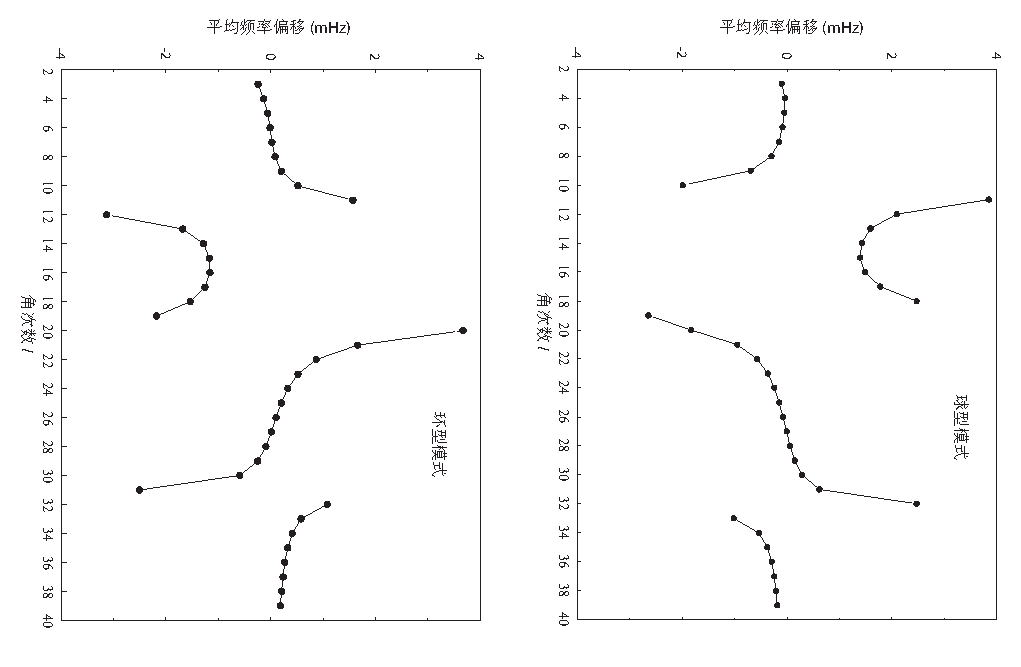
\includegraphics{../figures/chap14/fig20.eps}
}}
\end{center}
\caption[repell]{\label{fig:14.repell}
\iffalse
Mean real eigenfrequency perturbations
$\langle\omega_0\rangle$ of the target
hybrid multiplets ${}_0{\rm S}_l$ ({\em top\/})
and ${}_0{\rm T}_l$ ({\em bottom\/}).
\fi
%%%
目标混合多重态~${}_0{\rm S}_l$(\textcolor{blue}{上图})和~${}_0{\rm T}_l$ (\textcolor{blue}{下图})的平均实数本征频率微~$\langle\omega_0\rangle$
%%%
}
\end{figure}
\begin{figure}
\begin{center}
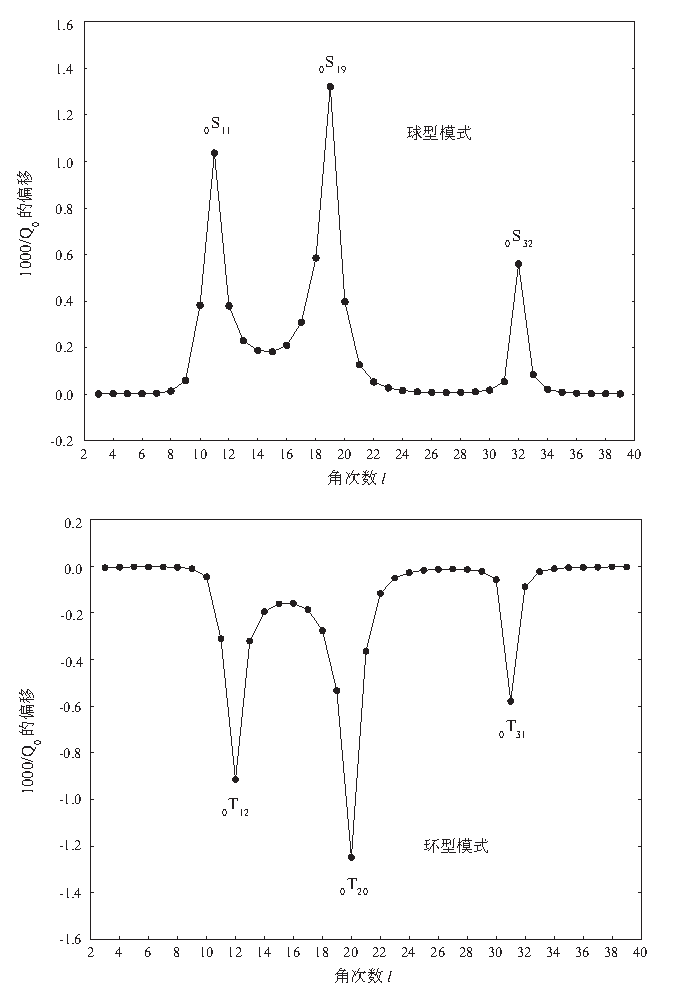
\includegraphics{../figures/chap14/fig21.eps}
\end{center}
\caption[Qshift]{\label{fig:14.Qshift}
\iffalse
Perturbations $1000\,\langle\delta Q_0^{-1}\rangle
=2000\,\omega_0^{-1}\langle\delta\gamma_0\rangle$
in the mean reciprocal quality factors of the
target hybrid multiplets ${}_0{\rm S}_l$
({\em top\/}) and ${}_0{\rm T}_l$ ({\em bottom\/}).
\fi
%%%
目标混合多重态~${}_0{\rm S}_l$~(\textcolor{blue}{上图})和~${}_0{\rm T}_l$~(\textcolor{blue}{下图})的品质因子倒数的平均微扰~$1000\,\langle\delta Q_0^{-1}\rangle
=2000\,\omega_0^{-1}\langle\delta\gamma_0\rangle$
%%%
}
\end{figure}

\iffalse
Each hybrid spheroidal singlet on a rotating, elliptical
Earth experiences a positive decay-rate perturbation,
$\delta\gamma_j>0$, because it has a lower-$Q$
toroidal component, whereas each hybrid toroidal singlet
experiences a negative perturbation, $\delta\gamma_j<0$,
because it it has a higher-$Q$ spheroidal component.
The {\em mean\/} decay rate of each target
\index{decay rate!mean}%
\index{mean decay rate}%
multiplet is therefore shifted by an amount
\fi
%%%
在有旋椭球地球上,每个混合球型单态模式都存在正衰减率微扰,即~$\delta\gamma_j>0$,因为它们有一个较低~$Q$~值的环形分量;而每个混合环型单态模式都存在负衰减率微扰,即~$\delta\gamma_j<0$,因为它们有一个较高~$Q$~值的球型分量。因此,任意目标多重态的平均衰减率偏移量为
%%%
\eq \label{14.shift2}
\langle\delta\gamma_0\rangle=
\frac{1}{2l+1}\sum_j\delta\gamma_j.
\en
\iffalse
This is illustrated in Figure~\ref{fig:14.Qshift},
where we plot the dimensionless shifts $\langle\delta Q_0^{-1}
\rangle=2\om_0^{-1}\langle\delta\gamma_0\rangle$ in
the reciprocal quality factor $Q_0^{-1}$.  Note that the
decay-rate and reciprocal quality-factor centroids
are {\em attracted\/}, whereas the eigenfrequency
\index{attraction}%
\index{repulsion}%
centroids are {\em repelled\/}.
\fi
%%%
这已在图~\ref{fig:14.Qshift}~展示,在该图中我们也绘制了品质因子倒数~$Q_0^{-1}$~的无量纲偏移量~$\langle\delta Q_0^{-1}
\rangle=2\om_0^{-1}\langle\delta\gamma_0\rangle$。注意,衰减率和品质因子的中心是吸引的,而本征频率的中心是排斥的。
%%%

\begin{figure}[!b]
\centering
\begin{tabular}{lr}
\begin{tabular}{l}
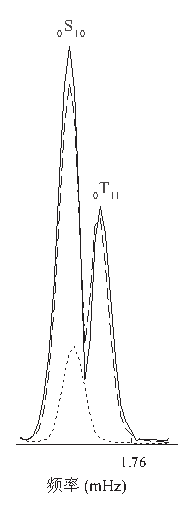
\includegraphics{../figures/chap14/fig22.eps}
\end{tabular}
&
\hspace{0.5cm}
\parbox{5.5cm}{\small
\vspace{0.05cm}
Figure~14.22. 
\iffalse
Radial-component amplitude spectra $|\hat{\bf r}\cdot
{\bf a}({\bf x},\omega)|$ showing the closely spaced hybrid
multiplets ${}_0{\rm S}_{10}$ and ${}_0{\rm T}_{11}$
at station CAN in Canberra, Australia following the
October 4, 1994  Kuril Islands earthquake.  Solid line
shows observed spectrum; dotted line shows synthetic
spectrum for the spherical Earth model PREM; dashed
line shows synthetic spectrum on the rotating, elliptical
version of PREM, with the Coriolis coupling of the modes
${}_{0}{\rm S}_{10}$ and ${}_0{\rm T}_{11}$ accounted for.
\fi
%%%
1994~年~10~月~4~日千岛群岛地震后,澳大利亚堪培拉~CAN~台站的径向分量振幅谱~$|\hat{\bf r}\cdot
{\bf a}({\bf x},\omega)|$~显示处的密集混合多重态~${}_0{\rm S}_{10}$~和~${}_0{\rm T}_{11}$。实线表示观测谱;点线表示球对称地球模型~PREM~的合成谱;虚线表示有旋椭球~PREM~地球模型的合成谱,并考虑了~${}_{0}{\rm S}_{10}$~和~${}_0{\rm T}_{11}$~模式的科里奥利耦合。
%%%
}
\end{tabular}
\end{figure}
\addtocounter{figure}{1}
\iffalse
Coriolis-coupling effects are most pronounced
in the case of a source-receiver path great-circle that
passes over or nearly over the North or South Pole.
A simple physical argument reveals the reason for this
phenomenon.  A fundamental Love wave propagating along
such a polar path has a transverse particle
velocity $\p_t\bs$ that is everywhere perpendicular
to the Earth's angular rotation $\bOmega$;
as a result, it acquires a significant radial
component $\bOmega\times\p_t\bs$ through the
action of the Coriolis force.  The radial
component of a north-south propagating Rayleigh
wave likewise acquires a significant transverse
component; the net result is that the two waves
are strongly coupled by rotation.
Figure~14.22 shows a radial-component
amplitude spectrum $|a(\om)|$ recorded in Canberra,
Australia, nearly due south of the great 1994 Kuril
Islands earthquake.
\index{Kuril Islands 1994 earthquake}%
A peak corresponding to the hybrid
toroidal multiplet ${}_0{\rm T}_{11}$ is clearly visible
on the right shoulder of the peak corresponding to the
hybrid spheroidal mode ${}_0{\rm S}_{10}$.  No such peak
could occur on a non-rotating, spherical Earth, since the
displacement associated with a toroidal mode is purely
tangential.  Coriolis coupling hybridizes the singlets
within the split ${}_0{\rm T}_{11}$ multiplet, and endows
them with an observable radial component; quasi-degenerate
perturbation theory applied to the super-multiplet
${}_{0}{\rm S}_{10}\!-\!{}_0{\rm T}_{11}\!-\!{}_{0}{\rm S}_{12}$
does an excellent job of reproducing the observed spectrum.
\fi
%%%
在震源--接收点路径大圆经过或接近北极或南极点时,科里奥利耦合效应最为显著。一个简单的物理论证即可揭示这种现象的原因。沿着这样一条极路径传播的基阶勒夫波具有一个横向质点速度~$\p_t\bs$,且处处垂直于地球角速度~$\bOmega$;因此,它可以通过科里奥利力作用获得一个显著的径向分量~$\bOmega\times\p_t\bs$。沿南北传播的瑞利波的径向分量同样也获得了一个显著的横向分量;最终结果是这两种波由于地球自转而发生强烈耦合。图~14.22~显示了~1994~年千岛群岛大地震后澳大利亚堪培拉台站(近乎震中的正南方向)记录的径向分量振幅谱~$|a(\om)|$。在混合球型模式~${}_0{\rm S}_{10}$~对应谱峰的右侧,可以看到混合环型多重态~${}_0{\rm T}_{11}$~的对应谱峰。这样的谱峰不可能出现在一个无旋球对称地球上,因为环型模式的相应位移是纯切向的。科里奥利耦合使~${}_0{\rm T}_{11}$~分裂多重态的单态模式杂乱化,并赋予了它们可观测的径向分量;将准简并微扰理论应用于~${}_{0}{\rm S}_{10}\!-\!{}_0{\rm T}_{11}\!-\!{}_{0}{\rm S}_{12}$~超级多态模式,可较好地重构观测谱。
%%%
\index{coupling!rotation|)}%
\index{coupling!ellipticity|)}%

%\subsection{Lateral heterogeneity---selection rules}
\subsection{横向不均匀性--选择法则}
\index{coupling!lateral heterogeneity|(}%

\iffalse
Suppose now that the Earth is laterally heterogeneous,
but neither rotating nor elliptical.  The
$\sum_k(2l_k+1)\,\times\,\sum_k(2l_k+1)$ matrix that
must then be diagonalized is
\fi
%%%
现在假设地球是横向不均匀的,但既无旋也非椭球,那么~$\sum_k(2l_k+1)\,\times\,\sum_k(2l_k+1)$~维矩阵必定是对角化的,即
%%%
\eq \label{14.Hstruct}
\ssH^{\rm lat}=\ssN-\nu_0\ssI+(2\om_0)^{-1}
(\ssV^{\rm lat}-\om_0^2\ssT^{\rm lat}).
\en
\iffalse
In the case that all of the members of the super-multiplet are of the
same type---either spheroidal or toroidal---the
real elements of~(\ref{14.Hstruct}) may be written in a form
analogous to~(\ref{14.Gaunt})--(\ref{eq:14.cst}):
\fi
%%%
若超级多态模式的所有组分都是同一类型(无论是球型还是环型),则~(\ref{14.Hstruct})~式的实数元素可以写成类似~(\ref{14.Gaunt})--(\ref{eq:14.cst})~式的形式:
%%%
\eq \label{eq:14.H}
H_{kk'}^{{\rm lat}\,mm'}=(\om_k-\om_0)+\omega_0\sum_{st}\sigma_{st}^{kk'}
\int_{\Omega}\sY_{lm}\sY_{st}\sY_{l'm'}\,d\Omega,
\en
\iffalse
where
\fi
%%%
其中,
%%%
\eqa
\lefteqn{
\sigma_{st}^{kk'}
=\half\omega_0^{-2}\left(\begin{array}{ccc}
l & s & l' \\
0 & 0 & 0
\end{array}\right)^{-1}
\biggl\{\int_0^a[\delta\hspace{-0.1mm}\kappa_{st}V_\kappa
+\delta\hspace{-0.2mm}\mu_{st}V_\mu
} \nonumber \\
&&\mbox{}
+\delta\hspace{-0.2mm}\rho_{st}(V_\rho-\om_0^2T_\rho)]\,r^2dr
+\sum_d d^2\delta\hspace{-0.1 mm}d_{st}[V_d-\om_0^2T_d]_-^+\biggr\}.
\label{eq:14.cst2}
\ena
\iffalse
Unlike-type (spheroidal-toroidal) coupling is
somewhat more complicated; in that case, the
elements of the complex-basis matrix
$\tilde{\ssH}^{\raisebox{-0.6 ex}{\scriptsize\rm lat}}$
are given in terms of the
expansion coefficients
$\delta\hspace{-0.1mm}\tilde{\kappa}_{st}$,
$\delta\hspace{-0.2mm}\tilde{\mu}_{st}$,
$\delta\hspace{-0.2mm}\tilde{\rho}_{st}$
and $\delta\hspace{-0.1 mm}\tilde{d}_{st}$ by
\fi
%%%
非相同类型(球型--环型)耦合稍微复杂一些;在这种情况下,复数基矩阵~$\tilde{\ssH}^{\raisebox{-0.6 ex}{\scriptsize\rm lat}}$~的元素可由展开系数~$\delta\hspace{-0.1mm}\tilde{\kappa}_{st}$、$\delta\hspace{-0.2mm}\tilde{\mu}_{st}$、$\delta\hspace{-0.2mm}\tilde{\rho}_{st}$~和~$\delta\hspace{-0.1 mm}\tilde{d}_{st}$~给出
%%%
\eq \label{eq:14.Hwiggle}
\tilde{H}_{kk'}^{{\rm lat}\,mm'}=(\om_k-\om_0)+\omega_0\sum_{st}
\tilde{\sigma}_{st}^{kk'}\Gamma_{st}^{kk'},
\en
\iffalse
where
\fi
%%%
其中,
%%%
\eqa
\lefteqn{
\tilde{\sigma}_{st}^{kk'}
=\half\omega_0^{-2}\left(\begin{array}{ccc}
l+1 & s+1 & l'+1 \\
0 & 0 & 0
\end{array}\right)^{-1}
\biggl\{\int_0^a[\delta\hspace{-0.1mm}\tilde{\kappa}_{st}V_\kappa
+\delta\hspace{-0.2mm}\tilde{\mu}_{st}V_\mu
} \nonumber \\
&&\mbox{}
+\delta\hspace{-0.2mm}\tilde{\rho}_{st}(V_\rho-\om_0^2T_\rho)]\,r^2dr
+\sum_d d^2\delta\hspace{-0.1 mm}\tilde{d}_{st}[V_d-\om_0^2T_d]_-^+\biggr\},
\label{eq:14.cst.S-T}
\ena
\eqa \label{14.JTGammadef}
\lefteqn{\Gamma_{st}^{kk'}=(-1)^m
\left[\frac{(2l+1)(2s+1)(2l'+1)}{4\pi}\right]^{1/2}}
\nonumber \\
&&\mbox{}\times
\left(\begin{array}{ccc}
l+1 & s+1 & l'+1 \\
0 & 0 & 0
\end{array}\right)
\left(\begin{array}{ccc}
l & s & l' \\ -m & t & m'
\end{array}\right).
\ena
\iffalse
The associated real elements $H_{kk'}^{{\rm lat}\,mm'}$
may be evaluated using the
complex-to-real transformation
relations~(\ref{D.Ztrans1})--(\ref{D.Ztrans2}).
The order-independent {\em Woodhouse kernels\/}
\index{Woodhouse kernel}%
\index{kernel!Woodhouse}%
$V_\kappa$, $V_\mu$, $V_\rho-\om_0^2T_\rho$,
$V_d-\om_0^2T_d$ in~(\ref{eq:14.cst2})
and~(\ref{eq:14.cst.S-T}) are defined
in equations~(\ref{D.Tsubrho})--(\ref{D.Vsubd}).
\fi
%%%
相应的实数元素~$H_{kk'}^{{\rm lat}\,mm'}$~可利用复数至实数变换关系式~(\ref{D.Ztrans1})--(\ref{D.Ztrans2})~来计算。(\ref{eq:14.cst2})~和~(\ref{eq:14.cst.S-T})~式中的与级数无关的Woodhouse积分核~$V_\kappa$、$V_\mu$、$V_\rho-\om_0^2T_\rho$~和~$V_d-\om_0^2T_d$~被定义在~(\ref{D.Tsubrho})--(\ref{D.Vsubd})~式中。
%%%

\iffalse
Laterally heterogeneous anelasticity may be incorporated
by allowing the perturbed incompressibility and rigidity
to be complex, as in~(\ref{14.alathet}):
\fi
%%%
通过允许扰动的不可压缩性和刚度为复数,横向不均匀非弹性可被靠近进去,如~(\ref{14.alathet})~式所示:
%%%
\eq \label{14.aniHstruct}
\ssH^{\rm lat}=\ssN-\nu_0\ssI+(2\om_0)^{-1}
(\ssV^{\rm lat}+i\ssA-\om_0^2\ssT^{\rm lat}).
\en
\iffalse
The spheroidal-spheroidal and toroidal-toroidal
elements of the anelastic potential energy matrix
$\ssA$ are given by
\fi
%%%
非弹性势能矩阵~$\ssA$~的球型--球型和环型--环型元素为
%%%
\eq
A_{kk'}^{{\rm lat}\,mm'}=\omega_0\sum_{st}\psi_{st}^{kk'}
\int_{\Omega}\sY_{lm}\sY_{st}\sY_{l'm'}\,d\Omega,
\en
\iffalse
where
\fi
%%%
其中,
%%%
\eqa \lefteqn{
\psi_{st}^{kk'}
=\half\omega_0^{-2}\left(\begin{array}{rrr}
l & s & l' \\
0 & 0 & 0
\end{array}\right)^{-1}} \nonumber \\
&&\mbox{}\qquad\qquad\times
\int_0^a(\kappa_0q_{\kappa st}V_\kappa
+\mu_0q_{\mu st}V_\mu)\,r^2dr.
\ena
\iffalse
In the spheroidal-toroidal case, it is again simplest to specify
the elements of the associated complex-basis matrix:
\fi
%%%
在球型--环型情况下,指定相关复数基矩阵的元素同样是最简单的:
%%%
\eq
\tilde{A}_{kk'}^{{\rm lat}\,mm'}=\omega_0\sum_{st}\tilde{\psi}_{st}^{kk'}
\Gamma_{st}^{kk'},
\en
\iffalse
where
\fi
%%%
其中,
%%%
\eqa \lefteqn{
\tilde{\psi}_{st}^{kk'}
=\half\omega_0^{-2}\left(\begin{array}{rrr}
l+1 & s+1 & l'+1 \\
0 & 0 & 0
\end{array}\right)^{-1}} \nonumber \\
&&\mbox{}\qquad\qquad
\times\int_0^a(\kappa_0\tilde{q}_{\kappa st}V_\kappa
+\mu_0\tilde{q}_{\mu st}V_\mu)\,r^2dr.
\ena
\iffalse
The real elements $A_{kk'}^{{\rm lat}\,mm'}$ may
be found, as before, using~(\ref{D.Ztrans1})--(\ref{D.Ztrans2}).
If $\ssA=\sszero$ the splitting matrix~(\ref{14.aniHstruct})
is real and symmetric, whereas if $\ssA\not=\sszero$
it is complex and symmetric.
\fi
%%%
如上所述,利用~(\ref{D.Ztrans1})--(\ref{D.Ztrans2})~式可以确定实数元素~$A_{kk'}^{{\rm lat}\,mm'}$。如果~$\ssA=\sszero$,则分裂矩阵~(\ref{14.aniHstruct})~是实数且对称的;如果~$\ssA\not=\sszero$,则分裂矩阵~(\ref{14.aniHstruct})~是复数且对称的。
%%%

\iffalse
Multiplet-multiplet coupling due to the Earth's
elastic or anelastic lateral heterogeneity is
governed by the following {\em selection rules\/}:
\fi
%%%
由地球弹性或非弹性横向不均匀性引起的多重态--多重态耦合需要遵循如下选择法则:
%%%
\index{selection rules}%
\index{angular selection rules}%
\begin{enumerate}
\item 
\iffalse
A multiplet ${}_n{\rm S}_l$ or ${}_n{\rm T}_l$ is coupled
to a multiplet ${}_{n'}{\rm S}_{l'}$ or ${}_{n'}{\rm T}_{l'}$ by
a lateral variation of degree $s$ only if $|l-l'|\leq s\leq l+l'$.
\fi
%%%
仅当~$|l-l'|\leq s\leq l+l'$~时,多重态~${}_n{\rm S}_l$~或~${}_n{\rm T}_l$~与多重态~${}_{n'}{\rm S}_{l'}$~或~${}_{n'}{\rm T}_{l'}$~因~$s$~阶横向变化而耦合;
%%%
\item 
\iffalse
Two spheroidal multiplets ${}_n{\rm S}_l$ and ${}_{n'}{\rm S}_{l'}$
are coupled by a lateral variation of degree $s$ only if $l+l'+s$ is
{\em even\/}.
\fi
%%%
仅当~$l+l'+s$~为偶数时,两个球型多重态~${}_n{\rm T}_l$~和~${}_{n'}{\rm T}_{l'}$~因~$s$~阶横向变化发生耦合;
%%%
\item 
\iffalse
Two toroidal multiplets ${}_n{\rm T}_l$ and ${}_{n'}{\rm T}_{l'}$
are coupled by a lateral variation of degree $s$ only if $l+l'+s$ is
{\em even\/}.
\fi
%%%
仅当~$l+l'+s$~为偶数时,两个环型多重态~${}_n{\rm T}_l$~和~${}_{n'}{\rm T}_{l'}$~因~$s$~阶横向变化发生耦合;
%%%
\item 
\iffalse
A spheroidal multiplet ${}_n{\rm S}_l$ is coupled to a toroidal
multiplet ${}_{n'}{\rm T}_{l'}$ by a lateral variation of degree $s$
only if $l+l'+s$ is {\em odd\/}.
\fi
%%%
仅当~$l+l'+s$~为奇数时,球型多重态~${}_n{\rm S}_l$~与环型多重态~${}_{n'}{\rm T}_{l'}$~因~$s$~阶横向变化而生耦合。
%%%
\end{enumerate}
\iffalse
The first rule, which governs both like-type and
unlike-type coupling, is simply a restatement of the 3-$j$
triangle condition~(\ref{C.select}).  The next three rules
are an elementary consequence of equation~(\ref{C.mzerod})
and the ``B-factor'' identities~(\ref{D.JHWid1})--(\ref{D.JHWid4}).
\fi
%%%
第一条法同时控制了同类型和不同类型的耦合,是对~3-$j$~三角形条件~(\ref{C.select})~的重申。另外三条法则是~(\ref{C.mzerod})~式“B--因子”恒等式~(\ref{D.JHWid1})--(\ref{D.JHWid4})~的基本结果。
%%%
\index{coupling!lateral heterogeneity|)}%

%\subsection{Generalized diagonal sum rule}
\subsection{广义对角和定则}
\index{diagonal sum rule!generalized|(}%
\index{generalized diagonal sum rule|(}%

\iffalse
The traces of all but the centrifugal-potential matrix
$\ssV^{\rm cen}$ satisfy the diagonal sum rule:
\fi
%%%
除离心势矩阵~$\ssV^{\rm cen}$~外,其他所有复数基矩阵的迹均满足对角和定则:
%%%
\begin{displaymath}
{\rm tr}\,\ssW=0,\qquad{\rm tr}\,\ssT^{\rm ell}=
{\rm tr}\,\ssT^{\rm lat}=0,
\end{displaymath}
\eq \label{14.bigdsum}
{\rm tr}\,\ssV^{\rm ell}={\rm tr}\,\ssV^{\rm lat}=
{\rm tr}\,\ssA=0.
\en
\iffalse
From equation~(\ref{D.diagsum6}) we find that
\fi
%%%
由~(\ref{D.diagsum6})~式可知
%%%
\eq \label{14.bigdsum2}
{\rm tr}\,\ssV^{\rm cen}=\twothirds\Omega^2
\sum_k(2l_k+1)[1-l_k(l_k+1)\chi_k],
\en
\iffalse
where $\chi_k$ is the second-order Coriolis
splitting parameter~(\ref{14.R}) of multiplet
$k$.  The toroidal multiplets ${}_n{\rm T}_l$
do not contribute to the trace~(\ref{14.bigdsum2})
since $1-l_k(l_k+1)\chi_k=0$.  Noting that
${\rm tr}\,(\ssN-\nu_0\ssI)=\sum_k(2l_k+1)(\nu_k-\nu_0)$,
we obtain a super-multiplet generalization
of equations~(\ref{14.dsum3})--(\ref{14.dsum4}):
\fi
%%%
其中,$\chi_k$~是多重态~$k$~的二阶科里奥利分裂参数~(\ref{14.R})。由于~$1-l_k(l_k+1)\chi_k=0$,环型多重态~${}_n{\rm T}_l$~不会对迹~(\ref{14.bigdsum2})~式产生贡献。由于~${\rm tr}\,(\ssN-\nu_0\ssI)=\sum_k(2l_k+1)(\nu_k-\nu_0)$,可得到~(\ref{14.dsum3})--(\ref{14.dsum4})~式的超级多态模式的广义形式:
%%%
\eq \label{14.bigdsum3}
\sum_j\delta\om_j=\sum_{k}(2l_k+1)\Big\{\om_{k}-\om_0
+\twothirds\Omega^2[1-l_k(l_k+1)\chi_k]\Big\},
\en
\eq \label{14.bigdsum4}
\sum_j\delta\gamma_j
=\sum_{k}(2l_k+1)(\gamma_{k}-\gamma_0).
\en
\iffalse
Ignoring the relatively small effect of the spherically
averaged centrifugal potential $\bar{\psi}=-\third\Om^2 r^2$,
the results~(\ref{14.bigdsum3})--(\ref{14.bigdsum4}) stipulate
that the averaged singlet eigenfrequencies and decay rates
of the perturbed Earth model are equal to the corresponding
averages of the terrestrial monopole:
\fi
%%%
忽略球形平均离心势~$\bar{\psi}=-\third\Om^2 r^2$~相对较小的影响,结果式~(\ref{14.bigdsum3})--(\ref{14.bigdsum4})~表明扰动地球模型的平均单态本征频率和衰减率等于相应的地球单极子均值:
%%%
\eq \label{14.D.sum1}
\sum_j(\om_0+\delta\om_j)
=\sum_{k}(2l_k+1)\om_{k},
\en
\eq \label{14.D.sum2}
\sum_j(\gamma_0+\delta\gamma_j)
=\sum_{k}(2l_k+1)\gamma_{k}.
\en
\iffalse
The contributions to the averages~(\ref{14.D.sum1})--(\ref{14.D.sum2})
from each multiplet are weighted by the number $2l_k+1$ of singlets.
This {\em generalized diagonal sum rule\/} is due to
Woodhouse~(\citeyear{woodhouse80}).
\fi
%%%
每个多重态对平均值~(\ref{14.D.sum1})--(\ref{14.D.sum2})~的贡献被单态模式的数量~$2l_k+1$~加权。这种广义对角和定则是由~Woodhouse~~(\citeyear{woodhouse80})~提出的。
%%%
\index{diagonal sum rule!generalized|)}%
\index{generalized diagonal sum rule|)}%

%\subsection{Generalized splitting function}
\subsection{广义分裂函数}
\index{splitting function!generalized|(}%
\index{generalized splitting function|(}%

\iffalse
If we ignore lateral variations in anelasticity and eigenfunction
renormalization, the spectral response~(\ref{14.repeat3}) is given
by the analogue of equation~(\ref{14.myaom}):
\fi
%%%
若忽略非弹性的横向变化和本征函数的重归一化,则频谱响应~(\ref{14.repeat3})~可由~(\ref{14.myaom})~式的类似形式给出:
%%%
\eq \label{14.bigmyaom}
a(\omega)=\half i\ssr^{\rm T}
[\ssH-(\omega-\omega_0-i\gamma_0)\ssI]^{-1}\sss,
\en
\iffalse
where $\ssH=\ssW+(2\om_0)^{-1}[\ssV^{\rm ell+cen}+
\ssV^{\rm lat}-\om_0^2(\ssT^{\rm ell}+\ssT^{\rm lat})]$.
In this approximation, the spectrum of a super-multiplet
depends only upon the characteristics of the source $\bM$, $\bx_{\rm s}$
and receiver $\bnuh$, $\bx$, the known rotation rate
$\Omega$ and hydrostatic ellipticity $\eps(r)$ of the
Earth, and the unknown coefficients $\sigma_{st}^{kk'}$
and $\tilde{\sigma}_{st}^{kk'}$ defined in~(\ref{eq:14.cst2})
and~(\ref{eq:14.cst.S-T}).  By analogy with 
equation~(\ref{eq:14.splittingfunction}), it is customary to define
the {\em generalized splitting function\/}
$\sigma^{kk'}(\theta,\phi)$ of two
coupled multiplets $k$ and $k'$ by
\fi
%%%
其中,$\ssH=\ssW+(2\om_0)^{-1}[\ssV^{\rm ell+cen}+
\ssV^{\rm lat}-\om_0^2(\ssT^{\rm ell}+\ssT^{\rm lat})]$。在这种近似下,某一超级多态模式的频谱只取决于震源~$\bM$~和~$\bx_{\rm s}$、接受点~$\bnuh$~和~$\bx$、已知的地球自转速率~$\Omega$、流体静力学椭率~$\eps(r)$~以及一些由~(\ref{eq:14.cst2})~和~(\ref{eq:14.cst.S-T})~式定义的未知系数~$\sigma_{st}^{kk'}$~和~$\tilde{\sigma}_{st}^{kk'}$。根据~(\ref{eq:14.splittingfunction})~式类推,通常将两个耦合多重态~$k$~和~$k'$~的广义分裂函数~$\sigma^{kk'}(\theta,\phi)$~定义为
%%%
\eq
\sigma^{kk'}=\sum_{s=|l-l'|}^{l+l'}\,
\sum_{t=-s}^s\sigma_{st}^{kk'}\sY_{st}
=\sum_{s=|l-l'|}^{l+l'}\,
\sum_{t=-s}^s\tilde{\sigma}_{st}^{kk'}Y_{st}.
\label{eq:14.generalizedsplittingfunction}
\en
\iffalse
This function of geographical position characterizes
the coupling between two quasi-degenerate multiplets
$k,k'$ in the same manner that the splitting function
$\sigma$ characterizes the self coupling
of a single isolated degenerate multiplet; in the case $k=k'$
the generalized and ordinary splitting functions coincide.
\fi
%%%
该地理位置分布函数描述了两个准简并多重态~$k,k'$~之间的耦合,正如分裂函数~$\sigma$~描述了单个孤立简并多重态的自耦合一样;当~$k=k'$~时,广义分裂函数与普通分裂函数一致。
%%%
\begin{figure}[!t]
\begin{center}
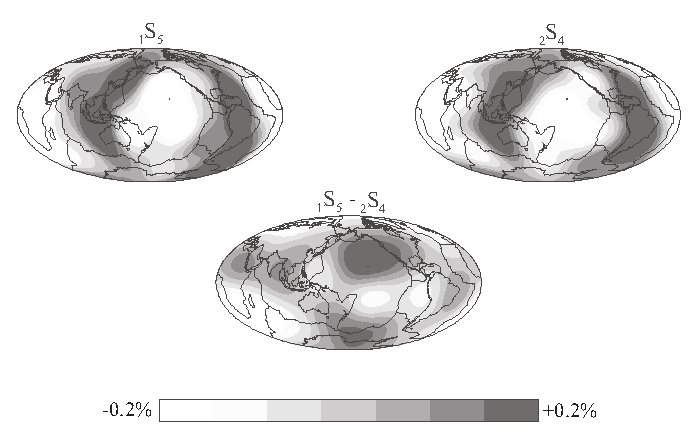
\includegraphics{../figures/chap14/fig23.eps}
\end{center}
\caption[gensplit]{\label{fig:14.gensplit}
\iffalse
Observed generalized splitting functions for the quasi-degenerate
multiplet pair
${}_1{\rm S}_5\!-\!{}_2{\rm S}_4$. ({\em Top left}) \vspace{-0.4 mm}
Function $\sigma^{kk}$ for the mode ${}_1{\rm S}_5$. ({\em Top right})
Function $\sigma^{k'k'}$ for the mode ${}_2{\rm S}_4$.
({\em Bottom}) Function $\sigma^{kk'}\!,k\not=k'$,
governing the interaction between the two modes ${}_1{\rm S}_5$
and ${}_2{\rm S}_4$.  All of the splitting functions have been truncated
in the spectral-fitting process, so that
$\sigma^{kk}$, $\sigma^{k'k'}$ incorporate
only the three even degrees $s=2,4,6$ and $\sigma^{kk'}\!,k\not=k'$,
incorporates only the three odd degrees $s=1,3,5$.
(Courtesy of J. Resovsky \& M. Ritzwoller.)
\fi
%%%
准简并多重态对~${}_1{\rm S}_5\!-\!{}_2{\rm S}_4$~的观测广义分裂函数。(左上图)模式~${}_1{\rm S}_5$~的函数~$\sigma^{kk}$。(右上图)模式~${}_2{\rm S}_4$~的函数~$\sigma^{k'k'}$。(下图)控制模式~${}_1{\rm S}_5$~和~${}_2{\rm S}_4$~之间相互作用的函数~$\sigma^{kk'}\!,k\not=k'$。在频谱拟合过程中,所有的分裂函数都被截断,因此~$\sigma^{kk}$, $\sigma^{k'k'}$~只包含三个偶数阶~$s=2,4,6$,而~$\sigma^{kk'}\!,k\not=k'$~只包含三个奇数阶~$s=1,3,5$。(由~J. Resovsky \& M. Ritzwoller~提供)
%%%
}
\end{figure}
\iffalse
Resovsky \& Ritzwoller
(\citeyear{resovsky&ritzwoller95}; \citeyear{resovsky&ritzwoller98})
have developed and implemented a generalized spectral fitting procedure which first solves for the coefficients $\sigma_{st}^{kk'}$
by minimizing the misfit between a suite of observed and synthetic
super-multiplet spectra $a_p(\om)$, $p=1,2,\ldots$.  \vspace{-0.5 mm}
The measured coefficients $\sigma^{kk'}_{st}$
of a number of super-multiplets may then be used as linear
constraints in a subsequent inversion
for the three-dimensional elastic lateral heterogeneity
$\delta\hspace{-0.1 mm}\kappa_{st}$, $\delta\hspace{-0.2 mm}\mu_{st}$,
$\delta\hspace{-0.2 mm}\rho_{st}$, $\delta\hspace{-0.1 mm}d_{st}$.
In order to describe the splitting and coupling of a cluster
of $K$ multiplets completely, it is necessary to solve for a
total of $\half K(K+1)$ generalized splitting functions.\vspace{-0.5 mm}
\fi
%%%
Resovsky \& Ritzwoller~(\citeyear{resovsky&ritzwoller95}; \citeyear{resovsky&ritzwoller98})~开发并实施了一种广义频谱拟合程序,该程序首先利用一组超级多态模式观测谱与合成谱~$a_p(\om)$, $p=1,2,\ldots$.  \vspace{-0.5 mm}~的偏差最小化来解算系数~$\sigma_{st}^{kk'}$;然后在接下来的反演中,利用一系列超级多态模式的观测系数~$\sigma^{kk'}_{st}$~对三维弹性横向不均匀性参数~$\delta\hspace{-0.1 mm}\kappa_{st}$、$\delta\hspace{-0.2 mm}\mu_{st}$、$\delta\hspace{-0.2 mm}\rho_{st}$~和~$\delta\hspace{-0.1 mm}d_{st}$~进行线性约束。为了完整描述一个多重态簇(包含~$K$~个多重态),总共需要求解~$\half K(K+1)$~个广义分裂函数。
%%%
\begin{sidewaysfigure}
\begin{center}
\rotatebox{270}
{
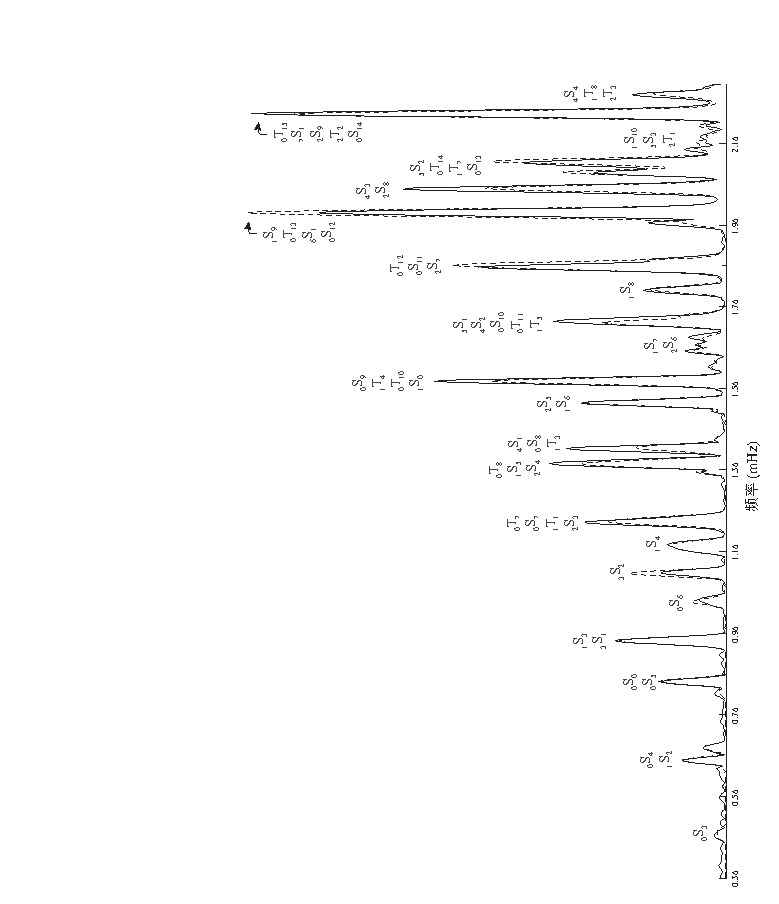
\includegraphics{../figures/chap14/fig24.eps}
}
\end{center}
\caption[pas_spec]{
\iffalse
Radial-component amplitude spectra
%$|\hat{\bf r}\cdot{\bf a}({\bf x},\omega)|$
of the June 9, 1994 Bolivia
deep-focus earthquake recorded at station PAS in
Pasadena, California.  Solid line shows observed
spectrum; dashed line shows synthetic coupled-mode
spectrum.  Rotation, ellipticity and the lateral variations
in shear-wave speed $\delta\hspace{-0.2 mm}\beta$ of model
SKS12WM13 have been accounted for in the calculations.
The vertical arrays of mode labels identify the twenty-two
super-multiplets considered.  A Hann taper has been applied
to both 35-hour time series prior to Fourier transformation.
\fi
%%%
1994~年~6~月~9~日玻利维亚深源地震后,加利福尼亚州帕萨迪纳~PAS~台站记录的径向分量振幅谱。实线表示观测谱,虚线表示合成耦合模式谱。地球自转、椭率以及~SKS12WM13~模型剪切波速度~$\delta\hspace{-0.2 mm}\beta$~的横向变化被考虑到计算中。竖直排列的模式标记确定了所考虑的~22~个超级多态模式。在傅里叶变换之前,对两个~35~小时时间序列均加汉宁窗。
%%%
}
\label{fig:14.pas_spec}
\end{sidewaysfigure}
\begin{sidewaysfigure}
\begin{center}
\rotatebox{270}
{
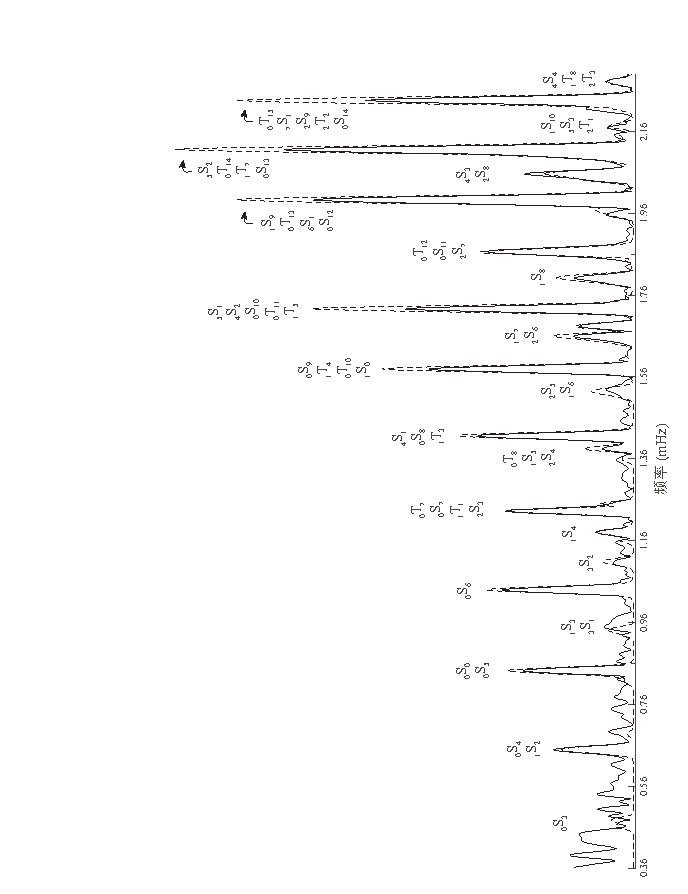
\includegraphics{../figures/chap14/fig25.eps}
}
\end{center}
\caption[ptga_spec]{
\iffalse
Radial-component amplitude spectra
%$|\hat{\bf r}\cdot{\bf a}({\bf x},\omega)|$
of the February 17, 1996 Irian
Jaya earthquake recorded at station PTGA in Pitinga,
Brazil.   Solid line shows observed
spectrum; dashed line shows synthetic coupled-mode
spectrum.  Rotation, ellipticity and the lateral variations
in shear-wave speed $\delta\hspace{-0.2 mm}\beta$ of model
SKS12WM13 have been accounted for in the calculations.
The vertical arrays of mode labels identify the twenty-two
super-multiplets considered.  A Hann taper has been applied
to both 35-hour time series prior to Fourier transformation.
\fi
%%%
1996~年~2~月~17~日巴西伊里安查亚地震后,皮廷加~PTGA~台站记录的径向分量振幅谱。实现表示观测谱,虚线表示合成耦合模式谱。地球自转、椭率以及~SKS12WM13~模型剪切波速度的横向变化~$\delta\hspace{-0.2 mm}\beta$~被考虑到计算中。竖直排列的模式标记确定了所考虑的~22~个超级多态模式。在傅里叶变换之前,对两个~35~小时时间序列均加汉宁窗。
%%%
}
\label{fig:14.ptga_spec}
\end{sidewaysfigure}
\iffalse
Figure~\ref{fig:14.gensplit} shows the three
observed functions $\sigma^{kk}$, $\sigma^{k'k'}$
and $\sigma^{kk'},k\not=k'$ for the $K=2$
super-multiplet ${}_1{\rm S}_5\!-\!{}_2{\rm S}_4$. 
The selection rules in this case of two {\em like-type
multiplets\/} stipulate that both $\sigma_{st}^{kk}$
and $\sigma_{st}^{k'k'}$ are zero whenever $s$ is {\em even\/},
whereas $\sigma_{st}^{kk'}\!,k\not=k'$ is zero whenever
$s$ is {\em odd\/}.  Spectra of ${}_1{\rm S}_5\!-\!{}_2{\rm S}_4$
are sensitive to {\em both\/} the even-degree and odd-degree
heterogeneity in the range $1\leq s\leq 10$.  A total of 164
generalized splitting coefficients must
be measured in order to account for this sensitivity fully.
\fi
%%%
图~\ref{fig:14.gensplit}~给出了超级多态模式~${}_1{\rm S}_5\!-\!{}_2{\rm S}_4$($K=2$)的三个观测函数~$\sigma^{kk}$、$\sigma^{k'k'}$~和~$\sigma^{kk'},k\not=k'$。在两个同类型多重态情况下,选择法则规定,当~$s$~为偶数时,$\sigma_{st}^{kk}$~和~$\sigma_{st}^{k'k'}$~均为零;而当~$s$~为奇数时,$\sigma_{st}^{kk'}\!,k\not=k'$~为零。${}_1{\rm S}_5\!-\!{}_2{\rm S}_4$~的频谱对~$1\leq s\leq 10$~范围内的偶数阶和奇数阶不均匀性都较为敏感。为充分解释这种敏感性,总共必须测量~164~个广义分裂系数。
%%%
\index{splitting function!generalized|)}%
\index{generalized splitting function|)}%

%\subsection{Whole-spectrum fitting}
\subsection{全频谱拟合}
\index{whole-spectrum fitting|(}%
\index{spectral fitting|(}%

\iffalse
At higher frequencies, the spectrum becomes denser and
grouping modes into identifiable super-multiplets becomes
more difficult.  In addition, the number of singlets
within each ``isolated'' super-multiplet increases.
\fi
%%%
在较高频率处,频谱变得更密集,将模式分组为可识别的超级多态模式变得更困难。
%%%
\begin{figure}[!t]
\begin{center}
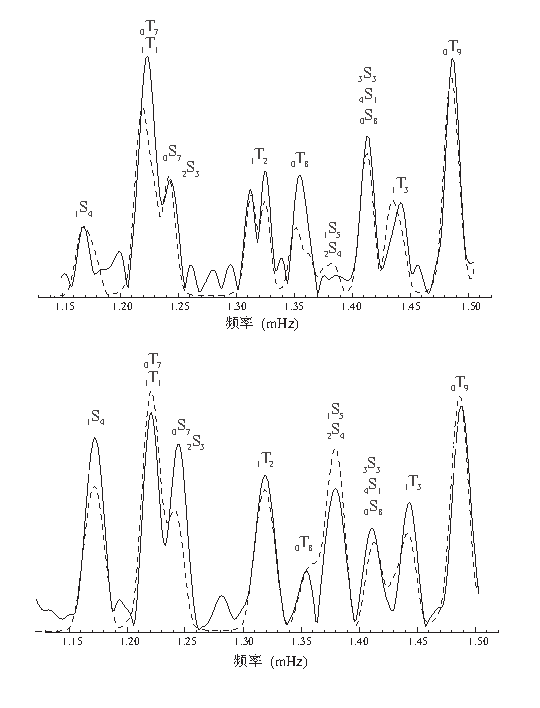
\includegraphics{../figures/chap14/fig26.eps}
\end{center}
\caption[trans_specs]{\label{fig:14.trans_specs}
\iffalse
Amplitude spectra $|\hat{\bf \Phi}\cdot{\bf a}({\bf x},\omega)|$
of the June 9, 1994 Bolivia deep-focus earthquake recorded
on the transverse components at stations ANMO in
Albuquerque, New Mexico ({\em  top}) and PAB
in San Pablo, Spain ({\em  bottom}).   Solid lines show
observed spectra; dashed lines show synthetic coupled-mode
spectra.  Rotation, ellipticity and the lateral variations
in shear-wave speed $\delta\hspace{-0.2 mm}\beta$ of model
SKS12WM13 have been accounted for in the calculations.
The vertical arrays of mode labels identify the
super-multiplets considered.  A Hann taper has been applied
to all four 45-hour time series prior to Fourier transformation.
\fi
%%%
1994~年玻利维亚地震后,新墨西哥州阿尔伯克基~ANMO~台站(上图)和西班牙圣帕布罗~PAB~台站(下图)记录的横向分量振幅谱~$|\hat{\bf \Phi}\cdot{\bf a}({\bf x},\omega)|$。地球自转、椭率以及~SKS12WM13~模型剪切波速度的横向变化~$\delta\hspace{-0.2 mm}\beta$~被考虑到计算中。竖直排列的模式标记确定了所考虑的超级多态模式。在傅里叶变换之前,对四个~45~小时序列均加汉宁窗。
%%%
}
\end{figure}
\iffalse
For these reasons, the determination of generalized
splitting functions rapidly becomes impractical.
Rather than employing the two-step approach described
above, it is preferable to fit whole portions of a
suite of spectra $a_p(\om)$, $p=1,2,\ldots$, in a single-step inversion
for the elastic lateral heterogeneity
$\delta\hspace{-0.1 mm}\kappa_{st}$,
$\delta\hspace{-0.2 mm}\mu_{st}$,
$\delta\hspace{-0.2 mm}\rho{st}$,
$\delta\hspace{-0.1 mm}d_{st}$ of the mantle.
Such {\em whole-spectrum fitting\/} is
eminently feasible, given the power of
contemporary computers and the high quality
of modern digital seismic data.  Current
shear-wave speed models such as SKS12WM13
(Dziewonski, Liu \& Su \citeyear{liu&dziewonski96})
often provide quite acceptable initial fits,
as we illustrate in Figure~\ref{fig:14.pas_spec}.
The solid line shows the radial-component amplitude
spectrum recorded in Pasadena, California, following
the June 9, 1994 deep-focus earthquake in Bolivia;
\index{Bolivia 1994 earthquake}% 
the dashed line shows the corresponding synthetic
spectrum for a rotating, elliptical version of
model SKS12WM13, calculated by grouping all
of the identified modes into super-multiplets identified by
the vertically stacked labels.  It is remarkable how well
this Earth model---which does not incorporate any normal-mode
splitting constraints---fits the observed low-frequency spectrum.
Needless to say, no model---not even the latest and greatest from Harvard---is a seismological panacea; the
fit of SKS12WM13 to a more typical spectrum, recorded in
Pitinga, Brazil following the February 17, 1996 Irian Jaya
earthquake, is shown in Figure~\ref{fig:14.ptga_spec}.
\index{Irian Jaya 1996 earthquake}%
The signal-to-noise ratio is significantly higher in
this example, particularly beneath $1\!-\!1.5$ mHz.
A pair of transverse-component spectra recorded
in Albuquerque, New Mexico and
San Pablo, Spain after the 1994 Bolivia
event are shown in Figure~\ref{fig:14.trans_specs}.
A number of spheroidal modes such as the triplet
${}_3{\rm S}_3\!-\!{}_4{\rm S}_1\!-\!{}_0{\rm S}_8$
are a prominent feature of these spectra.  With a few
exceptions such as the doublet ${}_0{\rm S}_7\!-\!{}_2{\rm S}_3$
at San Pablo, these multiplets are well fit by the SKS12WM13
coupled-mode synthetics.  Note, finally, that the toroidal
multiplet ${}_1{\rm T}_2$ is visibly split at Albuquerque.
\fi
%%%
此外,每个“孤立的”超级多态模式内的单态模式数目会增加。由于这些原因,快速确定广义分裂函数变得不切实际。与其采用上文所述的两步法,不如直接采用单步反演来拟合一组频谱~$a_p(\om)$, $p=1,2,\ldots$~的全部部分,以此研究地幔的弹性横向非均匀性~$\delta\hspace{-0.1 mm}\kappa_{st}$、$\delta\hspace{-0.2 mm}\mu_{st}$、$\delta\hspace{-0.2 mm}\rho{st}$~和~$\delta\hspace{-0.1 mm}d_{st}$。凭借现代计算机的高效计算能力和现代数字地震数据的高质量,这种全频谱拟合是非常可行的。如图~\ref{fig:14.pas_spec}~所示,目前的剪切波速度模型,如~SKS12WM13~(Dziewonski, Liu \& Su  \citeyear{liu&dziewonski96}),经常可提供相当可靠的初始拟合结果。图中实线显示了~1994~年~6~月~9~日玻利维亚深源地震后加利福尼亚州帕萨迪纳台站记录的径向分量振幅谱;虚线表示基于有旋、椭球~SKS12WM13~模型获取的相应合成谱,\textcolor{red}{该合成谱是通过将所有被识别的模式分组到由竖直堆叠标签识别的超级多态模式来计算的}。\textcolor{red}{注意},该地球模型不包含任何简正模式分裂约束,但与低频观测谱较为符合。当然,没有任何模型能完美解决地震学的所有问题,即使是哈佛大学最新最优的模型。图~\ref{fig:14.ptga_spec}~显示了~1996~年~2~月~17~日巴西伊里安查亚地震后~SKS12WM13~模型合成谱与皮廷加台站获取的更典型观测谱的拟合情况。该例中的信号信噪比要高得多,尤其是在~$1\!-\!1.5$~mHz~以下。图~\ref{fig:14.trans_specs}~显示了~1994~年玻利维亚地震后新墨西哥州阿尔伯克基和西班牙圣帕布罗台站记录的一对横向分量谱。大量球型模式,如~${}_3{\rm S}_3\!-\!{}_4{\rm S}_1\!-\!{}_0{\rm S}_8$~三重态,是这些频谱的一个显著特征。在圣帕布罗台站,除~${}_0{\rm S}_7\!-\!{}_2{\rm S}_3$~二重态等少数例外,其他多重态观测谱与~SKS12WM13~耦合模式合成谱符合较好。最后值得注意的是,在阿尔伯克基台站,环型多重态~${}_1{\rm T}_2$~发生明显分裂。
%%%
\index{whole-spectrum fitting|)}%
\index{spectral fitting|)}%

\renewcommand{\thesubsection}{$\!\!\!\raise1.3ex\hbox{$\star$}\!\!$
\arabic{chapter}.\arabic{section}.\arabic{subsection}}
%\subsection{Along-branch coupling}
\subsection{同级耦合}
\index{along-branch coupling|(}%
\index{coupling!along-branch|(}%
\renewcommand{\thesubsection}{\arabic{chapter}.\arabic{section}.\arabic{subsection}}

\iffalse
Cross-branch coupling between surface-wave equivalent modes with
distinct overtone numbers, $n\not= n'$, is weak or absent upon a smooth,
laterally heterogeneous Earth model, by virtue of the triangle selection rule.
In fact, two multiplets ${}_n{\rm S}_l$ or ${}_n{\rm T}_l$,
$n\ll l$, and
${}_{n'}{\rm S}_{l'}$ or ${}_{n'}{\rm T}_{l'}$, $n'\ll l'$, are completely
uncoupled by lateral heterogeneity of maximum angular degree
$s_{\rm max}<|l-l'|$.  This is a strong constraint, particularly
at high frequency, where the surface-wave dispersion branches are
well separated.  At a period $2\pi/\omega\approx 100$~s, the spacing
\fi
%%%
根据三角选择法则,在一个平滑且横向不均匀的地球模型中,具有不同泛音数~$n\not= n'$~的面波等效模式之间的跨支耦合较弱或不存在。事实上,由于最大角阶数~$s_{\rm max}<|l-l'|$~的横向不均匀性,两个多重态~${}_n{\rm S}_l$~或~${}_n{\rm T}_l$($n\ll l$)~和~${}_{n'}{\rm S}_{l'}$~或~${}_{n'}{\rm T}_{l'}$($n'\ll l'$ )是完全解耦的。这是一个强约束条件,尤其是在高频,面波频散分支曲线彼此完全分离。在周期~$2\pi/\omega\approx 100$~s~时,
%%%
\begin{figure}[!b]
\begin{center}
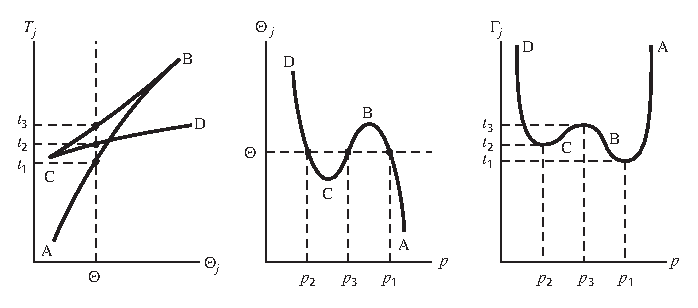
\includegraphics{../figures/chap14/fig27.eps}
\end{center}
\caption[junho1]{\label{14.fig.junho1}
\iffalse
Synthetic radial-component acceleration
spectra $|\hat{\bf r}\cdot{\bf a}({\bf x},\omega)|$
for the ${}_0{\rm S}_{55}$ multiplet at stations
GAR ({\em top\/}) and KIP ({\em bottom\/}), following the 1978 Oaxaca, Mexico
earthquake.  The 111 singlet eigenfrequencies and eigenfunctions have been
calculated by numerical diagonalization of the real symmetric splitting
matrix~(\ref{14.realHst}).  Rotation has been ignored, but the Earth's
hydrostatic ellipticity has been accounted for.
The coupling along the fundamental
spheroidal branch has been truncated at various levels, ranging
from $\pm 0$ ({\em left\/}) to $\pm 8$ ({\em right\/}).
The spectra are calculated using a Hann taper on
records of 20 hr duration.
Dotted curves show the corresponding spectra on a spherically symmetric Earth
for comparison.
\fi
%%%
1978~年墨西哥瓦哈卡地震后,GAR(上图)和~KIP~台站(下图)的~${}_0{\rm S}_{55}$~多重态的合成径向加速度谱~$|\hat{\bf r}\cdot{\bf a}({\bf x},\omega)|$。通过实数对称分裂矩阵~(\ref{14.realHst})~的数值对角化,计算了~111~个单态模式的本征频率和本征函数。地球自转被忽略,但考虑了流体静力学椭率。沿基阶球型分支的耦合在不同阶数上被截断,范围为~$\pm 0$~至~$\pm 8$~(从左至右)。对~20~小时持续记录加汉宁窗以计算频谱。为作比较,用点线表示球对称地球的相应频谱。
%%%
}
\end{figure}
\iffalse
between the fundamental and first-overtone toroidal modes
${}_0{\rm T}_l$, ${}_1{\rm T}_{l'}$ is $|l-l'|\approx 20$,
whereas that between the fundamental and first-overtone spheroidal
modes ${}_0{\rm S}_l$, ${}_1{\rm S}_{l'}$ is $|l-l'|\approx 30$
(see Figures~\ref{fig:tormodefreqs} and~\ref{fig:sphmodefreqs}).
Because of this circumstance, it is common to ignore cross-branch
coupling when synthesizing surface-wave seismograms on a non-rotating Earth
by means of normal-mode summation.  Spheroidal-toroidal coupling
is also negligible between surface-wave equivalent multiplets
${}_n{\rm S}_l$, $n\ll l$, and ${}_{n'}{\rm T}_{l'}$, $n'\ll l'$,
as we shall see in Chapter~16. The only structural coupling which
must be accounted for on a smooth isotropic
\fi
%%%
基阶和一阶环型模式~${}_0{\rm T}_l$, ${}_1{\rm T}_{l'}$~之间的间隔为~$|l-l'|\approx 20$,而基阶和一阶球型模式~${}_0{\rm S}_l$、${}_1{\rm S}_{l'}$~之间的间隔为~$|l-l'|\approx 30$(见图~\ref{fig:tormodefreqs}~和~\ref{fig:sphmodefreqs}))。在这种情况下,采用简正模求和方法合成无旋地球的面波地震图时,常常忽略跨支耦合。面波等效多重态~${}_n{\rm S}_l$($n\ll l$)和~${}_{n'}{\rm T}_{l'}$ ($n'\ll l'$)之间的球型--环型耦合同样被忽略(见第~16~章)。
%%%
\begin{figure}[!t]
\begin{center}
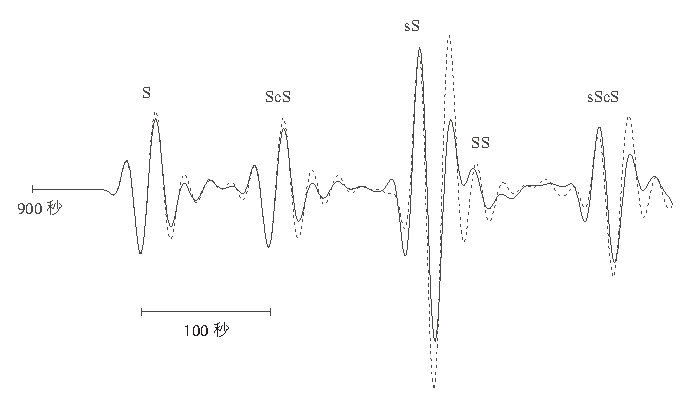
\includegraphics{../figures/chap14/fig28.eps}
\end{center}
\caption[junho2]{\label{14.fig.junho2}
\iffalse
Instantaneous amplitude ({\em top\/}) and phase ({\em bottom\/})
of the normalized multiplet modulation function $A_0(t)/A_0$
of mode ${}_0{\rm S}_{35}$ at station GAR following the 1978
Oaxaca earthquake.  The radial acceleration is given
in terms of $A_0(t)$ by $\hat{\bf r}\cdot{\bf a}
({\bf x},t)={\rm Re}\,[A_0(t)\exp(i\omega_0t-\gamma_0t)]$.
All of the modulation functions are calculated using an
along-branch coupling scheme, with various levels of
truncation: $\pm 0$ ({\em dotted line\/}), $\pm 1$
({\em dot-dash line\/}), $\pm 5$ ({\em dashed line\/})
and $\pm s_{\rm max}=\pm 8$ ({\em solid line\/}).
In the $\pm 0$ or self-coupling approximation,
the initial value of the normalized modulation
function is $A_0(0)/A_0=1$, as shown.
\fi
%%%
1978~年瓦哈卡地震后,GAR~台站~${}_0{\rm S}_{35}$~模式的归一化多重态调制函数~$A_0(t)/A_0$~的瞬时振幅(上图)和相位(下图)。径向加速度由~$A_0(t)$ 以 $\hat{\bf r}\cdot{\bf a}
({\bf x},t)={\rm Re}\,[A_0(t)\exp(i\omega_0t-\gamma_0t)]$~的形式给出。所有调制函数均采用同级耦合方案计算,截断阶数分别为~$\pm 0$(点线)、$\pm 1$(点虚线)、$\pm 5$(虚线)和~$\pm s_{\rm max}=\pm 8$(实线)。如图所示,在~$\pm 0$~或自耦合近似下,归一化调制函数的初始值为~$A_0(0)/A_0=1$。
%%%
}
\end{figure}
\iffalse
Earth model is that along the individual dispersion
branches $\cdots{}_n{\rm S}_{l-1}\!-\!{}_n{\rm S}_l\!-\!
{}_n{\rm S}_{l+1}\cdots$ and $\cdots{}_n{\rm T}_{l-1}\!-\!{}_n{\rm T}_l\!-\!
{}_n{\rm T}_{l+1}\cdots$.  The shifting-and-winnowing procedure
described in Section~\ref{13.sec.hybrid} can be used to compute
a ``seamless'' single-branch accelerogram; each target multiplet
${}_n{\rm S}_l$ or ${}_n{\rm T}_l$ is coupled to its nearest
$\pm L$ neighbors ${}_n{\rm S}_{l\pm 1},{}_n{\rm S}_{l\pm 2},
\ldots,{}_n{\rm S}_{l\pm L}$ or ${}_n{\rm T}_{l\pm 1},{}_n{\rm T}_{l\pm 2},
\ldots,{}_n{\rm T}_{l\pm L}$.  This is referred to as $\pm L$ coupling.
The method is profligate, inasmuch as $(2L+1)(2l+1)$ eigenvalues and
eigenvectors must be computed for each target, and only $2l+1$ of
these are retained.  On an Earth model with spherically symmetric
attenuation, $\ssA=\sszero$, it is possible to reduce the computational
burden by ignoring the slight variation in the spherical-Earth decay
rate along a dispersion branch.  Upon making the approximation
$\gamma_k=\gamma_0$ in equation~(\ref{14.Hstruct}) we obtain
a {\em real\/} symmetric splitting matrix
\fi
%%%
在平滑且各向同性的地球模型中,沿着单个频散分支~$\cdots{}_n{\rm S}_{l-1}\!-\!{}_n{\rm S}_l\!-\!
{}_n{\rm S}_{l+1}\cdots$~和~$\cdots{}_n{\rm T}_{l-1}\!-\!{}_n{\rm T}_l\!-\!
{}_n{\rm T}_{l+1}\cdots$~的耦合是必须考虑的唯一结构耦合。第~\ref{13.sec.hybrid}~节中描述的偏移和筛选过程可用于计算“无缝”单分支加速度图;每个目标多重态~${}_n{\rm S}_l$~或~${}_n{\rm T}_l$~会与其最临近的~$\pm L$~多重态~${}_n{\rm S}_{l\pm 1},{}_n{\rm S}_{l\pm 2},
\ldots,{}_n{\rm S}_{l\pm L}$~或~${}_n{\rm T}_{l\pm 1},{}_n{\rm T}_{l\pm 2},
\ldots,{}_n{\rm T}_{l\pm L}$~发生耦合。这种耦合被称为~$\pm L$~耦合。由于对每个目标必须计算~$(2L+1)(2l+1)$~个特征值和特征向量,但只保留了其中~$2l+1$~个,因此该方法\textcolor{red}{存在计算冗余}。在球对称衰减的地球模型中,$\ssA=\sszero$,可通过忽略沿频散分支的球对称地球衰减率的微小变化来减轻计算负担。通过对式~(\ref{14.Hstruct})~采用~$\gamma_k=\gamma_0$~近似,可得到了一个实数对称分裂矩阵
%%%
\eq \label{14.realHst}
\ssH^{\rm lat}=\ssOmega-\om_0\ssI+(2\om_0)^{-1}
(\ssV^{\rm lat}-\om_0^2\ssT^{\rm lat}),
\en
\iffalse
where $\ssOmega={\rm diag}\,[\,\cdots\om_k\cdots\,]$
is the diagonal matrix of degenerate eigenfrequencies.
At high frequencies and on rough Earth models,
the split singlets of adjacent along-branch multiplets can overlap,
and the ranking and winnowing of the eigenvalues
$\delta\omega_j$ fails.
\fi
%%%
其中,$\ssOmega={\rm diag}\,[\,\cdots\om_k\cdots\,]$~是简并本征频率的对角化矩阵。在高频段和粗糙地球模型上,相邻的同级多重态的分裂单态模式会发生重叠,导致特征值~$\delta\omega_j$~的排序和筛选失效。
%%%

\begin{figure}[!b]
\begin{center}
\includegraphics{../figures/chap14/fig29.eps}
\end{center}
\caption[junho3]{\label{14.fig.junho3}
\iffalse
Same as Figure~\ref{14.fig.junho2}, except for
the higher-frequency multiplet ${}_0{\rm S}_{55}$.
\fi
%%%
与图~\ref{14.fig.junho2}~相同,但目标模式为更高频多重态~${}_0{\rm S}_{55}$。
%%%
}
\end{figure}
\iffalse
Figure~\ref{14.fig.junho1} shows some representative synthetic
acceleration spectra on the $s_{\rm max}=8$ Earth model M84A
(Woodhouse \& Dziewonski \citeyear{woodhouse&dziewonski84}).
The response of the ${}_0{\rm S}_{55}$ fundamental spheroidal
multiplet ($2\pi/\om=165$~s) to the November 29, 1978
Oaxaca, Mexico earthquake
\index{Oaxaca 1978 earthquake}%
has been computed using
a self-coupling or $\pm0$ as well as a $\pm 1$, $\pm 5$ and
$\pm 8$ coupling scheme; the dashed curve shows the corresponding
spherical-Earth spectrum in each case.  At station GAR in Garm,
Tajikistan the interference of the 111 singlets gives rise to
a somewhat misshapen spectral peak whose overall amplitude
is much less than that on PREM; at station KIP in Kipapa, Hawaii
the amplitude is slightly greater than that on PREM, and there is
a significant shift in the centroid of the ``singlet-like'' peak
toward higher frequency.  In both cases, the results are seen to
converge as the degree of along-branch coupling is increased.
Self-coupling cannot account for the suppressed amplitude at GAR;
however, truncation of the coupling at $\pm 5$ yields virtually
identical results to $\pm s_{\rm max}=\pm 8$.
In Figures~\ref{14.fig.junho2} and~\ref{14.fig.junho3} we
illustrate the ${}_0{\rm S}_{35}$ and ${}_0{\rm S}_{55}$ multiplet
modulation functions; the quantities plotted are the instantaneous
amplitude and phase of the dimensionless ratio $A_0(t)/A_0$,
normalized by the real amplitude $A_0$ on a spherical Earth.
The time scale of the variations is more rapid for ${}_0{\rm S}_{55}$
than for ${}_0{\rm S}_{35}$, and the effect of along-branch truncation is
more significant, as expected.  As in the frequency domain, $\pm 5$
along-branch coupling is seen to be a very good approximation,
on a smooth Earth model such as M84A.\vspace{-0.5mm}
\fi
%%%
图~\ref{14.fig.junho1}~显示了~$s_{\rm max}=8$~阶地球模型~M84A(Woodhouse \& Dziewonski~\citeyear{woodhouse&dziewonski84}))上一些具有代表性的合成加速度谱。采用自耦合(或~$\pm0$)以及~$\pm 1$、$\pm 5$、$\pm 8$~阶耦合方案,计算了~${}_0{\rm S}_{55}$~基阶球型多重态($2\pi/\om=165$~s)对~1978~年~11~月~29~日墨西哥瓦哈卡地震的响应;虚线表示每种情况下相应的球对称地球频谱。在塔吉克斯坦嘉尔姆的~GAR~台站,111~个单态模式的干扰导致谱峰产生轻微畸变,其总体幅值远小于~PREM~模型合成值;在夏威夷~Kipapa~的~KIP~台站,其振幅略大于~PREM~模型合成值,且“似单态”谱峰的中心向高频方向显著偏移。在这两个案例中,随着同级耦合阶次的增加,计算结果趋于收敛。自耦合无法解释~GAR~台站的抑制振幅;然而,在~$\pm 5$~阶处耦合截断计算的结果与~$\pm s_{\rm max}=\pm 8$~处几乎相同。图~\ref{14.fig.junho2}~和~\ref{14.fig.junho3}~展示了~${}_0{\rm S}_{35}$~和~${}_0{\rm S}_{55}$~多重态的调制函数;图中物理量是采用无量纲比 的瞬时振幅和相位,且由球对称地球上的实数振幅 归一化。${}_0{\rm S}_{35}$~变化的时间尺度比~${}_0{\rm S}_{55}$~更快,同级截断的影响更显著。在频率域中,对于平滑地球模型(如~M84A),$\pm 5$~阶同级耦合是一个较优的近似。
%%%

\begin{figure}[!b]
\begin{center}
\includegraphics{../figures/chap14/fig30.eps}
\end{center}
\caption[junho4]{\label{14.fig.junho4}
\iffalse
Synthetic radial-component acceleration
spectra $|\hat{\bf r}\cdot{\bf a}({\bf x},\omega)|$
for the ${}_0{\rm S}_{55}$ multiplet at stations
GAR ({\em top\/}) and KIP ({\em bottom\/}), following the 1978 Oaxaca
earthquake.  Spectra calculated using the Woodhouse-Dziewonski great-circle
approximation ({\em left\/}), the quasi-isolated multiplet approximation
({\em middle\/}) and the full variational method truncated at $\pm 8$
({\em right\/}) are compared.  The triangle selection rule insures that
the lowest-order quasi-isolated multiplet approximation is naturally
truncated at $\pm 8$ on an $s_{\rm max}=8$ Earth model such as M84A.
All spectra are calculated using a Hann taper on records of 20 hr duration.
Dashed curves show the corresponding spherical-Earth
spectra for comparison.
\fi
%%%
1978~年墨西哥瓦哈卡地震后,GAR(上图)和~KIP~台站(下图)${}_0{\rm S}_{55}$~多重态的合成径向加速度谱~$|\hat{\bf r}\cdot{\bf a}({\bf x},\omega)|$。图中比较了采用~Woodhouse--Dziewonski~大圆近似(左图)、准孤立多重态近似(中图)和~$\pm 8$~阶截断的全变分法(右图)计算的频谱。三角选择法则确保了最低阶准孤立多重态近似在~$s_{\rm max}=8$~阶地球模型(如~M84A)上以~$\pm 8$~阶自然截断。对~20~小时持续记录均加汉宁窗以计算频谱。为作比较,用虚线表示球对称地球相应的频谱。
%%%
}
\end{figure}
\iffalse
In Figure~\ref{14.fig.junho4} we use the $\pm 8$ coupled-mode
results at KIP and GAR
as ``ground truth'' to assess the accuracy of two alternative and much
more efficient methods of synthesizing long-period
surface-wave accelerograms:
\fi
%%%
在图~\ref{14.fig.junho4}~中,我们采用~KIP~和~GAR~台站的~$\pm 8$~阶耦合模式结果作为“地表真值”,
%%%
\begin{figure}[!t]
\begin{center}
\includegraphics{../figures/chap14/fig31.eps}
\end{center}
\caption[junho5]{\label{14.fig.junho5}
\iffalse
Instantaneous amplitude ({\em top\/}) and phase ({\em bottom\/})
of the normalized multiplet modulation function $A_0(t)/A_0$
of mode ${}_0{\rm S}_{35}$ at station GAR following the 1978
Oaxaca earthquake.  Temporal variations calculated using the Woodhouse-Dziewonski
great-circle approximation ({\em dotted line\/}), the quasi-isolated
multiplet approximation ({\em dash-dot line\/}) and the $\pm 8$ variational
method ({\em solid line\/}) are compared.
\fi
%%%
1978~年瓦哈卡地震后,GAR~台站~${}_0{\rm S}_{35}$~模式的归一化多重态调制函数~$A_0(t)/A_0$~的瞬时振幅(上图)和相位(下图)。图中比较了采用~Woodhouse--Dziewonski~大圆近似(虚线)、准孤立多重态近似(虚线)和~$\pm 8$~阶截断的全变分法(实线)计算的时域变化。
%%%
}
\end{figure}
\iffalse
the lowest-order quasi-isolated multiplet approximation discussed in
Section~13.3.5, and the path-average or {\em great-circle approximation\/}
\index{great-circle approximation}%
\index{path-average approximation}%
introduced by Woodhouse \& Dziewonski (\citeyear{woodhouse&dziewonski84}). 
We describe the theoretical rationale behind the
Woodhouse-Dziewonski approximation in greater
detail in Section~\ref{16.sec.WDGC}; for now, we simply note that the multiplet
modulation function is written as a {\em single complex exponential\/}: 
\fi
%%%
用以评估合成长周期面波加速度图的两种替代的且更高效的方法的精度,包括~13.3.5~节讨论的最低阶准孤立多重态近似和~Woodhouse \& Dziewonski~(\citeyear{woodhouse&dziewonski84})~的路径平均或大圆近似法。我们将在~16.8.2~节中更详细地描述~Woodhouse--Dziewonski~近似背后的理论基础;现在,我们只简单地强调多重态调制函数被写成一个单一复指数:
%%%
\eq \label{14.WDGC}
A_0(t)=(A_0+\delta\hspace{-0.3 mm}A_0)\exp(i\,\delta\bar{\omega}\,t),
\en
\iffalse
where $\delta\bar{\omega}$ is the great-circular average~(\ref{14.dombar})
of the local eigenfrequency perturbation~(\ref{14.wlocal})--(\ref{14.wlocal2})
and $\delta\hspace{-0.3 mm}A_0$ accounts for a
fictitious shift in the location of the source.
Both the spectral amplitudes and frequency shifts of the ${}_0{\rm S}_{55}$
multiplet are modelled reasonably well, though not perfectly, by the
great-circle approximation.  The quasi-isolated multiplet approximation
is even more accurate, particularly at GAR, where the small ``dimple''
caused by singlet cancellation on the low-frequency shoulder of the
peak is faithfully reproduced.  Figures~\ref{14.fig.junho5}
and~\ref{14.fig.junho6} compare the normalized multiplet modulation
functions $A_0(t)/A_0$ for modes ${}_0{\rm S}_{35}$ and ${}_0{\rm S}_{55}$. 
In the case of the Woodhouse-Dziewonski single-exponential
representation~(\ref{14.WDGC}) the normalized
amplitude $1+\delta\hspace{-0.3 mm}A_0/A_0$ is a constant,
and the phase $\delta\bar{\omega}\,t$ varies linearly with time.
Although the initial amplitude and phase of both ${}_0{\rm S}_{35}$ and
${}_0{\rm S}_{55}$ are fairly well modelled by this short-time approximation,
the ensuing variations are not.  The quasi-isolated
multiplet approximation, on the other hand, reproduces $A_0(t)/A_0$ for both
modes quite accurately over the entire 50 hr interval examined.
\fi
%%%
其中,$\delta\bar{\omega}$~是局地本征频率微扰~(\ref{14.wlocal})--(\ref{14.wlocal2})~的大圆平均~(\ref{14.dombar}),$\delta\hspace{-0.3 mm}A_0$~解释了震源位置的\textcolor{red}{虚构偏移}。通过大圆近似,${}_0{\rm S}_{55}$~多重态的谱幅和频移都被模拟得相当好,尽管不是非常完美。准孤立多重态近似结果更为准确,特别是在~GAR~台站,在谱峰的低频侧由单态模式相消引起的小“凹陷”被如实地再现出来。图~\ref{14.fig.junho5}~和~\ref{14.fig.junho6}~比较了~${}_0{\rm S}_{35}$和${}_0{\rm S}_{55}$~模式的归一化多重态调制函数~$A_0(t)/A_0$。在~Woodhouse--Dziewonski~的单指数表示~(\ref{14.WDGC})~的情况下,归一化振幅~$1+\delta\hspace{-0.3 mm}A_0/A_0$~是一个常数,相位~$\delta\bar{\omega}\,t$~随时间线性变化。尽管~${}_0{\rm S}_{35}$~和~${}_0{\rm S}_{55}$~的初始振幅和相位都被这种短时近似模拟得很好,但随后的变化却并非如此。另一方面,准孤立多重态近似在整个~50~小时测试期间都能够相当准确地再现两个模式的~$A_0(t)/A_0$。
%%%
\begin{figure}[!t]
\begin{center}
\includegraphics{../figures/chap14/fig32.eps}
\end{center}
\caption[junho6]{\label{14.fig.junho6}
\iffalse
Same as Figure~\ref{14.fig.junho5}, but for
the higher-frequency multiplet ${}_0{\rm S}_{55}$.
\fi
%%%
与图~14.31~相同,但目标模式为更高频多重态~${}_0{\rm S}_{55}$。
%%%
}
\end{figure}
\index{along-branch coupling|)}%
\index{coupling!along-branch|)}%

\renewcommand{\thesubsection}{$\!\!\!\raise1.3ex\hbox{$\star$}\!\!$
\arabic{chapter}.\arabic{section}.\arabic{subsection}}
%\subsection{A tale of two earthquakes}
\subsection{两个地震的描述}
\index{Colombia 1970 earthquake!isotropic component|(}%
\renewcommand{\thesubsection}{\arabic{chapter}.\arabic{section}.\arabic{subsection}}

\iffalse
Prior to the occurrence of the great 1994 Bolivia earthquake,
the Colombia earthquake of July 31, 1970 was the largest deep-focus
event known.  In a celebrated study, Dziewonski \& Gilbert
(\citeyear{dziewonski&gilbert74}) and Gilbert \& Dziewonski
(\citeyear{gilbert&dziewonski75}) used manually digitized
recordings from the recently installed World-Wide Standard
Seismographic Network to determine the moment tensor
$\bM(\om)$ of this $M_0=1.8\times 10^{21}$~N\hspace{0.6 mm}m
event.  They concluded on
the basis of their spherical-Earth analysis that the
moment tensor of the Colombia earthquake had a significant
low-frequency {\em isotropic\/} component, which preceded the
\index{moment tensor!isotropic part of}%
high-frequency deviatoric onset by approximately 100 seconds.
These findings were interpreted as evidence for a precursory
low-density to high-density phase transition within the source region.
In general, the isotropic part of a deep-focus moment tensor
is much less efficient at exciting the free oscillations of
the Earth than the deviatoric part; for this reason, their
provocative conclusions regarding the nature of deep-focus
seismicity continued to incite controversy more than twenty
years later (Kawakatsu \citeyear{kawakatsu96}).  In a recent
re-analysis of the original data, Russakoff, Ekstr\"{o}m \& Tromp
(\citeyear{russakoff&al97}) show that the isotropic component of
the Colombia 1970 earthquake is an artifact of the Earth's rotation,
ellipticity and lateral heterogeneity.   Application of the
centroid-moment tensor formalism upon a spherically symmetric Earth yields
a statistically significant isotropic component; however, that
component disappears when the effects
of mode splitting and coupling in the band $2\!-\!3.5$~mHz are
taken into account.  The moment tensors on PREM and a rotating,
elliptical version of model SKS12WM13
are compared in Figure~\ref{fig:14.sio}.
The incorporation of splitting and coupling into the
inversion procedure greatly improves the fit to
the data and obviates the need for either an isotropic
or a large non-double-couple component.  Similar or other
artifacts may be present in other low-frequency source-mechanism
determinations; a fully quantitative interpretation of $\bM(\om)$
requires a coupled-mode approach.
\index{Colombia 1970 earthquake!isotropic component|)}%
\fi
%%%
在~1994~年玻利维亚大地震发生之前,1970~年~7~月~31~日哥伦比亚地震是已知震级最大的深源地震。在一项著名的研究中,Dziewonski \& Gilbert~(\citeyear{dziewonski&gilbert74})~和~Gilbert \& Dziewonski~(\citeyear{gilbert&dziewonski75})~采用最近安装的世界标准地震台网的手工数字化记录,确定了这个~$M_0=1.8\times 10^{21}$~N\hspace{0.6 mm}m~地震的矩张量~$\bM(\om)$。他们在球对称地球分析的基础上指出,哥伦比亚地震的矩张量有一个显著的低频各向同性分量,比高频偏量开始时间缩短了约~100~秒。这些发现被解释为在震源区域有一个低密度至高密度的前兆相变的证据。一般情况下,深源地震矩张量的各向同性部分在激发地球自由振荡时相对偏量部分效率更低;由于这一原因,他们关于深震活动性质的激烈结论直到~20~年后仍引发争议(Kawakatsu~\citeyear{kawakatsu96})。在最近对原始数据的重分析中,Russakoff, Ekstr\"{o}m \& Tromp~(\citeyear{russakoff&al97})~表明~1970~年哥伦比亚地震的各向同性成分是地球自转、椭率和横向不均匀的伪象。在球对称地球上,矩心矩张量形式的应用从统计学上产生显著的各向同性成分;然而,当考虑~$2\!-\!3.5$~mHz~频段的模式分裂和耦合影响时,该成分就消失了。图~\ref{fig:14.sio}~比较了~PREM~模型和有旋椭球模型~SKS12WM13~的矩张量。在反演过程中引入分裂和耦合,可极大地提高对数据的拟合性,并消除对各向同性或大型非双力偶成分的需求。在其他低频震源机制确定中,可能存在类似或其他\textcolor{red}{假象};对~$\bM(\om)$~的完全定量解释需要一个耦合模式方法。
%%%

\iffalse
\index{Landers 1992 earthquake|(}%
The $M_0=8.0\times 10^{19}$ N\hspace{0.6 mm}m Landers, California earthquake
of June 28, 1992 was characterized by right-lateral strike-slip
motion on the Johnson Valley, Landers, Homestead Valley,
Emerson Valley and Camp Rock strands of the southern
San Andreas fault system (Wald \& Heaton \citeyear{wald&heaton94}).
The moment tensor describing such a nearly vertical strike-slip source
is of the form $M_{rr}\approx M_{r\theta}\approx M_{r\phi}
\approx M_{\theta\theta}+M_{\phi\phi}\approx 0$.
The long-period response of a non-rotating, spherical Earth
should be nearly zero in the vicinity of the epicenter
and its antipode, inasmuch as only the $m=2$ coefficients
multiplying $M_{\theta\theta}-M_{\phi\phi}$ and $M_{\theta\phi}$
are non-zero in equations~(\ref{10.scalarA}) and~(\ref{10.finsect14}),
and the associated Legendre function of order two satisfies
$P_{l2}(\cos\Theta)=0$ at $\Theta=0^{\circ}$ and $\Theta=180^{\circ}$.
From a travelling-wave perspective, this phenomenon is due to
the destructive interference of the equivalent surface waves, which arrive
simultaneously from every azimuth after circumnavigating the globe
at the same phase speed along every great-circle path.
\fi
%%%
1992~年~6~月~28~日加州兰德斯~$M_0=8.0\times 10^{19}$ N\hspace{0.6 mm}m~地震被描述为在南圣安德烈亚斯断层系统的Johnson Valley、Landers、Homestead Valley、Emerson Valley和Camp Rock链上发生的右旋走滑运动(Wald \& Heaton \citeyear{wald&heaton94})。描述这种几乎垂直走滑型震源的矩张量形式为$M_{rr}\approx M_{r\theta}\approx M_{r\phi}
\approx M_{\theta\theta}+M_{\phi\phi}\approx 0$ 。无旋球对称地球的长周期响应在震中和对跖点附近应接近于零,因为~(\ref{10.scalarA})和~(\ref{10.finsect14})式中只有系数$m=2$乘以 $M_{\theta\theta}-M_{\phi\phi}$和$M_{\theta\phi}$ 是非零的,并且对应的二阶勒让德函数在$\Theta=0^{\circ}$和 $\Theta=180^{\circ}$处满足$P_{l2}(\cos\Theta)=0$ 。从行波角度来看,这种现象来自于等效面波的\textcolor{red}{相消干扰},即这些等效面波以相同的相速沿每个大圆路径绕地球一周后,从任意方位角同时到达。
%%%
\begin{figure}[!t]
\begin{center}
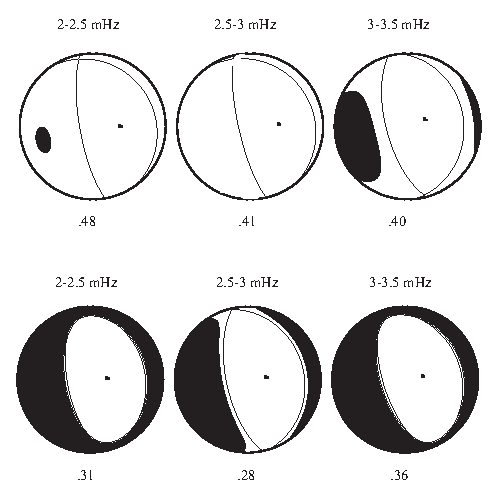
\includegraphics{../figures/chap14/fig33.eps}
\end{center}
\caption[sio]{\label{fig:14.sio}
\iffalse
Retrieved focal mechanisms for the great 1970 Colombia earthquake
in the three frequency ranges 2$-$2.5~mHz, 2.5$-$3mHz and 3$-$3.5mHz.
({\em  Top row}) Results obtained upon the spherical Earth model PREM.
({\em  Bottom row}) Results obtained upon the rotating, elliptical,
laterally heterogeneous
Earth model SKS12WM13 (Dziewonski, Liu \& Su \citeyear{liu&dziewonski96}).
A total of nineteen super-multiplets, containing between two and six
multiplets each, were incorporated in the coupled-mode analysis.
Shading denotes compressional quadrants of the focal sphere; the
P axes ({\em dots\/}) and the nodal planes of the best-fitting
double couple are also shown.
The residual variance is indicated beneath each focal mechanism.
\fi
%%%
1970~年哥伦比亚地震后,在~2$-$2.5~mHz、2.5$-$3~mHz~和~3$-$3.5~mHz~频率范围内检索的震源机制。(上图)基于球对称地球模型~PREM~的结果。(下图)基于有旋、椭球、横向不均匀地球模型~SKS12WM13(Dziewonski, Liu \& Su \citeyear{liu&dziewonski96}))的结果。总计~19~个超级多态模式(每个包含~2~至~6~个多重态)被纳入耦合模式分析中。阴影部分表示震源球的压缩象限;最优拟合双力偶的~P~轴(点)和节点面也被表示在图中。残差方差被表示在每个震源机制下。
%%%
}
\end{figure}
\iffalse
Figure~\ref{14.fig.watada1} shows that the observed
radial-component spectra $|\brh\cdot\bs(\bx,\om)|$
at stations MAJO in Matsushiro, Japan ($\Theta=81^{\circ}$)
and BKS in Berkeley, California ($\Theta=6^{\circ}$) agree
reasonably well with the corresponding spherical-Earth synthetic
spectra; however, the spectrum at station PAS in Pasadena
($\Theta<2^{\circ}$) does not.  Other nearby stations
of the broad-band TERRAscope network operated by Caltech and
the US Geological Survey exhibit a similar pattern:
the amplitudes of the long-period R2\hspace{0.3 mm}-R3,
R4\hspace{0.4 mm}-R5,$\hspace{0.3mm}\ldots$ Rayleigh wave packets are,
after propagation once or twice around the Earth, almost an order of
magnitude larger than those calculated on PREM.
\fi
%%%
图~\ref{14.fig.watada1} 表明,日本松代MAJO台站~($\Theta=81^{\circ}$)和加州伯克利BKS台站($\Theta=6^{\circ}$)的径向分量观测谱$|\brh\cdot\bs(\bx,\om)|$ 与相应的球对称地球合成谱较为吻合;然而,帕萨迪纳PAS台站($\Theta<2^{\circ}$)的频谱则完全不相符。由加州理工学院和美国地质调查局运行的宽频TERRAscope网中的其他台站呈现出类相似的样式:在绕行地球一到两次后,长周期R2\hspace{0.3 mm}-R3,
R4\hspace{0.4 mm}-R5,$\hspace{0.3mm}\ldots$瑞利波包的振幅几乎要比基于PREM的计算结果大一个数量级。
%%%
\begin{figure}[!t]
\begin{center}
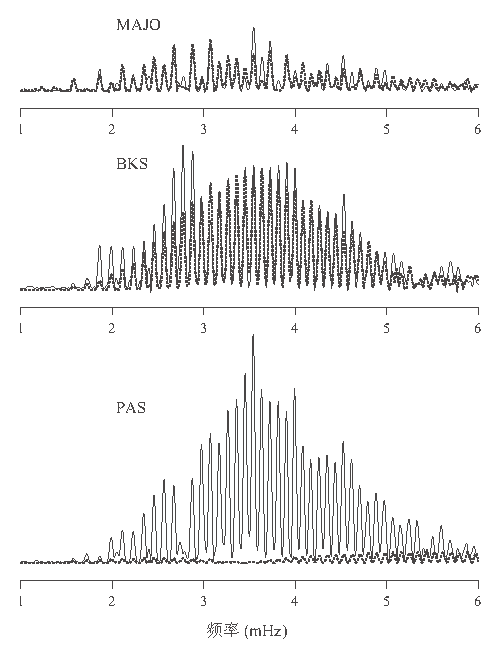
\includegraphics{../figures/chap14/fig34.eps}
\end{center}
\caption[watada1]{\label{14.fig.watada1}
\iffalse
Amplitude spectra $|\hat{\bf r}\cdot{\bf s}({\bf x},\om)|$
at MAJO ({\em top\/}), BKS ({\em middle\/})
and PAS ({\em bottom\/}) following the 1992 Landers,
California earthquake.  Both the observed spectrum
({\em solid line\/}) and the synthetic spectrum on
PREM ({\em dotted line\/}) are shown at each station.
All records have been Hann tapered, and begin at
15,000 s and end at 65,000 s after the origin time.
The vertical scale of BKS is magnified by a factor
of four relative to MAJO and PAS.  The misfit of the
BKS synthetic near 1.9 mHz and 2.8 mHz is due to the
strong Coriolis coupling of the crossover modes
${}_0{\rm S}_{11}$ and ${}_0{\rm S}_{19}$.
(Courtesy of S. Watada.)
\fi
%%%
1992~年~6~月~28~日加州兰德斯地震后,MAJO(上图)、BKS(中图)和~PAS(下图)台站的振幅谱~$|\hat{\bf r}\cdot{\bf s}({\bf x},\om)|$。实线表示每个台站处的观测谱,虚线表示~PERM~模型合成谱。对所有观测记录加汉宁窗,起始时间为第~15000~秒,结束时间为第~65000~秒。与~MAJO~和~PAS~台站相比,BKS~台站的垂直尺度增幅了~4~倍。在~1.9~和~2.8~mHz~附近,BKS~台站的合成谱失配可归结于跨支模式~${}_0{\rm S}_{11}$~和~${}_0{\rm S}_{19}$~的强科里奥利耦合。(由~S.Watada~提供)
%%%
}
\end{figure}
\iffalse
Tsuboi \& Um
(\citeyear{tsuboi&um93}) and Watada, Kanamori \& Anderson
(\citeyear{watada&al93}) have shown that this anomalous
near-field amplification is a curious consequence of the
lateral heterogeneity of the Earth---because of the associated
phase-speed perturbations, $c\rightarrow c+\delta c$, the surface
waves travel at geographically variable rates along slightly perturbed
great-circle paths, so that they no longer interfere destructively upon
arriving back in the vicinity of the source.  A complete quantitative
theory of this phenomenon needs to account for spheroidal-toroidal
Coriolis coupling as well as along-branch coupling due to the Earth's
lateral heterogeneity.  Figure~\ref{14.fig.watada2} compares the
observed Pasadena spectrum with synthetic coupled-mode spectra on
a rotating, elliptical Earth and a rotating, elliptical and laterally
heterogeneous Earth, respectively.  Five adjacent fundamental
spheroidal multiplets and five adjacent fundamental toroidal multiplets
have been used as the basis set,
to find the singlet eigenfrequencies and eigenfunctions
associated with every Coriolis-coupled target mode pair
${}_0{\rm S}_l\!-\!{}_0{\rm T}_{l\pm1}$, $0\leq l\leq 30$,
below 4 mHz.  Rotation and ellipticity alone are seen to
have a significant effect upon the near-field response;
however, they are unable to account for the observed
anomalous amplification.  The Rayleigh-wave refraction
and attendant ``non-cancellation'' caused by the
$s_{\rm max}=8$ model SH8U4L8 of the Earth's
lateral heterogeneity are, on the
other hand, able to explain almost the entire
observed effect.
More comprehensive studies by Watada,
Kanamori \& Anderson (\citeyear{watada&al93}) and Watada
(\citeyear{watada95}) indicate that the theoretical amplification
is extremely sensitive to the details of the large-scale
three-dimensional structure of the crust and upper mantle;
relatively slight adjustments to the shear-wave speed
\fi
%%%
Tsuboi \& Um~(\citeyear{tsuboi&um93})~和~Watada, Kanamori \& Anderson~(\citeyear{watada&al93})~已经表明,这种异常的近场增幅是地球横向不均匀性的一个奇怪结果--由于相关的相速微扰~$c\rightarrow c+\delta c$,面波在地理上以不同的速度沿着轻微扰动的大圆路径传播,因此当它们返回到震源附近时,就不再有相消干扰。要对这一现象进行完整的定量解释,就必须考虑由地球横向不均匀性引起的球型—环型科里奥利耦合以及同级耦合。图~\ref{14.fig.watada2}~分别比较了帕萨迪纳台站观测谱与有旋、椭球地球以及有旋、椭球和横向不均匀地球的合成耦合模式谱。利用五个相邻的基阶球型多重态和五个相邻的基阶环型多重态作为基集,求出~4~mHz~以下每个科里奥利耦合目标模式对~${}_0{\rm S}_l\!-\!{}_0{\rm T}_{l\pm1}$, $0\leq l\leq 30$~的相关单态本征频率和本征函数。自转和椭率对近场响应似乎有着独立且显著的影响;但它们无法解释观测到的异常增幅。另一方面,$s_{\rm max}=8$~阶地球横向不均匀性模型~SH8U4L8~所引起的瑞利波折射和\textcolor{red}{伴随的“不抵消”},几乎能够解释整个观测到的效应。Watada, Kanamori \& Anderson~(\citeyear{watada&al93})~和~Watada~(\citeyear{watada95})~做出了更全面的研究,表明这种理论增幅对地壳和上地幔大尺度三维结构的细节极其敏感;对剪切波速度~$\delta\hspace{-0.2 mm}\beta$~进行相对轻微的调整,就足以使合成结果与观测数据完全一致。考虑到增幅机制的性质,这种对横向不均匀性的强敏感性是可预料的。
%%%
\begin{figure}[!t]
\begin{center}
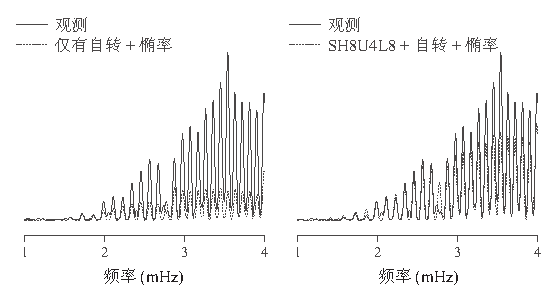
\includegraphics{../figures/chap14/fig35.eps}
\end{center}
\caption[watada2]{\label{14.fig.watada2}
\iffalse
Observed ({\em solid line\/}) and synthetic ({\em dotted line\/})
spectra at the near-field station PAS following the 1992 Landers
earthquake.  ({\em Left\/}) Effect of the Earth's rotation and
hydrostatic ellipticity.  ({\em Right\/}) Combined effect of rotation,
ellipticity and lateral heterogeneity model SH8U4L8 (Dziewonski \& Woodward
\citeyear{dziewonski&woodward92}).  Comparison with Figure~\ref{14.fig.watada1}
shows that Coriolis coupling gives rise to a slight amplification of the
response in the frequency range $2\!-\!4$ mHz.  Most of the additional effect
of model SH8U4L8 is due to the self-splitting of the fundamental spheroidal
modes; coupling along the ${}_0{\rm S}_l$ dispersion branch is fairly weak
on such a smooth Earth model.  (Courtesy of S. Watada.)
\fi
%%%
1992~年兰德斯地震后,近场台站~PAS~的观测谱(实线)和合成谱(虚线)。(左图)地球自转和流体静力学椭率效应。(右图)有旋、椭球和横向不均匀模型~SH8U4L8(Dziewonski \& Woodward~\citeyear{dziewonski&woodward92}))的联合效应。与图~\ref{14.fig.watada1}~相比,科里奥利耦合在~$2\!-\!4$~mHz~频段内的响应略有增幅。SH8U4L8~模型的大部分附加效应归结于基阶球型模式的自分裂;沿~${}_0{\rm S}_l$~频散分支的耦合效应在该平滑地球模型中相当微弱。(由~S.Watada~提供)
%%%
}
\end{figure}
\iffalse
$\delta\hspace{-0.2 mm}\beta$ are sufficient to bring
the synthetic results into full agreement with the data.
This strong sensitivity to the lateral heterogeneity is not
unexpected, given the nature of the
amplification mechanism.  In closing, we note that the
asymptotic, single great-circle approximation~(\ref{14.RomRou2})
or~(\ref{14.TOM}) is invalid in the vicinity of an
earthquake epicenter or its antipode.  A more general,
uniformly valid asymptotic approximation, which accounts
for the nearly simultaneous arrival of surface waves from
all azimuths, has been developed by Dahlen (\citeyear{dahlen80a}).
\fi
%%%
最后,我们注意到,渐近的单一大圆近似~(\ref{14.RomRou2})~或~(\ref{14.TOM})~在震中或对跖点附近是无效的。Dahlen~(\citeyear{dahlen80a})~提出了一种更常规、一致有效的渐近近似,可以解释为何来自所有方位角的面波几乎同时到达。
%%%
\index{multiplet coupling|)}%
\index{coupled mode|)}%
\index{mode!coupled|)}%
\index{Landers 1992 earthquake|)}%
